\documentclass[twoside]{book}

% Packages required by doxygen
\usepackage{calc}
\usepackage{doxygen}
\usepackage{graphicx}
\usepackage[utf8]{inputenc}
\usepackage{makeidx}
\usepackage{multicol}
\usepackage{multirow}
\usepackage{textcomp}
\usepackage[table]{xcolor}

% Font selection
\usepackage[T1]{fontenc}
\usepackage{mathptmx}
\usepackage[scaled=.90]{helvet}
\usepackage{courier}
\usepackage{amssymb}
\usepackage{sectsty}
\renewcommand{\familydefault}{\sfdefault}
\allsectionsfont{%
  \fontseries{bc}\selectfont%
  \color{darkgray}%
}
\renewcommand{\DoxyLabelFont}{%
  \fontseries{bc}\selectfont%
  \color{darkgray}%
}

% Page & text layout
\usepackage{geometry}
\geometry{%
  a4paper,%
  top=2.5cm,%
  bottom=2.5cm,%
  left=2.5cm,%
  right=2.5cm%
}
\tolerance=750
\hfuzz=15pt
\hbadness=750
\setlength{\emergencystretch}{15pt}
\setlength{\parindent}{0cm}
\setlength{\parskip}{0.2cm}
\makeatletter
\renewcommand{\paragraph}{%
  \@startsection{paragraph}{4}{0ex}{-1.0ex}{1.0ex}{%
    \normalfont\normalsize\bfseries\SS@parafont%
  }%
}
\renewcommand{\subparagraph}{%
  \@startsection{subparagraph}{5}{0ex}{-1.0ex}{1.0ex}{%
    \normalfont\normalsize\bfseries\SS@subparafont%
  }%
}
\makeatother

% Headers & footers
\usepackage{fancyhdr}
\pagestyle{fancyplain}
\fancyhead[LE]{\fancyplain{}{\bfseries\thepage}}
\fancyhead[CE]{\fancyplain{}{}}
\fancyhead[RE]{\fancyplain{}{\bfseries\leftmark}}
\fancyhead[LO]{\fancyplain{}{\bfseries\rightmark}}
\fancyhead[CO]{\fancyplain{}{}}
\fancyhead[RO]{\fancyplain{}{\bfseries\thepage}}
\fancyfoot[LE]{\fancyplain{}{}}
\fancyfoot[CE]{\fancyplain{}{}}
\fancyfoot[RE]{\fancyplain{}{\bfseries\scriptsize Generated on Tue Dec 10 2013 21\-:43\-:45 for Media\-Take by Doxygen }}
\fancyfoot[LO]{\fancyplain{}{\bfseries\scriptsize Generated on Tue Dec 10 2013 21\-:43\-:45 for Media\-Take by Doxygen }}
\fancyfoot[CO]{\fancyplain{}{}}
\fancyfoot[RO]{\fancyplain{}{}}
\renewcommand{\footrulewidth}{0.4pt}
\renewcommand{\chaptermark}[1]{%
  \markboth{#1}{}%
}
\renewcommand{\sectionmark}[1]{%
  \markright{\thesection\ #1}%
}

% Indices & bibliography
\usepackage{natbib}
\usepackage[titles]{tocloft}
\setcounter{tocdepth}{3}
\setcounter{secnumdepth}{5}
\makeindex

% Hyperlinks (required, but should be loaded last)
\usepackage{ifpdf}
\ifpdf
  \usepackage[pdftex,pagebackref=true]{hyperref}
\else
  \usepackage[ps2pdf,pagebackref=true]{hyperref}
\fi
\hypersetup{%
  colorlinks=true,%
  linkcolor=blue,%
  citecolor=blue,%
  unicode%
}

% Custom commands
\newcommand{\clearemptydoublepage}{%
  \newpage{\pagestyle{empty}\cleardoublepage}%
}


%===== C O N T E N T S =====

\begin{document}

% Titlepage & ToC
\hypersetup{pageanchor=false}
\pagenumbering{roman}
\begin{titlepage}
\vspace*{7cm}
\begin{center}%
{\Large Media\-Take \\[1ex]\large Dev id Phase 2 }\\
\vspace*{1cm}
{\large Generated by Doxygen 1.8.5}\\
\vspace*{0.5cm}
{\small Tue Dec 10 2013 21:43:45}\\
\end{center}
\end{titlepage}
\clearemptydoublepage
\tableofcontents
\clearemptydoublepage
\pagenumbering{arabic}
\hypersetup{pageanchor=true}

%--- Begin generated contents ---
\chapter{Namespace Index}
\section{Namespace List}
Here is a list of all namespaces with brief descriptions\-:\begin{DoxyCompactList}
\item\contentsline{section}{\hyperlink{namespace_ui}{Ui} }{\pageref{namespace_ui}}{}
\end{DoxyCompactList}

\chapter{Hierarchical Index}
\section{Class Hierarchy}
This inheritance list is sorted roughly, but not completely, alphabetically\-:\begin{DoxyCompactList}
\item Q\-Dialog\begin{DoxyCompactList}
\item \contentsline{section}{Select\-File\-Dialog}{\pageref{class_select_file_dialog}}{}
\end{DoxyCompactList}
\item Q\-Main\-Window\begin{DoxyCompactList}
\item \contentsline{section}{Main\-Window}{\pageref{class_main_window}}{}
\item \contentsline{section}{Video\-Sink}{\pageref{class_video_sink}}{}
\end{DoxyCompactList}
\item Q\-Thread\begin{DoxyCompactList}
\item \contentsline{section}{Database\-Operations}{\pageref{class_database_operations}}{}
\begin{DoxyCompactList}
\item \contentsline{section}{Database\-Operations\-Audio}{\pageref{class_database_operations_audio}}{}
\begin{DoxyCompactList}
\item \contentsline{section}{File\-Finder\-Audio}{\pageref{class_file_finder_audio}}{}
\begin{DoxyCompactList}
\item \contentsline{section}{Library\-Manager\-Audio}{\pageref{class_library_manager_audio}}{}
\end{DoxyCompactList}
\end{DoxyCompactList}
\item \contentsline{section}{Database\-Operations\-Video}{\pageref{class_database_operations_video}}{}
\begin{DoxyCompactList}
\item \contentsline{section}{File\-Finder\-Video}{\pageref{class_file_finder_video}}{}
\begin{DoxyCompactList}
\item \contentsline{section}{Library\-Manager\-Video}{\pageref{class_library_manager_video}}{}
\end{DoxyCompactList}
\end{DoxyCompactList}
\end{DoxyCompactList}
\end{DoxyCompactList}
\item Video\-Widget\begin{DoxyCompactList}
\item \contentsline{section}{Qt\-G\-Streamer\-Driver}{\pageref{class_qt_g_streamer_driver}}{}
\end{DoxyCompactList}
\end{DoxyCompactList}

\chapter{Class Index}
\section{Class List}
Here are the classes, structs, unions and interfaces with brief descriptions\-:\begin{DoxyCompactList}
\item\contentsline{section}{\hyperlink{class_database_operations}{Database\-Operations} }{\pageref{class_database_operations}}{}
\item\contentsline{section}{\hyperlink{class_database_operations_audio}{Database\-Operations\-Audio} }{\pageref{class_database_operations_audio}}{}
\item\contentsline{section}{\hyperlink{class_database_operations_video}{Database\-Operations\-Video} }{\pageref{class_database_operations_video}}{}
\item\contentsline{section}{\hyperlink{class_file_finder_audio}{File\-Finder\-Audio} }{\pageref{class_file_finder_audio}}{}
\item\contentsline{section}{\hyperlink{class_file_finder_video}{File\-Finder\-Video} }{\pageref{class_file_finder_video}}{}
\item\contentsline{section}{\hyperlink{class_library_manager_audio}{Library\-Manager\-Audio} }{\pageref{class_library_manager_audio}}{}
\item\contentsline{section}{\hyperlink{class_library_manager_video}{Library\-Manager\-Video} }{\pageref{class_library_manager_video}}{}
\item\contentsline{section}{\hyperlink{class_main_window}{Main\-Window} }{\pageref{class_main_window}}{}
\item\contentsline{section}{\hyperlink{class_qt_g_streamer_driver}{Qt\-G\-Streamer\-Driver} }{\pageref{class_qt_g_streamer_driver}}{}
\item\contentsline{section}{\hyperlink{class_select_file_dialog}{Select\-File\-Dialog} }{\pageref{class_select_file_dialog}}{}
\item\contentsline{section}{\hyperlink{class_video_sink}{Video\-Sink} }{\pageref{class_video_sink}}{}
\end{DoxyCompactList}

\chapter{File Index}
\section{File List}
Here is a list of all files with brief descriptions\-:\begin{DoxyCompactList}
\item\contentsline{section}{C\-:/\-Users/\-X/\-Documents/\-Qt/\-Media\-Take/\hyperlink{databaseoperations_8cpp}{databaseoperations.\-cpp} }{\pageref{databaseoperations_8cpp}}{}
\item\contentsline{section}{C\-:/\-Users/\-X/\-Documents/\-Qt/\-Media\-Take/\hyperlink{databaseoperations_8h}{databaseoperations.\-h} }{\pageref{databaseoperations_8h}}{}
\item\contentsline{section}{C\-:/\-Users/\-X/\-Documents/\-Qt/\-Media\-Take/\hyperlink{databaseoperationsaudio_8cpp}{databaseoperationsaudio.\-cpp} }{\pageref{databaseoperationsaudio_8cpp}}{}
\item\contentsline{section}{C\-:/\-Users/\-X/\-Documents/\-Qt/\-Media\-Take/\hyperlink{databaseoperationsaudio_8h}{databaseoperationsaudio.\-h} }{\pageref{databaseoperationsaudio_8h}}{}
\item\contentsline{section}{C\-:/\-Users/\-X/\-Documents/\-Qt/\-Media\-Take/\hyperlink{databaseoperationsvideo_8cpp}{databaseoperationsvideo.\-cpp} }{\pageref{databaseoperationsvideo_8cpp}}{}
\item\contentsline{section}{C\-:/\-Users/\-X/\-Documents/\-Qt/\-Media\-Take/\hyperlink{databaseoperationsvideo_8h}{databaseoperationsvideo.\-h} }{\pageref{databaseoperationsvideo_8h}}{}
\item\contentsline{section}{C\-:/\-Users/\-X/\-Documents/\-Qt/\-Media\-Take/\hyperlink{filefinderaudio_8cpp}{filefinderaudio.\-cpp} }{\pageref{filefinderaudio_8cpp}}{}
\item\contentsline{section}{C\-:/\-Users/\-X/\-Documents/\-Qt/\-Media\-Take/\hyperlink{filefinderaudio_8h}{filefinderaudio.\-h} }{\pageref{filefinderaudio_8h}}{}
\item\contentsline{section}{C\-:/\-Users/\-X/\-Documents/\-Qt/\-Media\-Take/\hyperlink{filefindervideo_8cpp}{filefindervideo.\-cpp} }{\pageref{filefindervideo_8cpp}}{}
\item\contentsline{section}{C\-:/\-Users/\-X/\-Documents/\-Qt/\-Media\-Take/\hyperlink{filefindervideo_8h}{filefindervideo.\-h} }{\pageref{filefindervideo_8h}}{}
\item\contentsline{section}{C\-:/\-Users/\-X/\-Documents/\-Qt/\-Media\-Take/\hyperlink{librarymanageraudio_8cpp}{librarymanageraudio.\-cpp} }{\pageref{librarymanageraudio_8cpp}}{}
\item\contentsline{section}{C\-:/\-Users/\-X/\-Documents/\-Qt/\-Media\-Take/\hyperlink{librarymanageraudio_8h}{librarymanageraudio.\-h} }{\pageref{librarymanageraudio_8h}}{}
\item\contentsline{section}{C\-:/\-Users/\-X/\-Documents/\-Qt/\-Media\-Take/\hyperlink{librarymanagervideo_8cpp}{librarymanagervideo.\-cpp} }{\pageref{librarymanagervideo_8cpp}}{}
\item\contentsline{section}{C\-:/\-Users/\-X/\-Documents/\-Qt/\-Media\-Take/\hyperlink{librarymanagervideo_8h}{librarymanagervideo.\-h} }{\pageref{librarymanagervideo_8h}}{}
\item\contentsline{section}{C\-:/\-Users/\-X/\-Documents/\-Qt/\-Media\-Take/\hyperlink{main_8cpp}{main.\-cpp} }{\pageref{main_8cpp}}{}
\item\contentsline{section}{C\-:/\-Users/\-X/\-Documents/\-Qt/\-Media\-Take/\hyperlink{mainwindow_8cpp}{mainwindow.\-cpp} }{\pageref{mainwindow_8cpp}}{}
\item\contentsline{section}{C\-:/\-Users/\-X/\-Documents/\-Qt/\-Media\-Take/\hyperlink{mainwindow_8h}{mainwindow.\-h} }{\pageref{mainwindow_8h}}{}
\item\contentsline{section}{C\-:/\-Users/\-X/\-Documents/\-Qt/\-Media\-Take/\hyperlink{qtgstreamerdriver_8cpp}{qtgstreamerdriver.\-cpp} }{\pageref{qtgstreamerdriver_8cpp}}{}
\item\contentsline{section}{C\-:/\-Users/\-X/\-Documents/\-Qt/\-Media\-Take/\hyperlink{qtgstreamerdriver_8h}{qtgstreamerdriver.\-h} }{\pageref{qtgstreamerdriver_8h}}{}
\item\contentsline{section}{C\-:/\-Users/\-X/\-Documents/\-Qt/\-Media\-Take/\hyperlink{selectfiledialog_8cpp}{selectfiledialog.\-cpp} }{\pageref{selectfiledialog_8cpp}}{}
\item\contentsline{section}{C\-:/\-Users/\-X/\-Documents/\-Qt/\-Media\-Take/\hyperlink{selectfiledialog_8h}{selectfiledialog.\-h} }{\pageref{selectfiledialog_8h}}{}
\item\contentsline{section}{C\-:/\-Users/\-X/\-Documents/\-Qt/\-Media\-Take/\hyperlink{videosink_8cpp}{videosink.\-cpp} }{\pageref{videosink_8cpp}}{}
\item\contentsline{section}{C\-:/\-Users/\-X/\-Documents/\-Qt/\-Media\-Take/\hyperlink{videosink_8h}{videosink.\-h} }{\pageref{videosink_8h}}{}
\end{DoxyCompactList}

\chapter{Namespace Documentation}
\hypertarget{namespace_ui}{\section{Ui Namespace Reference}
\label{namespace_ui}\index{Ui@{Ui}}
}

\chapter{Class Documentation}
\hypertarget{class_database_operations}{\section{Database\-Operations Class Reference}
\label{class_database_operations}\index{Database\-Operations@{Database\-Operations}}
}


{\ttfamily \#include $<$databaseoperations.\-h$>$}



Inheritance diagram for Database\-Operations\-:
\nopagebreak
\begin{figure}[H]
\begin{center}
\leavevmode
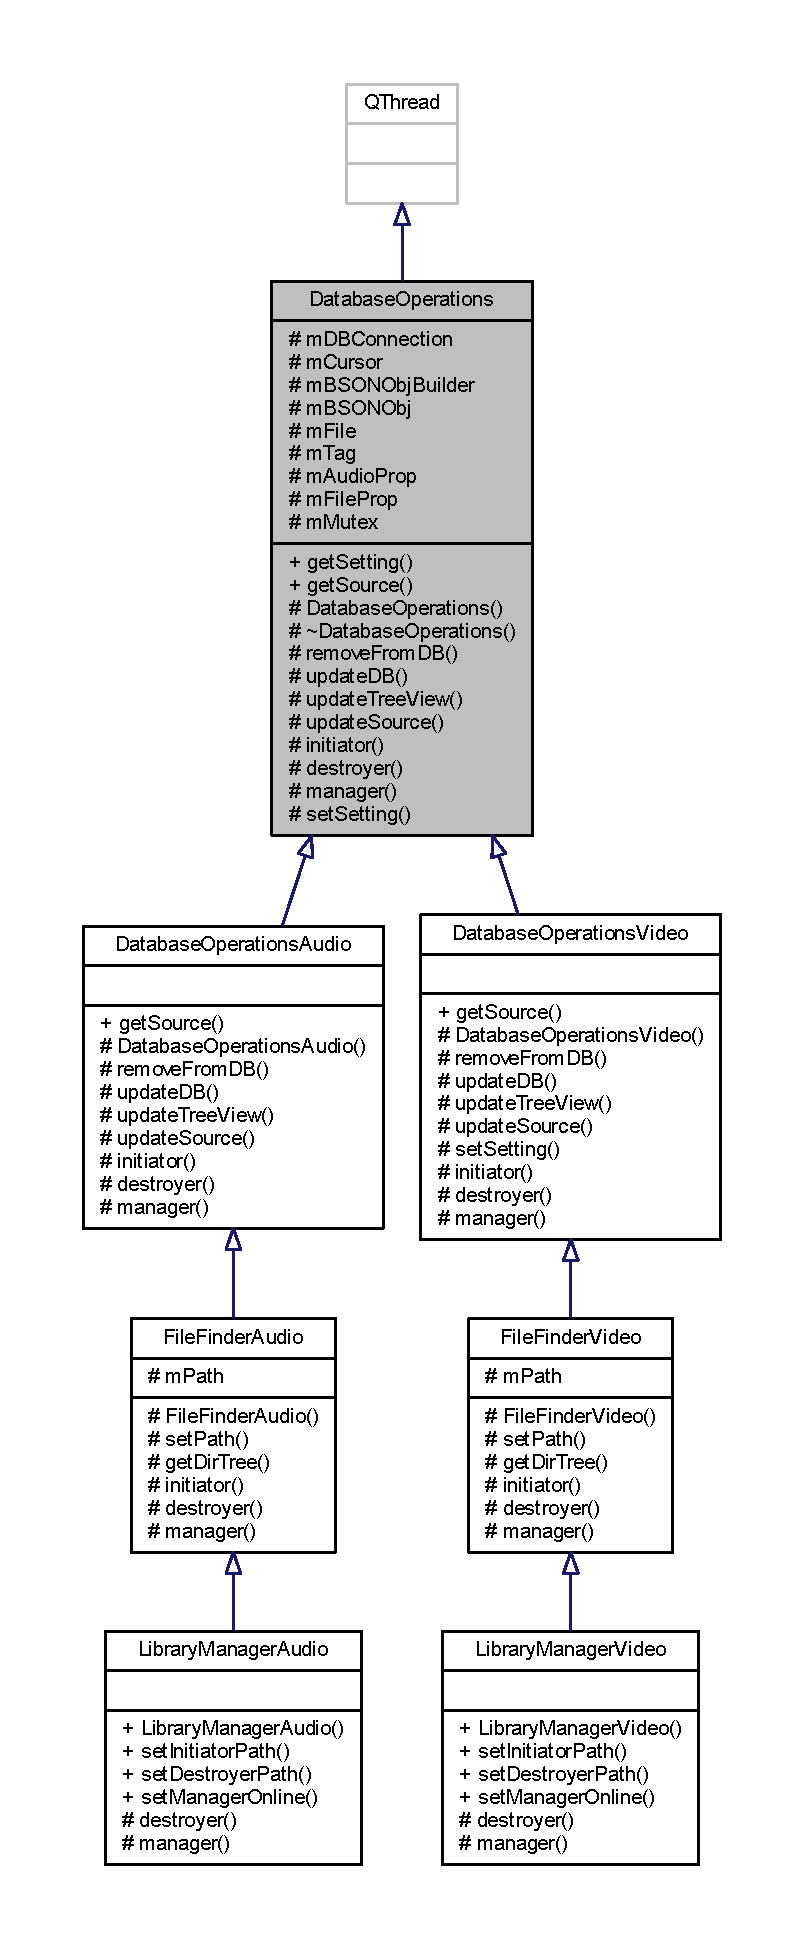
\includegraphics[height=550pt]{class_database_operations__inherit__graph}
\end{center}
\end{figure}


Collaboration diagram for Database\-Operations\-:
\nopagebreak
\begin{figure}[H]
\begin{center}
\leavevmode
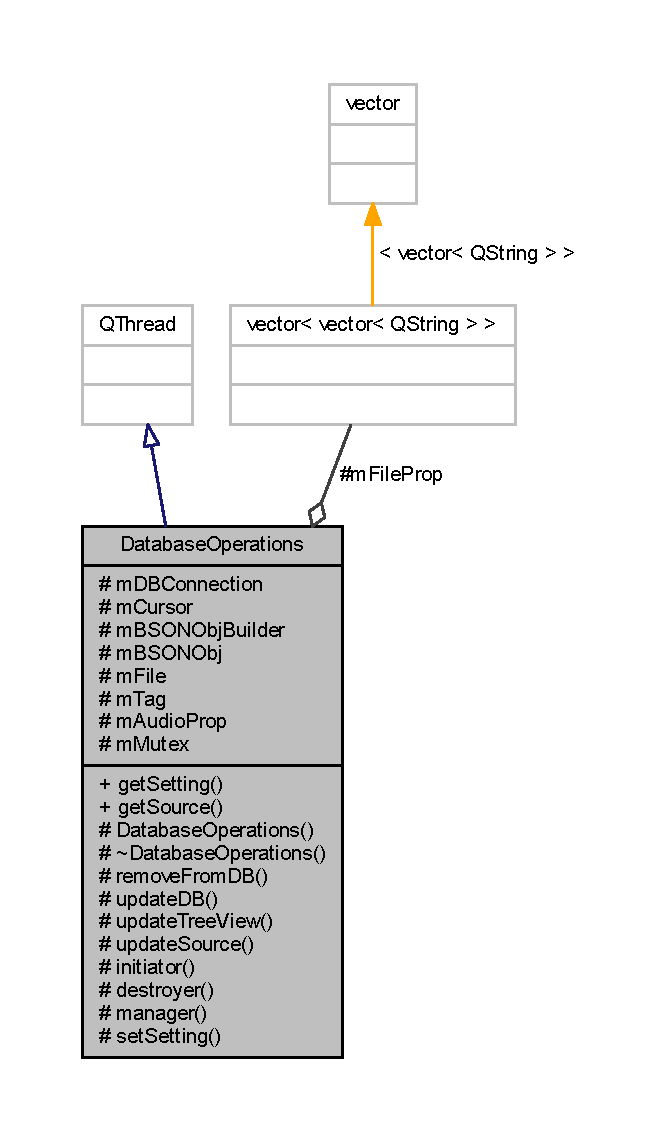
\includegraphics[width=317pt]{class_database_operations__coll__graph}
\end{center}
\end{figure}
\subsection*{Signals}
\begin{DoxyCompactItemize}
\item 
virtual void \hyperlink{class_database_operations_a31fab20336d2bb54e41983b4db5a87cc}{update\-Tree\-Widget\-Library\-Display} (vector$<$ vector$<$ Q\-String $>$ $>$)=0
\item 
virtual void \hyperlink{class_database_operations_ad920f83b72e1184bc844cc5002b2c13a}{update\-Path} (Q\-String)=0
\end{DoxyCompactItemize}
\subsection*{Public Member Functions}
\begin{DoxyCompactItemize}
\item 
void \hyperlink{class_database_operations_a7fb19eb6129268920bc655321703fa0d}{get\-Setting} ()
\item 
virtual void \hyperlink{class_database_operations_a8cf9e78c2927df5cc0a886992d394fdd}{get\-Source} ()=0
\end{DoxyCompactItemize}
\subsection*{Protected Member Functions}
\begin{DoxyCompactItemize}
\item 
\hyperlink{class_database_operations_a843d8a6cc96a346a1ab4943362a9ba0c}{Database\-Operations} (Q\-Object $\ast$parent=0)
\item 
virtual \hyperlink{class_database_operations_a512890dc178ab17b5d54592fbba0eabd}{$\sim$\-Database\-Operations} ()
\item 
virtual void \hyperlink{class_database_operations_abab54bc65a349871c58d6027d871786e}{remove\-From\-D\-B} (Q\-String)=0
\item 
virtual void \hyperlink{class_database_operations_afe6635240b49bdeb4a1cee1b948da5fd}{update\-D\-B} (Q\-String, Q\-File\-Info, Q\-File\-Info\-List)=0
\item 
virtual void \hyperlink{class_database_operations_a77a4a371cfb8fdc2fc0cbf0f954693cd}{update\-Tree\-View} ()=0
\item 
virtual void \hyperlink{class_database_operations_a78b632e484e7d469f02366dbd9e1cd91}{update\-Source} (Q\-String)=0
\item 
virtual void \hyperlink{class_database_operations_af399d5ee2e6c559cf98c3ca6559f96e5}{initiator} ()=0
\item 
virtual void \hyperlink{class_database_operations_a435467e14c7ebdf3ecc6359e57c4d013}{destroyer} ()=0
\item 
virtual void \hyperlink{class_database_operations_aeacfe0c761bf321b7a0c45763a16b4cf}{manager} ()=0
\item 
void \hyperlink{class_database_operations_a2d74da811fa9cb8f0239bfea76ccb9d4}{set\-Setting} ()
\end{DoxyCompactItemize}
\subsection*{Protected Attributes}
\begin{DoxyCompactItemize}
\item 
mongo\-::\-D\-B\-Client\-Connection \hyperlink{class_database_operations_a407ee7c24b774c93bd7d915566c84663}{m\-D\-B\-Connection}
\item 
mongo\-::auto\-\_\-ptr\\*
$<$ mongo\-::\-D\-B\-Client\-Cursor $>$ \hyperlink{class_database_operations_a0768987f8c116148aae4175cfc0df6bd}{m\-Cursor}
\item 
mongo\-::\-B\-S\-O\-N\-Obj\-Builder $\ast$ \hyperlink{class_database_operations_ae6604cf6874bd9700ee3158c35945687}{m\-B\-S\-O\-N\-Obj\-Builder}
\item 
mongo\-::\-B\-S\-O\-N\-Obj \hyperlink{class_database_operations_a40636866ce3a84961ed1c241e6ee0885}{m\-B\-S\-O\-N\-Obj}
\item 
Tag\-Lib\-::\-File\-Ref $\ast$ \hyperlink{class_database_operations_af61f0200ac06733bbd9276faf9fa4488}{m\-File}
\item 
Tag\-Lib\-::\-Tag $\ast$ \hyperlink{class_database_operations_a4ee540c45bc895889be44c652693d0e5}{m\-Tag}
\item 
Tag\-Lib\-::\-Audio\-Properties $\ast$ \hyperlink{class_database_operations_a5cf34cf709fe0574fe5101b4f1818a23}{m\-Audio\-Prop}
\item 
vector$<$ vector$<$ Q\-String $>$ $>$ \hyperlink{class_database_operations_a27137305ac34557b97fdffd8e17a9be2}{m\-File\-Prop}
\item 
Q\-Mutex \hyperlink{class_database_operations_a527401ca7671c2856b6368cad0c1c3a7}{m\-Mutex}
\end{DoxyCompactItemize}


\subsection{Detailed Description}


Definition at line 27 of file databaseoperations.\-h.



\subsection{Constructor \& Destructor Documentation}
\hypertarget{class_database_operations_a843d8a6cc96a346a1ab4943362a9ba0c}{\index{Database\-Operations@{Database\-Operations}!Database\-Operations@{Database\-Operations}}
\index{Database\-Operations@{Database\-Operations}!DatabaseOperations@{Database\-Operations}}
\subsubsection[{Database\-Operations}]{\setlength{\rightskip}{0pt plus 5cm}Database\-Operations\-::\-Database\-Operations (
\begin{DoxyParamCaption}
\item[{Q\-Object $\ast$}]{parent = {\ttfamily 0}}
\end{DoxyParamCaption}
)\hspace{0.3cm}{\ttfamily [explicit]}, {\ttfamily [protected]}}}\label{class_database_operations_a843d8a6cc96a346a1ab4943362a9ba0c}


Definition at line 4 of file databaseoperations.\-cpp.

\hypertarget{class_database_operations_a512890dc178ab17b5d54592fbba0eabd}{\index{Database\-Operations@{Database\-Operations}!$\sim$\-Database\-Operations@{$\sim$\-Database\-Operations}}
\index{$\sim$\-Database\-Operations@{$\sim$\-Database\-Operations}!DatabaseOperations@{Database\-Operations}}
\subsubsection[{$\sim$\-Database\-Operations}]{\setlength{\rightskip}{0pt plus 5cm}Database\-Operations\-::$\sim$\-Database\-Operations (
\begin{DoxyParamCaption}
{}
\end{DoxyParamCaption}
)\hspace{0.3cm}{\ttfamily [protected]}, {\ttfamily [virtual]}}}\label{class_database_operations_a512890dc178ab17b5d54592fbba0eabd}


Definition at line 16 of file databaseoperations.\-cpp.



\subsection{Member Function Documentation}
\hypertarget{class_database_operations_a435467e14c7ebdf3ecc6359e57c4d013}{\index{Database\-Operations@{Database\-Operations}!destroyer@{destroyer}}
\index{destroyer@{destroyer}!DatabaseOperations@{Database\-Operations}}
\subsubsection[{destroyer}]{\setlength{\rightskip}{0pt plus 5cm}virtual void Database\-Operations\-::destroyer (
\begin{DoxyParamCaption}
{}
\end{DoxyParamCaption}
)\hspace{0.3cm}{\ttfamily [protected]}, {\ttfamily [pure virtual]}}}\label{class_database_operations_a435467e14c7ebdf3ecc6359e57c4d013}


Implemented in \hyperlink{class_file_finder_audio_aeab95a78219b1fb187da1cae16a6b9c8}{File\-Finder\-Audio}, \hyperlink{class_file_finder_video_a37f0b885d2e98d3ac8b6f845c874c63d}{File\-Finder\-Video}, \hyperlink{class_library_manager_audio_af69df97c95e9e0fae6b08d071b9ab93d}{Library\-Manager\-Audio}, \hyperlink{class_database_operations_video_ab2b75036caeaa73cedc14e591d628580}{Database\-Operations\-Video}, \hyperlink{class_library_manager_video_abdecc35f2d907679a08f32ef8749b9bc}{Library\-Manager\-Video}, and \hyperlink{class_database_operations_audio_ab4879167601725f2faf7a69d73aa2309}{Database\-Operations\-Audio}.

\hypertarget{class_database_operations_a7fb19eb6129268920bc655321703fa0d}{\index{Database\-Operations@{Database\-Operations}!get\-Setting@{get\-Setting}}
\index{get\-Setting@{get\-Setting}!DatabaseOperations@{Database\-Operations}}
\subsubsection[{get\-Setting}]{\setlength{\rightskip}{0pt plus 5cm}void Database\-Operations\-::get\-Setting (
\begin{DoxyParamCaption}
{}
\end{DoxyParamCaption}
)}}\label{class_database_operations_a7fb19eb6129268920bc655321703fa0d}
\hypertarget{class_database_operations_a8cf9e78c2927df5cc0a886992d394fdd}{\index{Database\-Operations@{Database\-Operations}!get\-Source@{get\-Source}}
\index{get\-Source@{get\-Source}!DatabaseOperations@{Database\-Operations}}
\subsubsection[{get\-Source}]{\setlength{\rightskip}{0pt plus 5cm}virtual void Database\-Operations\-::get\-Source (
\begin{DoxyParamCaption}
{}
\end{DoxyParamCaption}
)\hspace{0.3cm}{\ttfamily [pure virtual]}}}\label{class_database_operations_a8cf9e78c2927df5cc0a886992d394fdd}


Implemented in \hyperlink{class_database_operations_video_a16849f71aa872f601c6651b43e786dab}{Database\-Operations\-Video}, and \hyperlink{class_database_operations_audio_afd2ea7e19882b60d4b991875eb886347}{Database\-Operations\-Audio}.

\hypertarget{class_database_operations_af399d5ee2e6c559cf98c3ca6559f96e5}{\index{Database\-Operations@{Database\-Operations}!initiator@{initiator}}
\index{initiator@{initiator}!DatabaseOperations@{Database\-Operations}}
\subsubsection[{initiator}]{\setlength{\rightskip}{0pt plus 5cm}virtual void Database\-Operations\-::initiator (
\begin{DoxyParamCaption}
{}
\end{DoxyParamCaption}
)\hspace{0.3cm}{\ttfamily [protected]}, {\ttfamily [pure virtual]}}}\label{class_database_operations_af399d5ee2e6c559cf98c3ca6559f96e5}


Implemented in \hyperlink{class_file_finder_audio_af8153dd34e8691aab1445413b3a86d12}{File\-Finder\-Audio}, \hyperlink{class_file_finder_video_ad792218f1dafd62852f7d25bc3b80a50}{File\-Finder\-Video}, \hyperlink{class_database_operations_video_ab541cb7de9ff375af08e5e32ca1b217f}{Database\-Operations\-Video}, and \hyperlink{class_database_operations_audio_a80507c96dabef6ca3a06a0d3f83fb657}{Database\-Operations\-Audio}.

\hypertarget{class_database_operations_aeacfe0c761bf321b7a0c45763a16b4cf}{\index{Database\-Operations@{Database\-Operations}!manager@{manager}}
\index{manager@{manager}!DatabaseOperations@{Database\-Operations}}
\subsubsection[{manager}]{\setlength{\rightskip}{0pt plus 5cm}virtual void Database\-Operations\-::manager (
\begin{DoxyParamCaption}
{}
\end{DoxyParamCaption}
)\hspace{0.3cm}{\ttfamily [protected]}, {\ttfamily [pure virtual]}}}\label{class_database_operations_aeacfe0c761bf321b7a0c45763a16b4cf}


Implemented in \hyperlink{class_file_finder_audio_ab11c9010b5031e4e251e2fe592ea6321}{File\-Finder\-Audio}, \hyperlink{class_file_finder_video_aafe5126b440c0c5564a32a54fee0781c}{File\-Finder\-Video}, \hyperlink{class_library_manager_audio_ad2176013457295b02726edb2e6a547c4}{Library\-Manager\-Audio}, \hyperlink{class_database_operations_video_a54a804b782a0653e58a53c25040d3f85}{Database\-Operations\-Video}, \hyperlink{class_library_manager_video_a414263df76f62ab14a3372ba983cd348}{Library\-Manager\-Video}, and \hyperlink{class_database_operations_audio_a7db082335a6a48ce277383f5382c15c2}{Database\-Operations\-Audio}.

\hypertarget{class_database_operations_abab54bc65a349871c58d6027d871786e}{\index{Database\-Operations@{Database\-Operations}!remove\-From\-D\-B@{remove\-From\-D\-B}}
\index{remove\-From\-D\-B@{remove\-From\-D\-B}!DatabaseOperations@{Database\-Operations}}
\subsubsection[{remove\-From\-D\-B}]{\setlength{\rightskip}{0pt plus 5cm}virtual void Database\-Operations\-::remove\-From\-D\-B (
\begin{DoxyParamCaption}
\item[{Q\-String}]{}
\end{DoxyParamCaption}
)\hspace{0.3cm}{\ttfamily [protected]}, {\ttfamily [pure virtual]}}}\label{class_database_operations_abab54bc65a349871c58d6027d871786e}


Implemented in \hyperlink{class_database_operations_video_a3187c0433cbc90c9cbcbd091bfc76e9d}{Database\-Operations\-Video}, and \hyperlink{class_database_operations_audio_a0e819c77ddae10bdaac2666e0be372a3}{Database\-Operations\-Audio}.

\hypertarget{class_database_operations_a2d74da811fa9cb8f0239bfea76ccb9d4}{\index{Database\-Operations@{Database\-Operations}!set\-Setting@{set\-Setting}}
\index{set\-Setting@{set\-Setting}!DatabaseOperations@{Database\-Operations}}
\subsubsection[{set\-Setting}]{\setlength{\rightskip}{0pt plus 5cm}void Database\-Operations\-::set\-Setting (
\begin{DoxyParamCaption}
{}
\end{DoxyParamCaption}
)\hspace{0.3cm}{\ttfamily [protected]}}}\label{class_database_operations_a2d74da811fa9cb8f0239bfea76ccb9d4}
\hypertarget{class_database_operations_afe6635240b49bdeb4a1cee1b948da5fd}{\index{Database\-Operations@{Database\-Operations}!update\-D\-B@{update\-D\-B}}
\index{update\-D\-B@{update\-D\-B}!DatabaseOperations@{Database\-Operations}}
\subsubsection[{update\-D\-B}]{\setlength{\rightskip}{0pt plus 5cm}virtual void Database\-Operations\-::update\-D\-B (
\begin{DoxyParamCaption}
\item[{Q\-String}]{, }
\item[{Q\-File\-Info}]{, }
\item[{Q\-File\-Info\-List}]{}
\end{DoxyParamCaption}
)\hspace{0.3cm}{\ttfamily [protected]}, {\ttfamily [pure virtual]}}}\label{class_database_operations_afe6635240b49bdeb4a1cee1b948da5fd}


Implemented in \hyperlink{class_database_operations_video_a2e0c44a699ccc0b6248549bffe8078f9}{Database\-Operations\-Video}, and \hyperlink{class_database_operations_audio_ad0a8ec0e0472aed58a9927e00cd5a7fd}{Database\-Operations\-Audio}.

\hypertarget{class_database_operations_ad920f83b72e1184bc844cc5002b2c13a}{\index{Database\-Operations@{Database\-Operations}!update\-Path@{update\-Path}}
\index{update\-Path@{update\-Path}!DatabaseOperations@{Database\-Operations}}
\subsubsection[{update\-Path}]{\setlength{\rightskip}{0pt plus 5cm}virtual void Database\-Operations\-::update\-Path (
\begin{DoxyParamCaption}
\item[{Q\-String}]{}
\end{DoxyParamCaption}
)\hspace{0.3cm}{\ttfamily [pure virtual]}, {\ttfamily [signal]}}}\label{class_database_operations_ad920f83b72e1184bc844cc5002b2c13a}
\hypertarget{class_database_operations_a78b632e484e7d469f02366dbd9e1cd91}{\index{Database\-Operations@{Database\-Operations}!update\-Source@{update\-Source}}
\index{update\-Source@{update\-Source}!DatabaseOperations@{Database\-Operations}}
\subsubsection[{update\-Source}]{\setlength{\rightskip}{0pt plus 5cm}virtual void Database\-Operations\-::update\-Source (
\begin{DoxyParamCaption}
\item[{Q\-String}]{}
\end{DoxyParamCaption}
)\hspace{0.3cm}{\ttfamily [protected]}, {\ttfamily [pure virtual]}}}\label{class_database_operations_a78b632e484e7d469f02366dbd9e1cd91}


Implemented in \hyperlink{class_database_operations_video_ac5c4d66e50e9342eede8f63d91057756}{Database\-Operations\-Video}, and \hyperlink{class_database_operations_audio_a1dc402c2c29b384e1015dea77fcf3662}{Database\-Operations\-Audio}.

\hypertarget{class_database_operations_a77a4a371cfb8fdc2fc0cbf0f954693cd}{\index{Database\-Operations@{Database\-Operations}!update\-Tree\-View@{update\-Tree\-View}}
\index{update\-Tree\-View@{update\-Tree\-View}!DatabaseOperations@{Database\-Operations}}
\subsubsection[{update\-Tree\-View}]{\setlength{\rightskip}{0pt plus 5cm}virtual void Database\-Operations\-::update\-Tree\-View (
\begin{DoxyParamCaption}
{}
\end{DoxyParamCaption}
)\hspace{0.3cm}{\ttfamily [protected]}, {\ttfamily [pure virtual]}}}\label{class_database_operations_a77a4a371cfb8fdc2fc0cbf0f954693cd}


Implemented in \hyperlink{class_database_operations_video_a958ad3432e96e3c51664bb687b244d06}{Database\-Operations\-Video}, and \hyperlink{class_database_operations_audio_a42d73126a8b2822f84a040aa604f9925}{Database\-Operations\-Audio}.

\hypertarget{class_database_operations_a31fab20336d2bb54e41983b4db5a87cc}{\index{Database\-Operations@{Database\-Operations}!update\-Tree\-Widget\-Library\-Display@{update\-Tree\-Widget\-Library\-Display}}
\index{update\-Tree\-Widget\-Library\-Display@{update\-Tree\-Widget\-Library\-Display}!DatabaseOperations@{Database\-Operations}}
\subsubsection[{update\-Tree\-Widget\-Library\-Display}]{\setlength{\rightskip}{0pt plus 5cm}virtual void Database\-Operations\-::update\-Tree\-Widget\-Library\-Display (
\begin{DoxyParamCaption}
\item[{vector$<$ vector$<$ Q\-String $>$ $>$}]{}
\end{DoxyParamCaption}
)\hspace{0.3cm}{\ttfamily [pure virtual]}, {\ttfamily [signal]}}}\label{class_database_operations_a31fab20336d2bb54e41983b4db5a87cc}


\subsection{Member Data Documentation}
\hypertarget{class_database_operations_a5cf34cf709fe0574fe5101b4f1818a23}{\index{Database\-Operations@{Database\-Operations}!m\-Audio\-Prop@{m\-Audio\-Prop}}
\index{m\-Audio\-Prop@{m\-Audio\-Prop}!DatabaseOperations@{Database\-Operations}}
\subsubsection[{m\-Audio\-Prop}]{\setlength{\rightskip}{0pt plus 5cm}Tag\-Lib\-::\-Audio\-Properties$\ast$ Database\-Operations\-::m\-Audio\-Prop\hspace{0.3cm}{\ttfamily [protected]}}}\label{class_database_operations_a5cf34cf709fe0574fe5101b4f1818a23}


Definition at line 46 of file databaseoperations.\-h.

\hypertarget{class_database_operations_a40636866ce3a84961ed1c241e6ee0885}{\index{Database\-Operations@{Database\-Operations}!m\-B\-S\-O\-N\-Obj@{m\-B\-S\-O\-N\-Obj}}
\index{m\-B\-S\-O\-N\-Obj@{m\-B\-S\-O\-N\-Obj}!DatabaseOperations@{Database\-Operations}}
\subsubsection[{m\-B\-S\-O\-N\-Obj}]{\setlength{\rightskip}{0pt plus 5cm}mongo\-::\-B\-S\-O\-N\-Obj Database\-Operations\-::m\-B\-S\-O\-N\-Obj\hspace{0.3cm}{\ttfamily [protected]}}}\label{class_database_operations_a40636866ce3a84961ed1c241e6ee0885}


Definition at line 42 of file databaseoperations.\-h.

\hypertarget{class_database_operations_ae6604cf6874bd9700ee3158c35945687}{\index{Database\-Operations@{Database\-Operations}!m\-B\-S\-O\-N\-Obj\-Builder@{m\-B\-S\-O\-N\-Obj\-Builder}}
\index{m\-B\-S\-O\-N\-Obj\-Builder@{m\-B\-S\-O\-N\-Obj\-Builder}!DatabaseOperations@{Database\-Operations}}
\subsubsection[{m\-B\-S\-O\-N\-Obj\-Builder}]{\setlength{\rightskip}{0pt plus 5cm}mongo\-::\-B\-S\-O\-N\-Obj\-Builder$\ast$ Database\-Operations\-::m\-B\-S\-O\-N\-Obj\-Builder\hspace{0.3cm}{\ttfamily [protected]}}}\label{class_database_operations_ae6604cf6874bd9700ee3158c35945687}


Definition at line 41 of file databaseoperations.\-h.

\hypertarget{class_database_operations_a0768987f8c116148aae4175cfc0df6bd}{\index{Database\-Operations@{Database\-Operations}!m\-Cursor@{m\-Cursor}}
\index{m\-Cursor@{m\-Cursor}!DatabaseOperations@{Database\-Operations}}
\subsubsection[{m\-Cursor}]{\setlength{\rightskip}{0pt plus 5cm}mongo\-::auto\-\_\-ptr$<$mongo\-::\-D\-B\-Client\-Cursor$>$ Database\-Operations\-::m\-Cursor\hspace{0.3cm}{\ttfamily [protected]}}}\label{class_database_operations_a0768987f8c116148aae4175cfc0df6bd}


Definition at line 38 of file databaseoperations.\-h.

\hypertarget{class_database_operations_a407ee7c24b774c93bd7d915566c84663}{\index{Database\-Operations@{Database\-Operations}!m\-D\-B\-Connection@{m\-D\-B\-Connection}}
\index{m\-D\-B\-Connection@{m\-D\-B\-Connection}!DatabaseOperations@{Database\-Operations}}
\subsubsection[{m\-D\-B\-Connection}]{\setlength{\rightskip}{0pt plus 5cm}mongo\-::\-D\-B\-Client\-Connection Database\-Operations\-::m\-D\-B\-Connection\hspace{0.3cm}{\ttfamily [protected]}}}\label{class_database_operations_a407ee7c24b774c93bd7d915566c84663}


Definition at line 37 of file databaseoperations.\-h.

\hypertarget{class_database_operations_af61f0200ac06733bbd9276faf9fa4488}{\index{Database\-Operations@{Database\-Operations}!m\-File@{m\-File}}
\index{m\-File@{m\-File}!DatabaseOperations@{Database\-Operations}}
\subsubsection[{m\-File}]{\setlength{\rightskip}{0pt plus 5cm}Tag\-Lib\-::\-File\-Ref$\ast$ Database\-Operations\-::m\-File\hspace{0.3cm}{\ttfamily [protected]}}}\label{class_database_operations_af61f0200ac06733bbd9276faf9fa4488}


Definition at line 44 of file databaseoperations.\-h.

\hypertarget{class_database_operations_a27137305ac34557b97fdffd8e17a9be2}{\index{Database\-Operations@{Database\-Operations}!m\-File\-Prop@{m\-File\-Prop}}
\index{m\-File\-Prop@{m\-File\-Prop}!DatabaseOperations@{Database\-Operations}}
\subsubsection[{m\-File\-Prop}]{\setlength{\rightskip}{0pt plus 5cm}vector$<$ vector $<$ Q\-String $>$ $>$ Database\-Operations\-::m\-File\-Prop\hspace{0.3cm}{\ttfamily [protected]}}}\label{class_database_operations_a27137305ac34557b97fdffd8e17a9be2}


Definition at line 49 of file databaseoperations.\-h.

\hypertarget{class_database_operations_a527401ca7671c2856b6368cad0c1c3a7}{\index{Database\-Operations@{Database\-Operations}!m\-Mutex@{m\-Mutex}}
\index{m\-Mutex@{m\-Mutex}!DatabaseOperations@{Database\-Operations}}
\subsubsection[{m\-Mutex}]{\setlength{\rightskip}{0pt plus 5cm}Q\-Mutex Database\-Operations\-::m\-Mutex\hspace{0.3cm}{\ttfamily [protected]}}}\label{class_database_operations_a527401ca7671c2856b6368cad0c1c3a7}


Definition at line 51 of file databaseoperations.\-h.

\hypertarget{class_database_operations_a4ee540c45bc895889be44c652693d0e5}{\index{Database\-Operations@{Database\-Operations}!m\-Tag@{m\-Tag}}
\index{m\-Tag@{m\-Tag}!DatabaseOperations@{Database\-Operations}}
\subsubsection[{m\-Tag}]{\setlength{\rightskip}{0pt plus 5cm}Tag\-Lib\-::\-Tag$\ast$ Database\-Operations\-::m\-Tag\hspace{0.3cm}{\ttfamily [protected]}}}\label{class_database_operations_a4ee540c45bc895889be44c652693d0e5}


Definition at line 45 of file databaseoperations.\-h.



The documentation for this class was generated from the following files\-:\begin{DoxyCompactItemize}
\item 
C\-:/\-Users/\-X/\-Documents/\-Qt/\-Media\-Take/\hyperlink{databaseoperations_8h}{databaseoperations.\-h}\item 
C\-:/\-Users/\-X/\-Documents/\-Qt/\-Media\-Take/\hyperlink{databaseoperations_8cpp}{databaseoperations.\-cpp}\end{DoxyCompactItemize}

\hypertarget{class_database_operations_audio}{\section{Database\-Operations\-Audio Class Reference}
\label{class_database_operations_audio}\index{Database\-Operations\-Audio@{Database\-Operations\-Audio}}
}


{\ttfamily \#include $<$databaseoperationsaudio.\-h$>$}



Inheritance diagram for Database\-Operations\-Audio\-:
\nopagebreak
\begin{figure}[H]
\begin{center}
\leavevmode
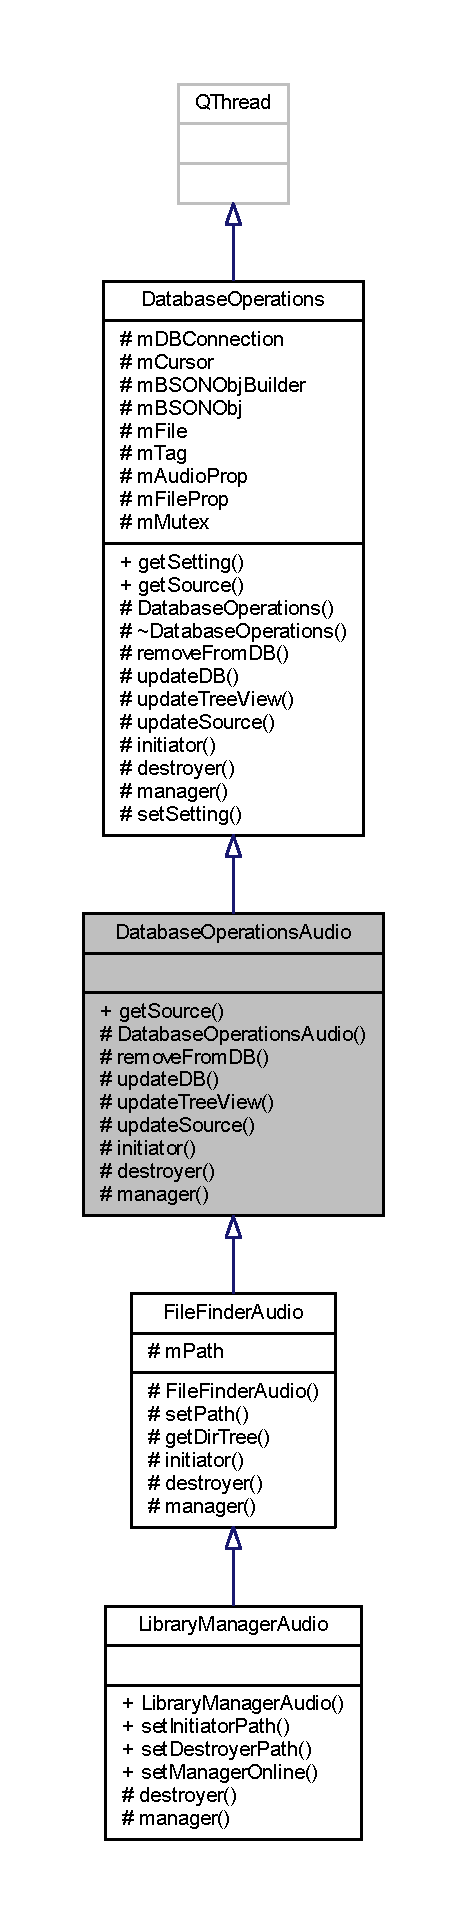
\includegraphics[height=550pt]{class_database_operations_audio__inherit__graph}
\end{center}
\end{figure}


Collaboration diagram for Database\-Operations\-Audio\-:
\nopagebreak
\begin{figure}[H]
\begin{center}
\leavevmode
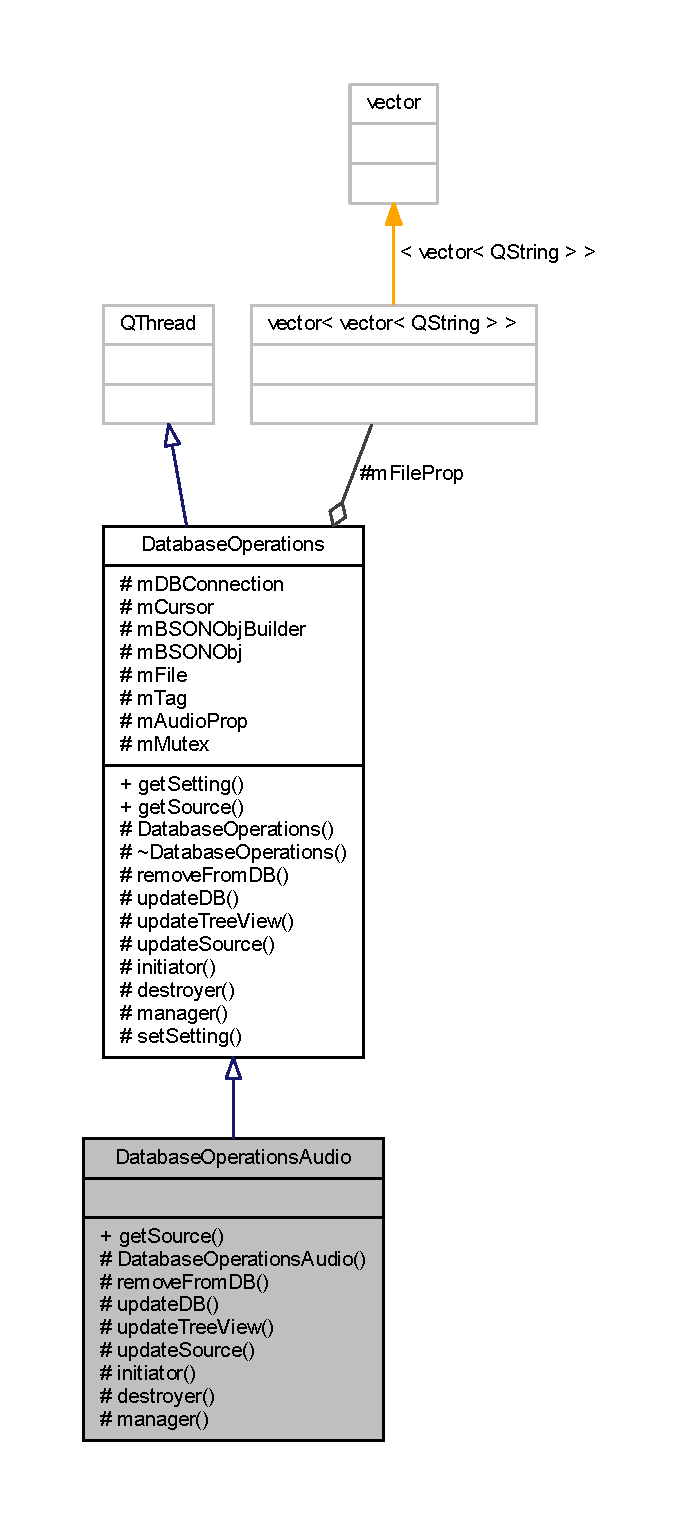
\includegraphics[height=550pt]{class_database_operations_audio__coll__graph}
\end{center}
\end{figure}
\subsection*{Signals}
\begin{DoxyCompactItemize}
\item 
void \hyperlink{class_database_operations_audio_a663fb07afd5d0c4c0b0de23fd2c19ad1}{update\-Tree\-Widget\-Library\-Display} (vector$<$ vector$<$ Q\-String $>$ $>$)
\item 
void \hyperlink{class_database_operations_audio_ae28ef899c95c7b5d660d1898f97a0052}{update\-Path} (Q\-String)
\end{DoxyCompactItemize}
\subsection*{Public Member Functions}
\begin{DoxyCompactItemize}
\item 
void \hyperlink{class_database_operations_audio_afd2ea7e19882b60d4b991875eb886347}{get\-Source} ()
\end{DoxyCompactItemize}
\subsection*{Protected Member Functions}
\begin{DoxyCompactItemize}
\item 
\hyperlink{class_database_operations_audio_a078a5fbf2535364118cea60e8fb739c4}{Database\-Operations\-Audio} (Q\-Object $\ast$parent=0)
\item 
void \hyperlink{class_database_operations_audio_a0e819c77ddae10bdaac2666e0be372a3}{remove\-From\-D\-B} (Q\-String)
\item 
void \hyperlink{class_database_operations_audio_ad0a8ec0e0472aed58a9927e00cd5a7fd}{update\-D\-B} (Q\-String, Q\-File\-Info, Q\-File\-Info\-List)
\item 
void \hyperlink{class_database_operations_audio_a42d73126a8b2822f84a040aa604f9925}{update\-Tree\-View} ()
\item 
void \hyperlink{class_database_operations_audio_a1dc402c2c29b384e1015dea77fcf3662}{update\-Source} (Q\-String)
\item 
virtual void \hyperlink{class_database_operations_audio_a80507c96dabef6ca3a06a0d3f83fb657}{initiator} ()=0
\item 
virtual void \hyperlink{class_database_operations_audio_ab4879167601725f2faf7a69d73aa2309}{destroyer} ()=0
\item 
virtual void \hyperlink{class_database_operations_audio_a7db082335a6a48ce277383f5382c15c2}{manager} ()=0
\end{DoxyCompactItemize}
\subsection*{Additional Inherited Members}


\subsection{Detailed Description}


Definition at line 5 of file databaseoperationsaudio.\-h.



\subsection{Constructor \& Destructor Documentation}
\hypertarget{class_database_operations_audio_a078a5fbf2535364118cea60e8fb739c4}{\index{Database\-Operations\-Audio@{Database\-Operations\-Audio}!Database\-Operations\-Audio@{Database\-Operations\-Audio}}
\index{Database\-Operations\-Audio@{Database\-Operations\-Audio}!DatabaseOperationsAudio@{Database\-Operations\-Audio}}
\subsubsection[{Database\-Operations\-Audio}]{\setlength{\rightskip}{0pt plus 5cm}Database\-Operations\-Audio\-::\-Database\-Operations\-Audio (
\begin{DoxyParamCaption}
\item[{Q\-Object $\ast$}]{parent = {\ttfamily 0}}
\end{DoxyParamCaption}
)\hspace{0.3cm}{\ttfamily [explicit]}, {\ttfamily [protected]}}}\label{class_database_operations_audio_a078a5fbf2535364118cea60e8fb739c4}


Definition at line 3 of file databaseoperationsaudio.\-cpp.



\subsection{Member Function Documentation}
\hypertarget{class_database_operations_audio_ab4879167601725f2faf7a69d73aa2309}{\index{Database\-Operations\-Audio@{Database\-Operations\-Audio}!destroyer@{destroyer}}
\index{destroyer@{destroyer}!DatabaseOperationsAudio@{Database\-Operations\-Audio}}
\subsubsection[{destroyer}]{\setlength{\rightskip}{0pt plus 5cm}virtual void Database\-Operations\-Audio\-::destroyer (
\begin{DoxyParamCaption}
{}
\end{DoxyParamCaption}
)\hspace{0.3cm}{\ttfamily [protected]}, {\ttfamily [pure virtual]}}}\label{class_database_operations_audio_ab4879167601725f2faf7a69d73aa2309}


Implements \hyperlink{class_database_operations_a435467e14c7ebdf3ecc6359e57c4d013}{Database\-Operations}.



Implemented in \hyperlink{class_file_finder_audio_aeab95a78219b1fb187da1cae16a6b9c8}{File\-Finder\-Audio}, and \hyperlink{class_library_manager_audio_af69df97c95e9e0fae6b08d071b9ab93d}{Library\-Manager\-Audio}.

\hypertarget{class_database_operations_audio_afd2ea7e19882b60d4b991875eb886347}{\index{Database\-Operations\-Audio@{Database\-Operations\-Audio}!get\-Source@{get\-Source}}
\index{get\-Source@{get\-Source}!DatabaseOperationsAudio@{Database\-Operations\-Audio}}
\subsubsection[{get\-Source}]{\setlength{\rightskip}{0pt plus 5cm}void Database\-Operations\-Audio\-::get\-Source (
\begin{DoxyParamCaption}
{}
\end{DoxyParamCaption}
)\hspace{0.3cm}{\ttfamily [virtual]}}}\label{class_database_operations_audio_afd2ea7e19882b60d4b991875eb886347}


Implements \hyperlink{class_database_operations_a8cf9e78c2927df5cc0a886992d394fdd}{Database\-Operations}.



Definition at line 8 of file databaseoperationsaudio.\-cpp.



Here is the caller graph for this function\-:
\nopagebreak
\begin{figure}[H]
\begin{center}
\leavevmode
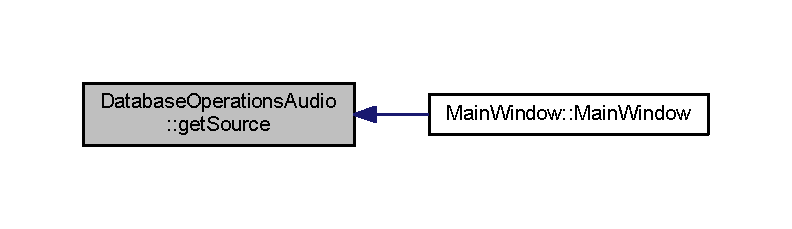
\includegraphics[width=350pt]{class_database_operations_audio_afd2ea7e19882b60d4b991875eb886347_icgraph}
\end{center}
\end{figure}


\hypertarget{class_database_operations_audio_a80507c96dabef6ca3a06a0d3f83fb657}{\index{Database\-Operations\-Audio@{Database\-Operations\-Audio}!initiator@{initiator}}
\index{initiator@{initiator}!DatabaseOperationsAudio@{Database\-Operations\-Audio}}
\subsubsection[{initiator}]{\setlength{\rightskip}{0pt plus 5cm}virtual void Database\-Operations\-Audio\-::initiator (
\begin{DoxyParamCaption}
{}
\end{DoxyParamCaption}
)\hspace{0.3cm}{\ttfamily [protected]}, {\ttfamily [pure virtual]}}}\label{class_database_operations_audio_a80507c96dabef6ca3a06a0d3f83fb657}


Implements \hyperlink{class_database_operations_af399d5ee2e6c559cf98c3ca6559f96e5}{Database\-Operations}.



Implemented in \hyperlink{class_file_finder_audio_af8153dd34e8691aab1445413b3a86d12}{File\-Finder\-Audio}.

\hypertarget{class_database_operations_audio_a7db082335a6a48ce277383f5382c15c2}{\index{Database\-Operations\-Audio@{Database\-Operations\-Audio}!manager@{manager}}
\index{manager@{manager}!DatabaseOperationsAudio@{Database\-Operations\-Audio}}
\subsubsection[{manager}]{\setlength{\rightskip}{0pt plus 5cm}virtual void Database\-Operations\-Audio\-::manager (
\begin{DoxyParamCaption}
{}
\end{DoxyParamCaption}
)\hspace{0.3cm}{\ttfamily [protected]}, {\ttfamily [pure virtual]}}}\label{class_database_operations_audio_a7db082335a6a48ce277383f5382c15c2}


Implements \hyperlink{class_database_operations_aeacfe0c761bf321b7a0c45763a16b4cf}{Database\-Operations}.



Implemented in \hyperlink{class_file_finder_audio_ab11c9010b5031e4e251e2fe592ea6321}{File\-Finder\-Audio}, and \hyperlink{class_library_manager_audio_ad2176013457295b02726edb2e6a547c4}{Library\-Manager\-Audio}.

\hypertarget{class_database_operations_audio_a0e819c77ddae10bdaac2666e0be372a3}{\index{Database\-Operations\-Audio@{Database\-Operations\-Audio}!remove\-From\-D\-B@{remove\-From\-D\-B}}
\index{remove\-From\-D\-B@{remove\-From\-D\-B}!DatabaseOperationsAudio@{Database\-Operations\-Audio}}
\subsubsection[{remove\-From\-D\-B}]{\setlength{\rightskip}{0pt plus 5cm}void Database\-Operations\-Audio\-::remove\-From\-D\-B (
\begin{DoxyParamCaption}
\item[{Q\-String}]{v\-Path}
\end{DoxyParamCaption}
)\hspace{0.3cm}{\ttfamily [protected]}, {\ttfamily [virtual]}}}\label{class_database_operations_audio_a0e819c77ddae10bdaac2666e0be372a3}


Implements \hyperlink{class_database_operations_abab54bc65a349871c58d6027d871786e}{Database\-Operations}.



Definition at line 202 of file databaseoperationsaudio.\-cpp.



Here is the caller graph for this function\-:
\nopagebreak
\begin{figure}[H]
\begin{center}
\leavevmode
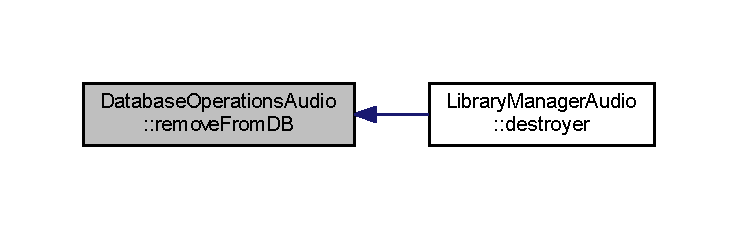
\includegraphics[width=350pt]{class_database_operations_audio_a0e819c77ddae10bdaac2666e0be372a3_icgraph}
\end{center}
\end{figure}


\hypertarget{class_database_operations_audio_ad0a8ec0e0472aed58a9927e00cd5a7fd}{\index{Database\-Operations\-Audio@{Database\-Operations\-Audio}!update\-D\-B@{update\-D\-B}}
\index{update\-D\-B@{update\-D\-B}!DatabaseOperationsAudio@{Database\-Operations\-Audio}}
\subsubsection[{update\-D\-B}]{\setlength{\rightskip}{0pt plus 5cm}void Database\-Operations\-Audio\-::update\-D\-B (
\begin{DoxyParamCaption}
\item[{Q\-String}]{v\-Source, }
\item[{Q\-File\-Info}]{v\-Parent, }
\item[{Q\-File\-Info\-List}]{v\-Children}
\end{DoxyParamCaption}
)\hspace{0.3cm}{\ttfamily [protected]}, {\ttfamily [virtual]}}}\label{class_database_operations_audio_ad0a8ec0e0472aed58a9927e00cd5a7fd}


Implements \hyperlink{class_database_operations_afe6635240b49bdeb4a1cee1b948da5fd}{Database\-Operations}.



Definition at line 21 of file databaseoperationsaudio.\-cpp.



Here is the caller graph for this function\-:
\nopagebreak
\begin{figure}[H]
\begin{center}
\leavevmode
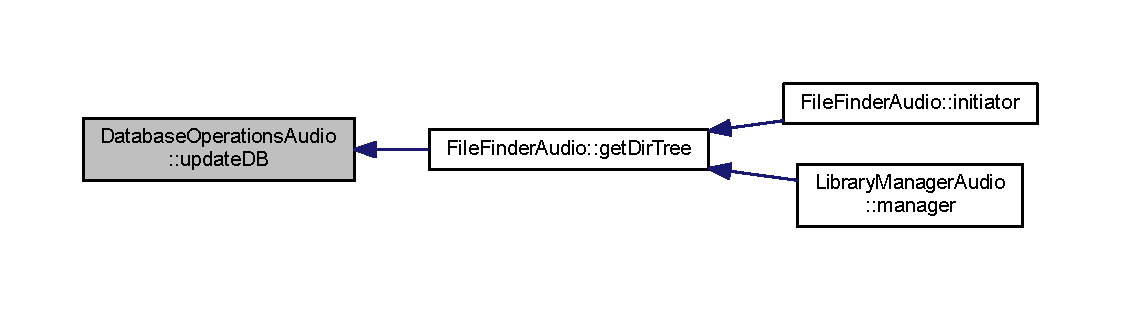
\includegraphics[width=350pt]{class_database_operations_audio_ad0a8ec0e0472aed58a9927e00cd5a7fd_icgraph}
\end{center}
\end{figure}


\hypertarget{class_database_operations_audio_ae28ef899c95c7b5d660d1898f97a0052}{\index{Database\-Operations\-Audio@{Database\-Operations\-Audio}!update\-Path@{update\-Path}}
\index{update\-Path@{update\-Path}!DatabaseOperationsAudio@{Database\-Operations\-Audio}}
\subsubsection[{update\-Path}]{\setlength{\rightskip}{0pt plus 5cm}void Database\-Operations\-Audio\-::update\-Path (
\begin{DoxyParamCaption}
\item[{Q\-String}]{}
\end{DoxyParamCaption}
)\hspace{0.3cm}{\ttfamily [signal]}}}\label{class_database_operations_audio_ae28ef899c95c7b5d660d1898f97a0052}


Here is the caller graph for this function\-:
\nopagebreak
\begin{figure}[H]
\begin{center}
\leavevmode
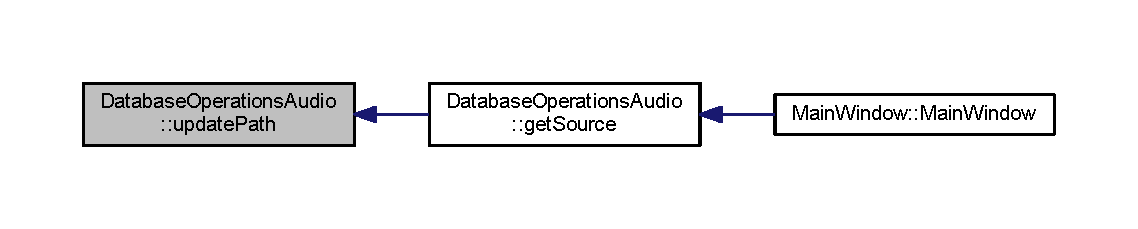
\includegraphics[width=350pt]{class_database_operations_audio_ae28ef899c95c7b5d660d1898f97a0052_icgraph}
\end{center}
\end{figure}


\hypertarget{class_database_operations_audio_a1dc402c2c29b384e1015dea77fcf3662}{\index{Database\-Operations\-Audio@{Database\-Operations\-Audio}!update\-Source@{update\-Source}}
\index{update\-Source@{update\-Source}!DatabaseOperationsAudio@{Database\-Operations\-Audio}}
\subsubsection[{update\-Source}]{\setlength{\rightskip}{0pt plus 5cm}void Database\-Operations\-Audio\-::update\-Source (
\begin{DoxyParamCaption}
\item[{Q\-String}]{v\-Path}
\end{DoxyParamCaption}
)\hspace{0.3cm}{\ttfamily [protected]}, {\ttfamily [virtual]}}}\label{class_database_operations_audio_a1dc402c2c29b384e1015dea77fcf3662}


Implements \hyperlink{class_database_operations_a78b632e484e7d469f02366dbd9e1cd91}{Database\-Operations}.



Definition at line 181 of file databaseoperationsaudio.\-cpp.



Here is the caller graph for this function\-:
\nopagebreak
\begin{figure}[H]
\begin{center}
\leavevmode
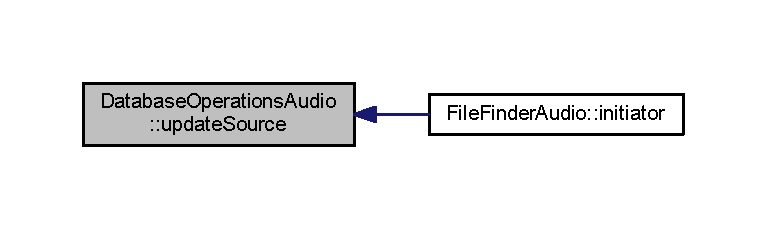
\includegraphics[width=350pt]{class_database_operations_audio_a1dc402c2c29b384e1015dea77fcf3662_icgraph}
\end{center}
\end{figure}


\hypertarget{class_database_operations_audio_a42d73126a8b2822f84a040aa604f9925}{\index{Database\-Operations\-Audio@{Database\-Operations\-Audio}!update\-Tree\-View@{update\-Tree\-View}}
\index{update\-Tree\-View@{update\-Tree\-View}!DatabaseOperationsAudio@{Database\-Operations\-Audio}}
\subsubsection[{update\-Tree\-View}]{\setlength{\rightskip}{0pt plus 5cm}void Database\-Operations\-Audio\-::update\-Tree\-View (
\begin{DoxyParamCaption}
{}
\end{DoxyParamCaption}
)\hspace{0.3cm}{\ttfamily [protected]}, {\ttfamily [virtual]}}}\label{class_database_operations_audio_a42d73126a8b2822f84a040aa604f9925}


Implements \hyperlink{class_database_operations_a77a4a371cfb8fdc2fc0cbf0f954693cd}{Database\-Operations}.



Definition at line 146 of file databaseoperationsaudio.\-cpp.



Here is the caller graph for this function\-:
\nopagebreak
\begin{figure}[H]
\begin{center}
\leavevmode
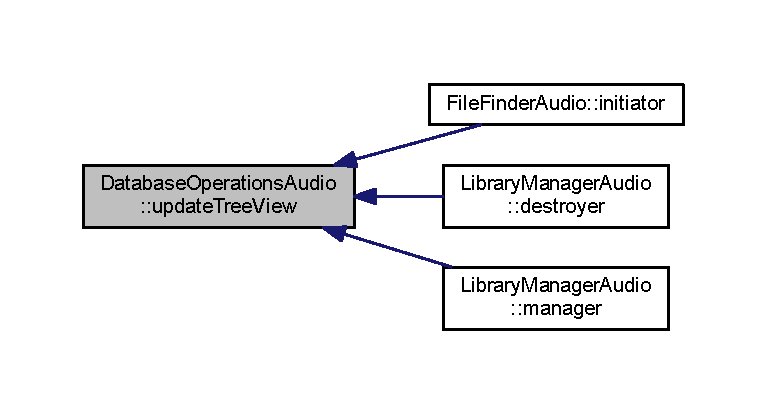
\includegraphics[width=350pt]{class_database_operations_audio_a42d73126a8b2822f84a040aa604f9925_icgraph}
\end{center}
\end{figure}


\hypertarget{class_database_operations_audio_a663fb07afd5d0c4c0b0de23fd2c19ad1}{\index{Database\-Operations\-Audio@{Database\-Operations\-Audio}!update\-Tree\-Widget\-Library\-Display@{update\-Tree\-Widget\-Library\-Display}}
\index{update\-Tree\-Widget\-Library\-Display@{update\-Tree\-Widget\-Library\-Display}!DatabaseOperationsAudio@{Database\-Operations\-Audio}}
\subsubsection[{update\-Tree\-Widget\-Library\-Display}]{\setlength{\rightskip}{0pt plus 5cm}void Database\-Operations\-Audio\-::update\-Tree\-Widget\-Library\-Display (
\begin{DoxyParamCaption}
\item[{vector$<$ vector$<$ Q\-String $>$ $>$}]{}
\end{DoxyParamCaption}
)\hspace{0.3cm}{\ttfamily [signal]}}}\label{class_database_operations_audio_a663fb07afd5d0c4c0b0de23fd2c19ad1}


Here is the caller graph for this function\-:
\nopagebreak
\begin{figure}[H]
\begin{center}
\leavevmode
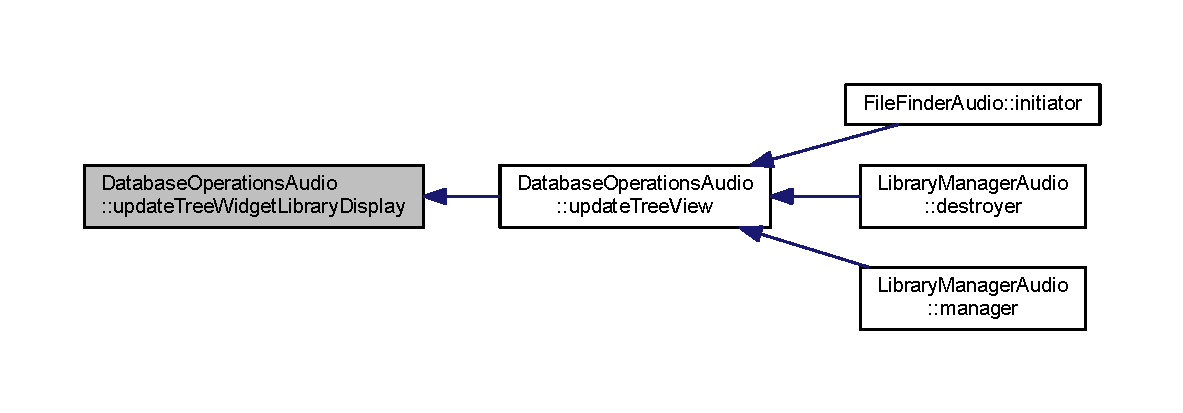
\includegraphics[width=350pt]{class_database_operations_audio_a663fb07afd5d0c4c0b0de23fd2c19ad1_icgraph}
\end{center}
\end{figure}




The documentation for this class was generated from the following files\-:\begin{DoxyCompactItemize}
\item 
C\-:/\-Users/\-X/\-Documents/\-Qt/\-Media\-Take/\hyperlink{databaseoperationsaudio_8h}{databaseoperationsaudio.\-h}\item 
C\-:/\-Users/\-X/\-Documents/\-Qt/\-Media\-Take/\hyperlink{databaseoperationsaudio_8cpp}{databaseoperationsaudio.\-cpp}\end{DoxyCompactItemize}

\hypertarget{class_database_operations_video}{\section{Database\-Operations\-Video Class Reference}
\label{class_database_operations_video}\index{Database\-Operations\-Video@{Database\-Operations\-Video}}
}


{\ttfamily \#include $<$databaseoperationsvideo.\-h$>$}



Inheritance diagram for Database\-Operations\-Video\-:
\nopagebreak
\begin{figure}[H]
\begin{center}
\leavevmode
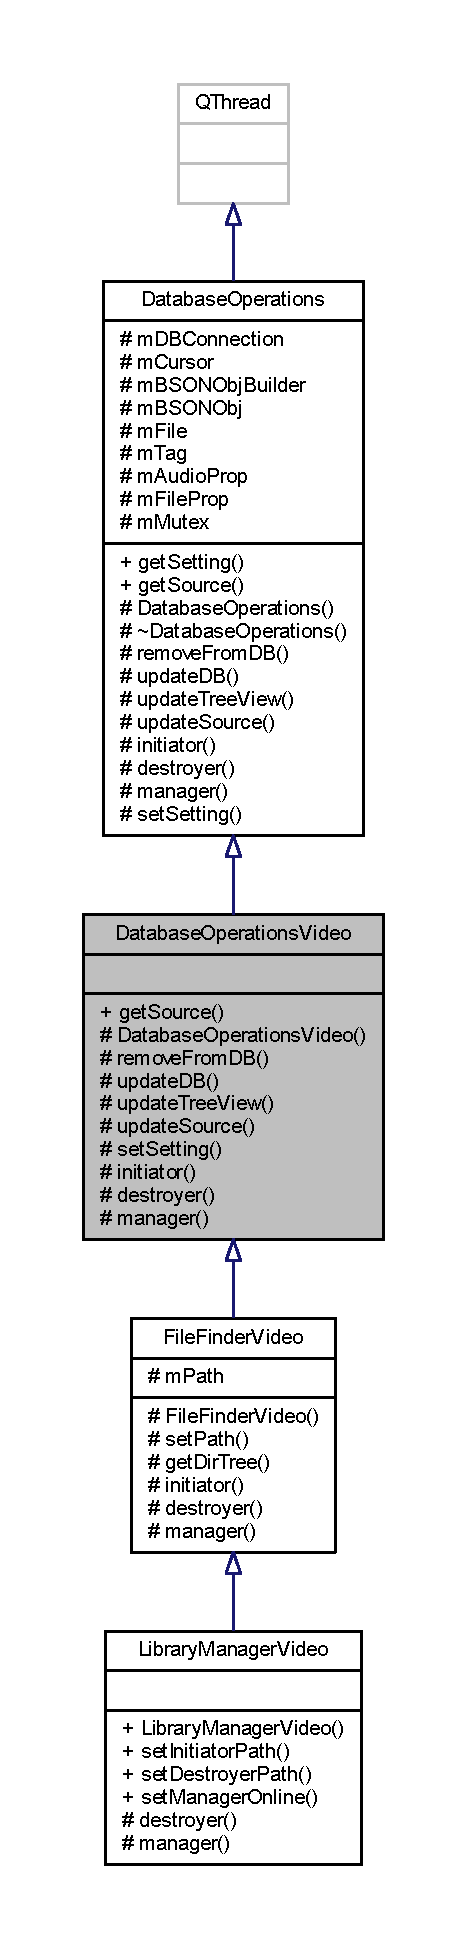
\includegraphics[height=550pt]{class_database_operations_video__inherit__graph}
\end{center}
\end{figure}


Collaboration diagram for Database\-Operations\-Video\-:
\nopagebreak
\begin{figure}[H]
\begin{center}
\leavevmode
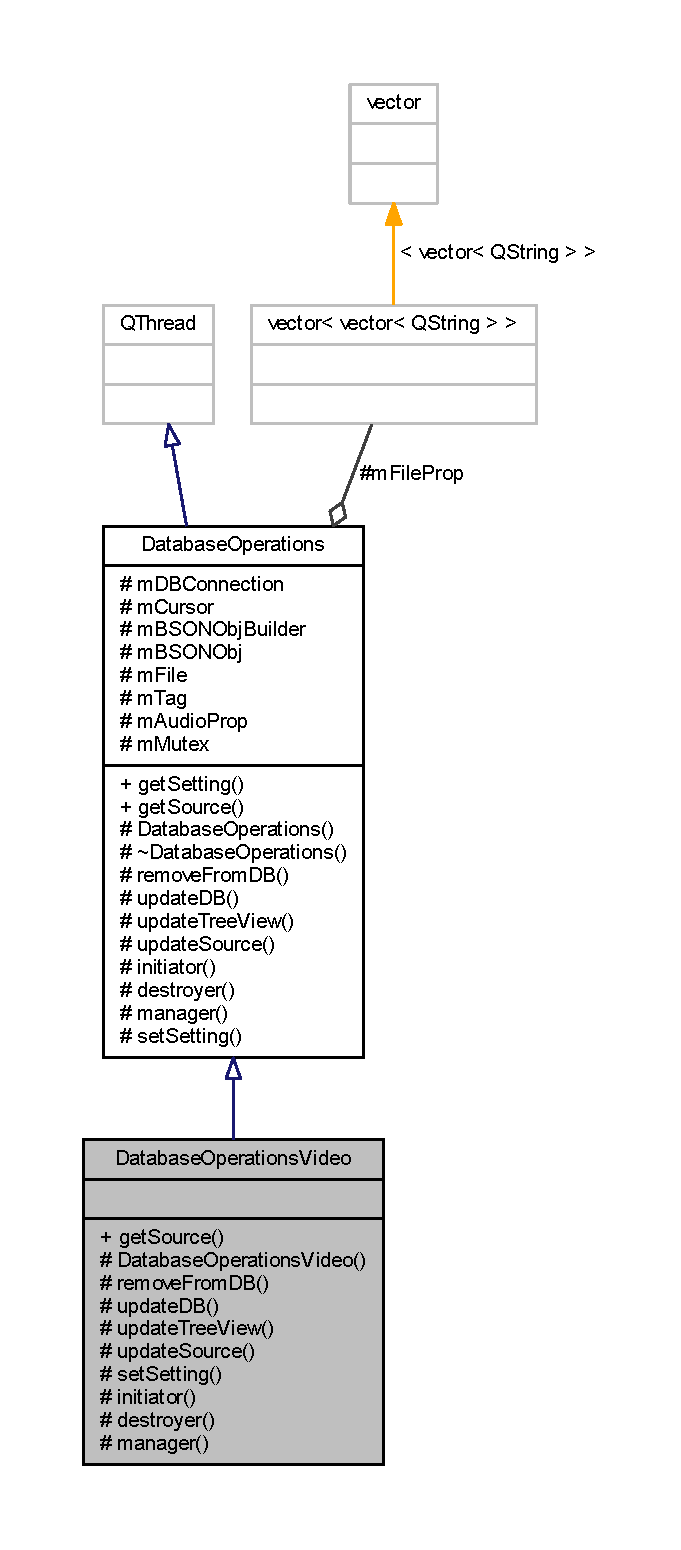
\includegraphics[height=550pt]{class_database_operations_video__coll__graph}
\end{center}
\end{figure}
\subsection*{Signals}
\begin{DoxyCompactItemize}
\item 
void \hyperlink{class_database_operations_video_a0dd4f0a7c0fb2db04227435dac72651d}{update\-Tree\-Widget\-Library\-Display} (vector$<$ vector$<$ Q\-String $>$ $>$)
\item 
void \hyperlink{class_database_operations_video_a5164513533daa6f588862c032d2412f8}{update\-Path} (Q\-String)
\end{DoxyCompactItemize}
\subsection*{Public Member Functions}
\begin{DoxyCompactItemize}
\item 
void \hyperlink{class_database_operations_video_a16849f71aa872f601c6651b43e786dab}{get\-Source} ()
\end{DoxyCompactItemize}
\subsection*{Protected Member Functions}
\begin{DoxyCompactItemize}
\item 
\hyperlink{class_database_operations_video_a319eb8b79f4f4015b2831bbf2f3c6b7b}{Database\-Operations\-Video} (Q\-Object $\ast$parent=0)
\item 
void \hyperlink{class_database_operations_video_a3187c0433cbc90c9cbcbd091bfc76e9d}{remove\-From\-D\-B} (Q\-String)
\item 
void \hyperlink{class_database_operations_video_a2e0c44a699ccc0b6248549bffe8078f9}{update\-D\-B} (Q\-String, Q\-File\-Info, Q\-File\-Info\-List)
\item 
void \hyperlink{class_database_operations_video_a958ad3432e96e3c51664bb687b244d06}{update\-Tree\-View} ()
\item 
void \hyperlink{class_database_operations_video_ac5c4d66e50e9342eede8f63d91057756}{update\-Source} (Q\-String)
\item 
void \hyperlink{class_database_operations_video_ad63d0a1dbc333e058bc910b25bbe74f4}{set\-Setting} ()
\item 
virtual void \hyperlink{class_database_operations_video_ab541cb7de9ff375af08e5e32ca1b217f}{initiator} ()=0
\item 
virtual void \hyperlink{class_database_operations_video_ab2b75036caeaa73cedc14e591d628580}{destroyer} ()=0
\item 
virtual void \hyperlink{class_database_operations_video_a54a804b782a0653e58a53c25040d3f85}{manager} ()=0
\end{DoxyCompactItemize}
\subsection*{Additional Inherited Members}


\subsection{Detailed Description}


Definition at line 6 of file databaseoperationsvideo.\-h.



\subsection{Constructor \& Destructor Documentation}
\hypertarget{class_database_operations_video_a319eb8b79f4f4015b2831bbf2f3c6b7b}{\index{Database\-Operations\-Video@{Database\-Operations\-Video}!Database\-Operations\-Video@{Database\-Operations\-Video}}
\index{Database\-Operations\-Video@{Database\-Operations\-Video}!DatabaseOperationsVideo@{Database\-Operations\-Video}}
\subsubsection[{Database\-Operations\-Video}]{\setlength{\rightskip}{0pt plus 5cm}Database\-Operations\-Video\-::\-Database\-Operations\-Video (
\begin{DoxyParamCaption}
\item[{Q\-Object $\ast$}]{parent = {\ttfamily 0}}
\end{DoxyParamCaption}
)\hspace{0.3cm}{\ttfamily [explicit]}, {\ttfamily [protected]}}}\label{class_database_operations_video_a319eb8b79f4f4015b2831bbf2f3c6b7b}


Definition at line 3 of file databaseoperationsvideo.\-cpp.



\subsection{Member Function Documentation}
\hypertarget{class_database_operations_video_ab2b75036caeaa73cedc14e591d628580}{\index{Database\-Operations\-Video@{Database\-Operations\-Video}!destroyer@{destroyer}}
\index{destroyer@{destroyer}!DatabaseOperationsVideo@{Database\-Operations\-Video}}
\subsubsection[{destroyer}]{\setlength{\rightskip}{0pt plus 5cm}virtual void Database\-Operations\-Video\-::destroyer (
\begin{DoxyParamCaption}
{}
\end{DoxyParamCaption}
)\hspace{0.3cm}{\ttfamily [protected]}, {\ttfamily [pure virtual]}}}\label{class_database_operations_video_ab2b75036caeaa73cedc14e591d628580}


Implements \hyperlink{class_database_operations_a435467e14c7ebdf3ecc6359e57c4d013}{Database\-Operations}.



Implemented in \hyperlink{class_file_finder_video_a37f0b885d2e98d3ac8b6f845c874c63d}{File\-Finder\-Video}, and \hyperlink{class_library_manager_video_abdecc35f2d907679a08f32ef8749b9bc}{Library\-Manager\-Video}.

\hypertarget{class_database_operations_video_a16849f71aa872f601c6651b43e786dab}{\index{Database\-Operations\-Video@{Database\-Operations\-Video}!get\-Source@{get\-Source}}
\index{get\-Source@{get\-Source}!DatabaseOperationsVideo@{Database\-Operations\-Video}}
\subsubsection[{get\-Source}]{\setlength{\rightskip}{0pt plus 5cm}void Database\-Operations\-Video\-::get\-Source (
\begin{DoxyParamCaption}
{}
\end{DoxyParamCaption}
)\hspace{0.3cm}{\ttfamily [virtual]}}}\label{class_database_operations_video_a16849f71aa872f601c6651b43e786dab}


Implements \hyperlink{class_database_operations_a8cf9e78c2927df5cc0a886992d394fdd}{Database\-Operations}.



Definition at line 156 of file databaseoperationsvideo.\-cpp.



Here is the caller graph for this function\-:
\nopagebreak
\begin{figure}[H]
\begin{center}
\leavevmode
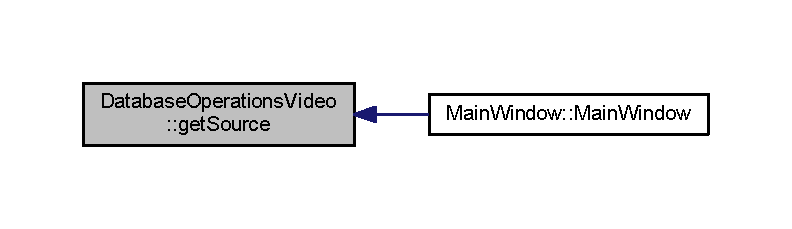
\includegraphics[width=350pt]{class_database_operations_video_a16849f71aa872f601c6651b43e786dab_icgraph}
\end{center}
\end{figure}


\hypertarget{class_database_operations_video_ab541cb7de9ff375af08e5e32ca1b217f}{\index{Database\-Operations\-Video@{Database\-Operations\-Video}!initiator@{initiator}}
\index{initiator@{initiator}!DatabaseOperationsVideo@{Database\-Operations\-Video}}
\subsubsection[{initiator}]{\setlength{\rightskip}{0pt plus 5cm}virtual void Database\-Operations\-Video\-::initiator (
\begin{DoxyParamCaption}
{}
\end{DoxyParamCaption}
)\hspace{0.3cm}{\ttfamily [protected]}, {\ttfamily [pure virtual]}}}\label{class_database_operations_video_ab541cb7de9ff375af08e5e32ca1b217f}


Implements \hyperlink{class_database_operations_af399d5ee2e6c559cf98c3ca6559f96e5}{Database\-Operations}.



Implemented in \hyperlink{class_file_finder_video_ad792218f1dafd62852f7d25bc3b80a50}{File\-Finder\-Video}.

\hypertarget{class_database_operations_video_a54a804b782a0653e58a53c25040d3f85}{\index{Database\-Operations\-Video@{Database\-Operations\-Video}!manager@{manager}}
\index{manager@{manager}!DatabaseOperationsVideo@{Database\-Operations\-Video}}
\subsubsection[{manager}]{\setlength{\rightskip}{0pt plus 5cm}virtual void Database\-Operations\-Video\-::manager (
\begin{DoxyParamCaption}
{}
\end{DoxyParamCaption}
)\hspace{0.3cm}{\ttfamily [protected]}, {\ttfamily [pure virtual]}}}\label{class_database_operations_video_a54a804b782a0653e58a53c25040d3f85}


Implements \hyperlink{class_database_operations_aeacfe0c761bf321b7a0c45763a16b4cf}{Database\-Operations}.



Implemented in \hyperlink{class_file_finder_video_aafe5126b440c0c5564a32a54fee0781c}{File\-Finder\-Video}, and \hyperlink{class_library_manager_video_a414263df76f62ab14a3372ba983cd348}{Library\-Manager\-Video}.

\hypertarget{class_database_operations_video_a3187c0433cbc90c9cbcbd091bfc76e9d}{\index{Database\-Operations\-Video@{Database\-Operations\-Video}!remove\-From\-D\-B@{remove\-From\-D\-B}}
\index{remove\-From\-D\-B@{remove\-From\-D\-B}!DatabaseOperationsVideo@{Database\-Operations\-Video}}
\subsubsection[{remove\-From\-D\-B}]{\setlength{\rightskip}{0pt plus 5cm}void Database\-Operations\-Video\-::remove\-From\-D\-B (
\begin{DoxyParamCaption}
\item[{Q\-String}]{v\-Path}
\end{DoxyParamCaption}
)\hspace{0.3cm}{\ttfamily [protected]}, {\ttfamily [virtual]}}}\label{class_database_operations_video_a3187c0433cbc90c9cbcbd091bfc76e9d}


Implements \hyperlink{class_database_operations_abab54bc65a349871c58d6027d871786e}{Database\-Operations}.



Definition at line 175 of file databaseoperationsvideo.\-cpp.



Here is the caller graph for this function\-:
\nopagebreak
\begin{figure}[H]
\begin{center}
\leavevmode
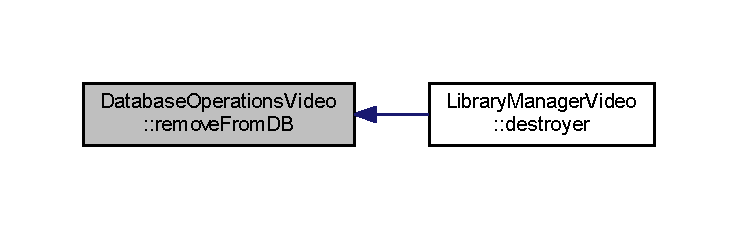
\includegraphics[width=350pt]{class_database_operations_video_a3187c0433cbc90c9cbcbd091bfc76e9d_icgraph}
\end{center}
\end{figure}


\hypertarget{class_database_operations_video_ad63d0a1dbc333e058bc910b25bbe74f4}{\index{Database\-Operations\-Video@{Database\-Operations\-Video}!set\-Setting@{set\-Setting}}
\index{set\-Setting@{set\-Setting}!DatabaseOperationsVideo@{Database\-Operations\-Video}}
\subsubsection[{set\-Setting}]{\setlength{\rightskip}{0pt plus 5cm}void Database\-Operations\-Video\-::set\-Setting (
\begin{DoxyParamCaption}
{}
\end{DoxyParamCaption}
)\hspace{0.3cm}{\ttfamily [protected]}}}\label{class_database_operations_video_ad63d0a1dbc333e058bc910b25bbe74f4}
\hypertarget{class_database_operations_video_a2e0c44a699ccc0b6248549bffe8078f9}{\index{Database\-Operations\-Video@{Database\-Operations\-Video}!update\-D\-B@{update\-D\-B}}
\index{update\-D\-B@{update\-D\-B}!DatabaseOperationsVideo@{Database\-Operations\-Video}}
\subsubsection[{update\-D\-B}]{\setlength{\rightskip}{0pt plus 5cm}void Database\-Operations\-Video\-::update\-D\-B (
\begin{DoxyParamCaption}
\item[{Q\-String}]{v\-Source, }
\item[{Q\-File\-Info}]{v\-Parent, }
\item[{Q\-File\-Info\-List}]{v\-Children}
\end{DoxyParamCaption}
)\hspace{0.3cm}{\ttfamily [protected]}, {\ttfamily [virtual]}}}\label{class_database_operations_video_a2e0c44a699ccc0b6248549bffe8078f9}


Implements \hyperlink{class_database_operations_afe6635240b49bdeb4a1cee1b948da5fd}{Database\-Operations}.



Definition at line 8 of file databaseoperationsvideo.\-cpp.



Here is the caller graph for this function\-:
\nopagebreak
\begin{figure}[H]
\begin{center}
\leavevmode
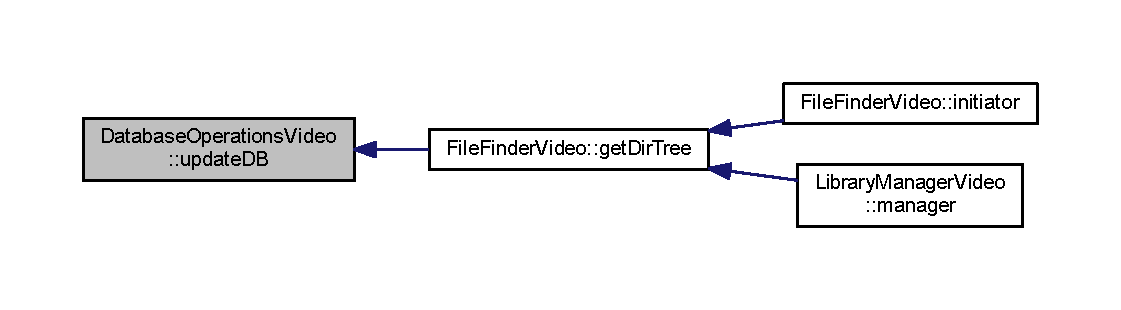
\includegraphics[width=350pt]{class_database_operations_video_a2e0c44a699ccc0b6248549bffe8078f9_icgraph}
\end{center}
\end{figure}


\hypertarget{class_database_operations_video_a5164513533daa6f588862c032d2412f8}{\index{Database\-Operations\-Video@{Database\-Operations\-Video}!update\-Path@{update\-Path}}
\index{update\-Path@{update\-Path}!DatabaseOperationsVideo@{Database\-Operations\-Video}}
\subsubsection[{update\-Path}]{\setlength{\rightskip}{0pt plus 5cm}void Database\-Operations\-Video\-::update\-Path (
\begin{DoxyParamCaption}
\item[{Q\-String}]{}
\end{DoxyParamCaption}
)\hspace{0.3cm}{\ttfamily [signal]}}}\label{class_database_operations_video_a5164513533daa6f588862c032d2412f8}


Here is the caller graph for this function\-:
\nopagebreak
\begin{figure}[H]
\begin{center}
\leavevmode
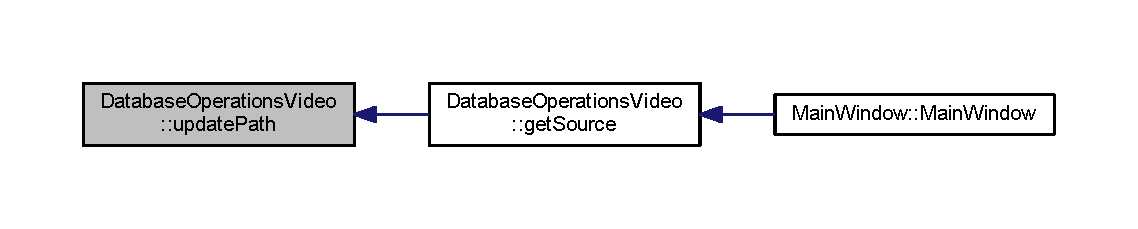
\includegraphics[width=350pt]{class_database_operations_video_a5164513533daa6f588862c032d2412f8_icgraph}
\end{center}
\end{figure}


\hypertarget{class_database_operations_video_ac5c4d66e50e9342eede8f63d91057756}{\index{Database\-Operations\-Video@{Database\-Operations\-Video}!update\-Source@{update\-Source}}
\index{update\-Source@{update\-Source}!DatabaseOperationsVideo@{Database\-Operations\-Video}}
\subsubsection[{update\-Source}]{\setlength{\rightskip}{0pt plus 5cm}void Database\-Operations\-Video\-::update\-Source (
\begin{DoxyParamCaption}
\item[{Q\-String}]{v\-Path}
\end{DoxyParamCaption}
)\hspace{0.3cm}{\ttfamily [protected]}, {\ttfamily [virtual]}}}\label{class_database_operations_video_ac5c4d66e50e9342eede8f63d91057756}


Implements \hyperlink{class_database_operations_a78b632e484e7d469f02366dbd9e1cd91}{Database\-Operations}.



Definition at line 133 of file databaseoperationsvideo.\-cpp.



Here is the caller graph for this function\-:
\nopagebreak
\begin{figure}[H]
\begin{center}
\leavevmode
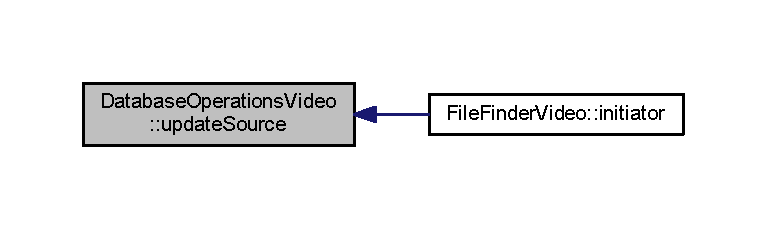
\includegraphics[width=350pt]{class_database_operations_video_ac5c4d66e50e9342eede8f63d91057756_icgraph}
\end{center}
\end{figure}


\hypertarget{class_database_operations_video_a958ad3432e96e3c51664bb687b244d06}{\index{Database\-Operations\-Video@{Database\-Operations\-Video}!update\-Tree\-View@{update\-Tree\-View}}
\index{update\-Tree\-View@{update\-Tree\-View}!DatabaseOperationsVideo@{Database\-Operations\-Video}}
\subsubsection[{update\-Tree\-View}]{\setlength{\rightskip}{0pt plus 5cm}void Database\-Operations\-Video\-::update\-Tree\-View (
\begin{DoxyParamCaption}
{}
\end{DoxyParamCaption}
)\hspace{0.3cm}{\ttfamily [protected]}, {\ttfamily [virtual]}}}\label{class_database_operations_video_a958ad3432e96e3c51664bb687b244d06}


Implements \hyperlink{class_database_operations_a77a4a371cfb8fdc2fc0cbf0f954693cd}{Database\-Operations}.



Definition at line 100 of file databaseoperationsvideo.\-cpp.



Here is the caller graph for this function\-:
\nopagebreak
\begin{figure}[H]
\begin{center}
\leavevmode
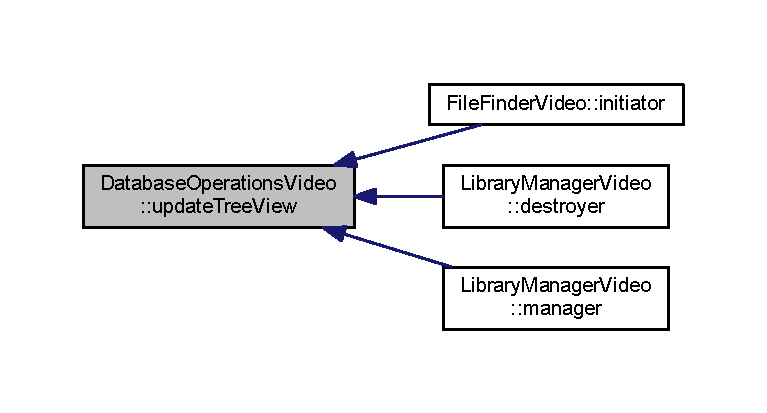
\includegraphics[width=350pt]{class_database_operations_video_a958ad3432e96e3c51664bb687b244d06_icgraph}
\end{center}
\end{figure}


\hypertarget{class_database_operations_video_a0dd4f0a7c0fb2db04227435dac72651d}{\index{Database\-Operations\-Video@{Database\-Operations\-Video}!update\-Tree\-Widget\-Library\-Display@{update\-Tree\-Widget\-Library\-Display}}
\index{update\-Tree\-Widget\-Library\-Display@{update\-Tree\-Widget\-Library\-Display}!DatabaseOperationsVideo@{Database\-Operations\-Video}}
\subsubsection[{update\-Tree\-Widget\-Library\-Display}]{\setlength{\rightskip}{0pt plus 5cm}void Database\-Operations\-Video\-::update\-Tree\-Widget\-Library\-Display (
\begin{DoxyParamCaption}
\item[{vector$<$ vector$<$ Q\-String $>$ $>$}]{}
\end{DoxyParamCaption}
)\hspace{0.3cm}{\ttfamily [signal]}}}\label{class_database_operations_video_a0dd4f0a7c0fb2db04227435dac72651d}


Here is the caller graph for this function\-:
\nopagebreak
\begin{figure}[H]
\begin{center}
\leavevmode
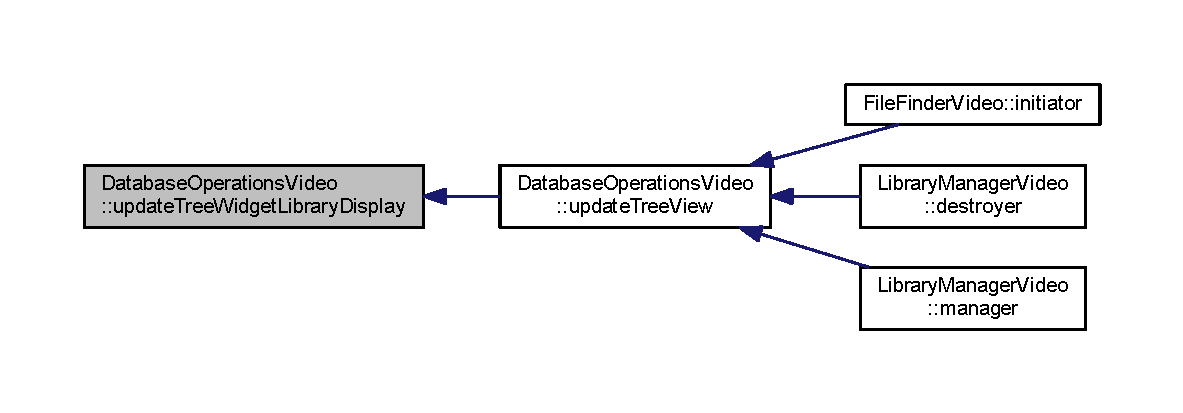
\includegraphics[width=350pt]{class_database_operations_video_a0dd4f0a7c0fb2db04227435dac72651d_icgraph}
\end{center}
\end{figure}




The documentation for this class was generated from the following files\-:\begin{DoxyCompactItemize}
\item 
C\-:/\-Users/\-X/\-Documents/\-Qt/\-Media\-Take/\hyperlink{databaseoperationsvideo_8h}{databaseoperationsvideo.\-h}\item 
C\-:/\-Users/\-X/\-Documents/\-Qt/\-Media\-Take/\hyperlink{databaseoperationsvideo_8cpp}{databaseoperationsvideo.\-cpp}\end{DoxyCompactItemize}

\hypertarget{class_file_finder_audio}{\section{File\-Finder\-Audio Class Reference}
\label{class_file_finder_audio}\index{File\-Finder\-Audio@{File\-Finder\-Audio}}
}


{\ttfamily \#include $<$filefinderaudio.\-h$>$}



Inheritance diagram for File\-Finder\-Audio\-:
\nopagebreak
\begin{figure}[H]
\begin{center}
\leavevmode
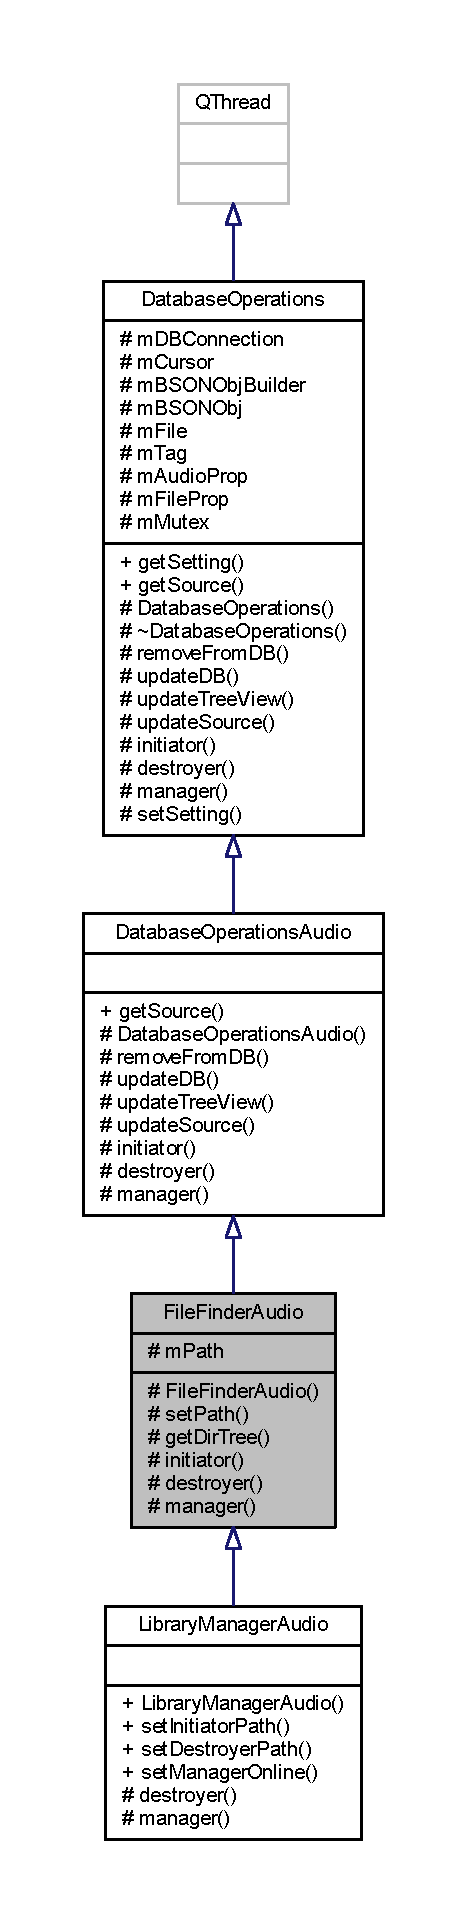
\includegraphics[height=550pt]{class_file_finder_audio__inherit__graph}
\end{center}
\end{figure}


Collaboration diagram for File\-Finder\-Audio\-:
\nopagebreak
\begin{figure}[H]
\begin{center}
\leavevmode
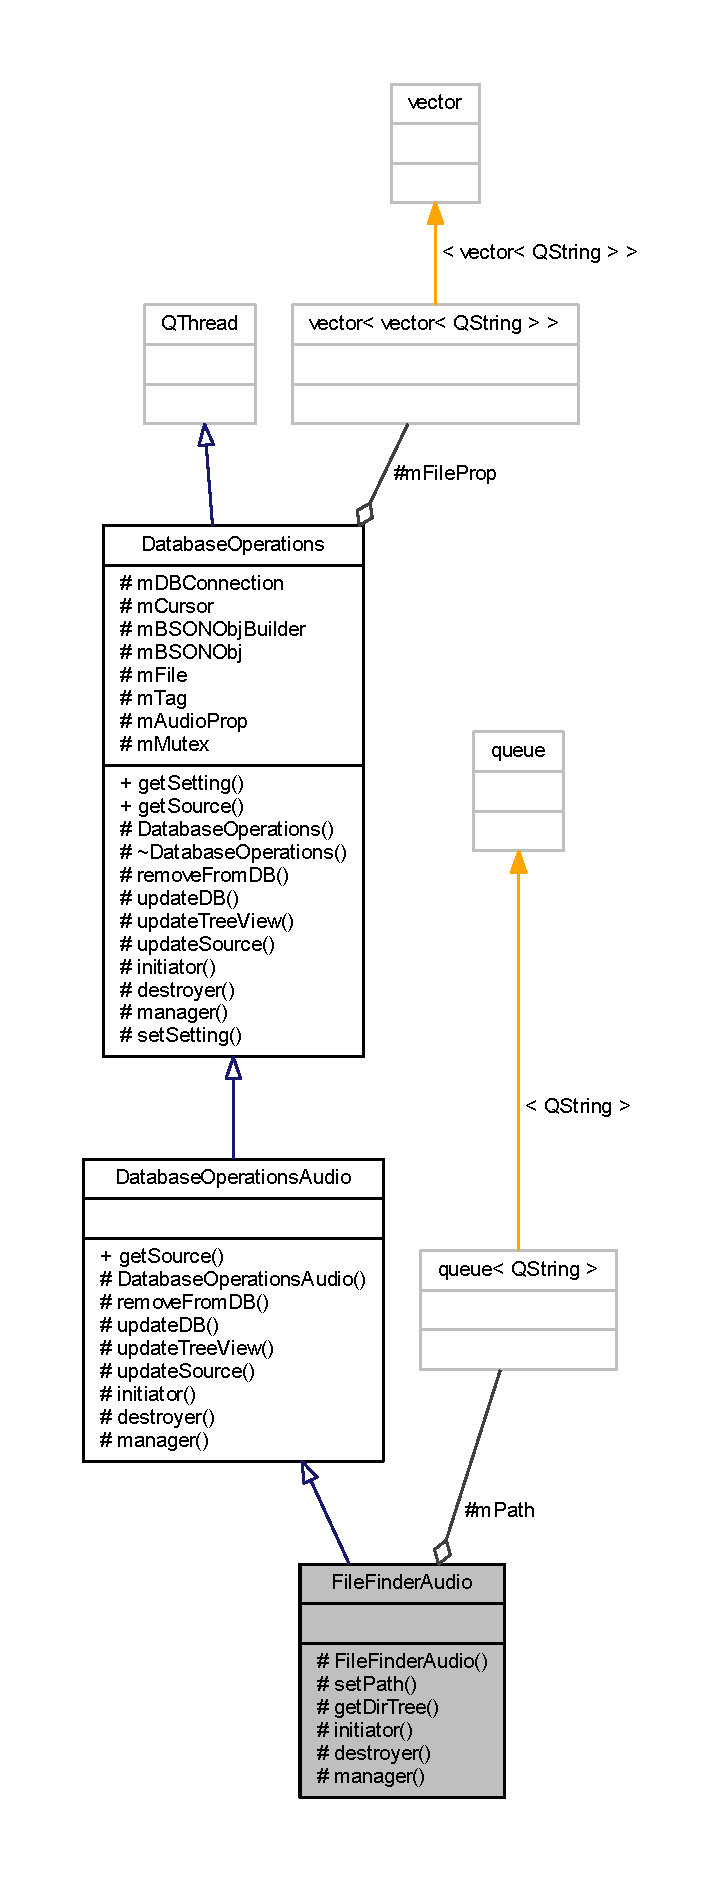
\includegraphics[height=550pt]{class_file_finder_audio__coll__graph}
\end{center}
\end{figure}
\subsection*{Protected Member Functions}
\begin{DoxyCompactItemize}
\item 
\hyperlink{class_file_finder_audio_ac55cb6b9449535fa894bf28b676c5d90}{File\-Finder\-Audio} (Q\-Object $\ast$parent=0)
\item 
void \hyperlink{class_file_finder_audio_a75465aa7c289474f155d1e20acb23e65}{set\-Path} (Q\-String)
\item 
void \hyperlink{class_file_finder_audio_a7d590d88a79ee9327c86761ce1f6e89b}{get\-Dir\-Tree} ()
\item 
void \hyperlink{class_file_finder_audio_af8153dd34e8691aab1445413b3a86d12}{initiator} ()
\item 
virtual void \hyperlink{class_file_finder_audio_aeab95a78219b1fb187da1cae16a6b9c8}{destroyer} ()=0
\item 
virtual void \hyperlink{class_file_finder_audio_ab11c9010b5031e4e251e2fe592ea6321}{manager} ()=0
\end{DoxyCompactItemize}
\subsection*{Protected Attributes}
\begin{DoxyCompactItemize}
\item 
queue$<$ Q\-String $>$ \hyperlink{class_file_finder_audio_a3a01ab7a81d46a6f15667476cc4ee71a}{m\-Path}
\end{DoxyCompactItemize}
\subsection*{Additional Inherited Members}


\subsection{Detailed Description}


Definition at line 11 of file filefinderaudio.\-h.



\subsection{Constructor \& Destructor Documentation}
\hypertarget{class_file_finder_audio_ac55cb6b9449535fa894bf28b676c5d90}{\index{File\-Finder\-Audio@{File\-Finder\-Audio}!File\-Finder\-Audio@{File\-Finder\-Audio}}
\index{File\-Finder\-Audio@{File\-Finder\-Audio}!FileFinderAudio@{File\-Finder\-Audio}}
\subsubsection[{File\-Finder\-Audio}]{\setlength{\rightskip}{0pt plus 5cm}File\-Finder\-Audio\-::\-File\-Finder\-Audio (
\begin{DoxyParamCaption}
\item[{Q\-Object $\ast$}]{parent = {\ttfamily 0}}
\end{DoxyParamCaption}
)\hspace{0.3cm}{\ttfamily [explicit]}, {\ttfamily [protected]}}}\label{class_file_finder_audio_ac55cb6b9449535fa894bf28b676c5d90}


Definition at line 3 of file filefinderaudio.\-cpp.



\subsection{Member Function Documentation}
\hypertarget{class_file_finder_audio_aeab95a78219b1fb187da1cae16a6b9c8}{\index{File\-Finder\-Audio@{File\-Finder\-Audio}!destroyer@{destroyer}}
\index{destroyer@{destroyer}!FileFinderAudio@{File\-Finder\-Audio}}
\subsubsection[{destroyer}]{\setlength{\rightskip}{0pt plus 5cm}virtual void File\-Finder\-Audio\-::destroyer (
\begin{DoxyParamCaption}
{}
\end{DoxyParamCaption}
)\hspace{0.3cm}{\ttfamily [protected]}, {\ttfamily [pure virtual]}}}\label{class_file_finder_audio_aeab95a78219b1fb187da1cae16a6b9c8}


Implements \hyperlink{class_database_operations_audio_ab4879167601725f2faf7a69d73aa2309}{Database\-Operations\-Audio}.



Implemented in \hyperlink{class_library_manager_audio_af69df97c95e9e0fae6b08d071b9ab93d}{Library\-Manager\-Audio}.

\hypertarget{class_file_finder_audio_a7d590d88a79ee9327c86761ce1f6e89b}{\index{File\-Finder\-Audio@{File\-Finder\-Audio}!get\-Dir\-Tree@{get\-Dir\-Tree}}
\index{get\-Dir\-Tree@{get\-Dir\-Tree}!FileFinderAudio@{File\-Finder\-Audio}}
\subsubsection[{get\-Dir\-Tree}]{\setlength{\rightskip}{0pt plus 5cm}void File\-Finder\-Audio\-::get\-Dir\-Tree (
\begin{DoxyParamCaption}
{}
\end{DoxyParamCaption}
)\hspace{0.3cm}{\ttfamily [protected]}}}\label{class_file_finder_audio_a7d590d88a79ee9327c86761ce1f6e89b}


Definition at line 8 of file filefinderaudio.\-cpp.



Here is the call graph for this function\-:
\nopagebreak
\begin{figure}[H]
\begin{center}
\leavevmode
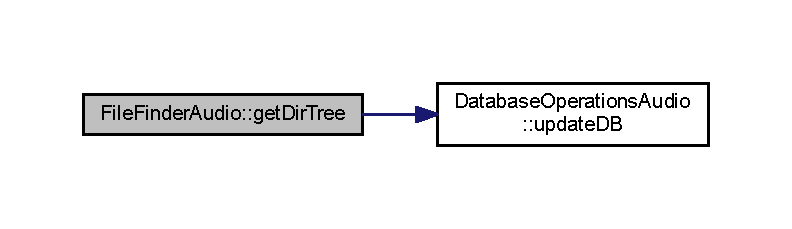
\includegraphics[width=350pt]{class_file_finder_audio_a7d590d88a79ee9327c86761ce1f6e89b_cgraph}
\end{center}
\end{figure}




Here is the caller graph for this function\-:
\nopagebreak
\begin{figure}[H]
\begin{center}
\leavevmode
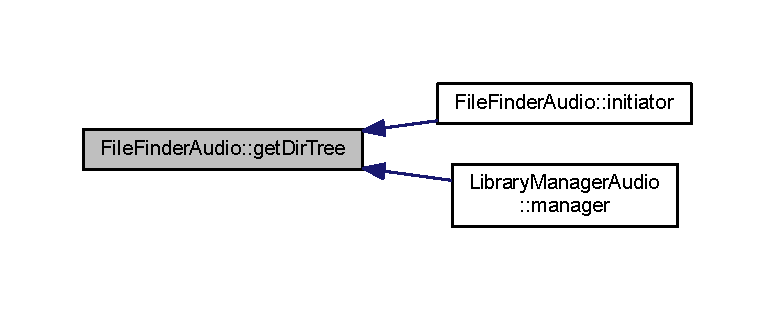
\includegraphics[width=350pt]{class_file_finder_audio_a7d590d88a79ee9327c86761ce1f6e89b_icgraph}
\end{center}
\end{figure}


\hypertarget{class_file_finder_audio_af8153dd34e8691aab1445413b3a86d12}{\index{File\-Finder\-Audio@{File\-Finder\-Audio}!initiator@{initiator}}
\index{initiator@{initiator}!FileFinderAudio@{File\-Finder\-Audio}}
\subsubsection[{initiator}]{\setlength{\rightskip}{0pt plus 5cm}void File\-Finder\-Audio\-::initiator (
\begin{DoxyParamCaption}
{}
\end{DoxyParamCaption}
)\hspace{0.3cm}{\ttfamily [protected]}, {\ttfamily [virtual]}}}\label{class_file_finder_audio_af8153dd34e8691aab1445413b3a86d12}


Implements \hyperlink{class_database_operations_audio_a80507c96dabef6ca3a06a0d3f83fb657}{Database\-Operations\-Audio}.



Definition at line 75 of file filefinderaudio.\-cpp.



Here is the call graph for this function\-:
\nopagebreak
\begin{figure}[H]
\begin{center}
\leavevmode
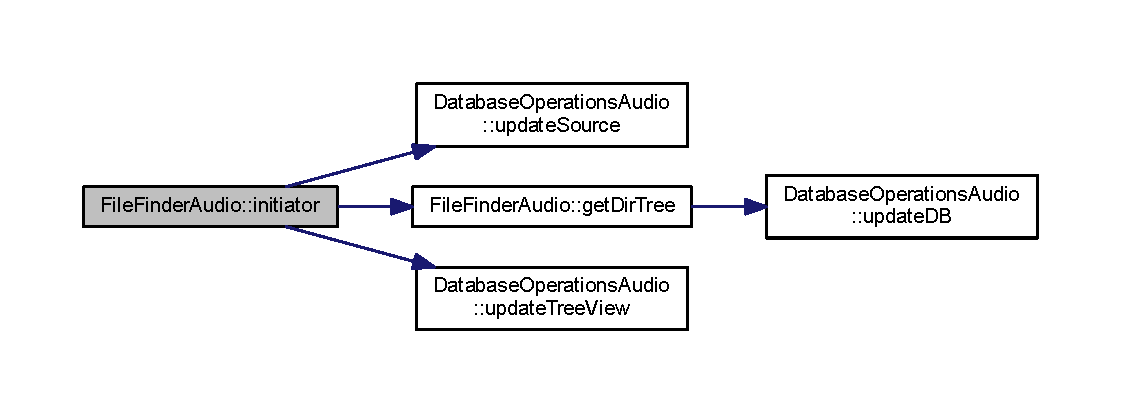
\includegraphics[width=350pt]{class_file_finder_audio_af8153dd34e8691aab1445413b3a86d12_cgraph}
\end{center}
\end{figure}


\hypertarget{class_file_finder_audio_ab11c9010b5031e4e251e2fe592ea6321}{\index{File\-Finder\-Audio@{File\-Finder\-Audio}!manager@{manager}}
\index{manager@{manager}!FileFinderAudio@{File\-Finder\-Audio}}
\subsubsection[{manager}]{\setlength{\rightskip}{0pt plus 5cm}virtual void File\-Finder\-Audio\-::manager (
\begin{DoxyParamCaption}
{}
\end{DoxyParamCaption}
)\hspace{0.3cm}{\ttfamily [protected]}, {\ttfamily [pure virtual]}}}\label{class_file_finder_audio_ab11c9010b5031e4e251e2fe592ea6321}


Implements \hyperlink{class_database_operations_audio_a7db082335a6a48ce277383f5382c15c2}{Database\-Operations\-Audio}.



Implemented in \hyperlink{class_library_manager_audio_ad2176013457295b02726edb2e6a547c4}{Library\-Manager\-Audio}.

\hypertarget{class_file_finder_audio_a75465aa7c289474f155d1e20acb23e65}{\index{File\-Finder\-Audio@{File\-Finder\-Audio}!set\-Path@{set\-Path}}
\index{set\-Path@{set\-Path}!FileFinderAudio@{File\-Finder\-Audio}}
\subsubsection[{set\-Path}]{\setlength{\rightskip}{0pt plus 5cm}void File\-Finder\-Audio\-::set\-Path (
\begin{DoxyParamCaption}
\item[{Q\-String}]{v\-Path}
\end{DoxyParamCaption}
)\hspace{0.3cm}{\ttfamily [protected]}}}\label{class_file_finder_audio_a75465aa7c289474f155d1e20acb23e65}


Definition at line 70 of file filefinderaudio.\-cpp.



Here is the caller graph for this function\-:
\nopagebreak
\begin{figure}[H]
\begin{center}
\leavevmode
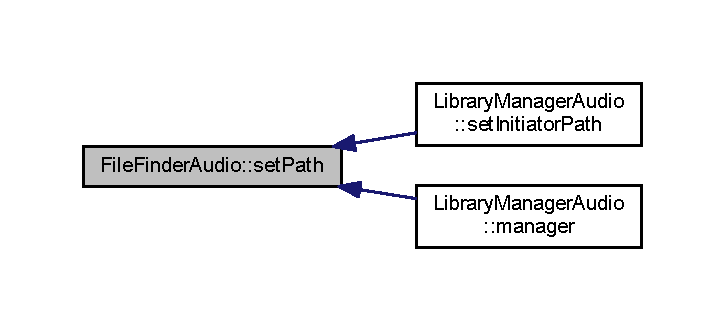
\includegraphics[width=348pt]{class_file_finder_audio_a75465aa7c289474f155d1e20acb23e65_icgraph}
\end{center}
\end{figure}




\subsection{Member Data Documentation}
\hypertarget{class_file_finder_audio_a3a01ab7a81d46a6f15667476cc4ee71a}{\index{File\-Finder\-Audio@{File\-Finder\-Audio}!m\-Path@{m\-Path}}
\index{m\-Path@{m\-Path}!FileFinderAudio@{File\-Finder\-Audio}}
\subsubsection[{m\-Path}]{\setlength{\rightskip}{0pt plus 5cm}queue$<$Q\-String$>$ File\-Finder\-Audio\-::m\-Path\hspace{0.3cm}{\ttfamily [protected]}}}\label{class_file_finder_audio_a3a01ab7a81d46a6f15667476cc4ee71a}


Definition at line 23 of file filefinderaudio.\-h.



The documentation for this class was generated from the following files\-:\begin{DoxyCompactItemize}
\item 
C\-:/\-Users/\-X/\-Documents/\-Qt/\-Media\-Take/\hyperlink{filefinderaudio_8h}{filefinderaudio.\-h}\item 
C\-:/\-Users/\-X/\-Documents/\-Qt/\-Media\-Take/\hyperlink{filefinderaudio_8cpp}{filefinderaudio.\-cpp}\end{DoxyCompactItemize}

\hypertarget{class_file_finder_video}{\section{File\-Finder\-Video Class Reference}
\label{class_file_finder_video}\index{File\-Finder\-Video@{File\-Finder\-Video}}
}


{\ttfamily \#include $<$filefindervideo.\-h$>$}



Inheritance diagram for File\-Finder\-Video\-:
\nopagebreak
\begin{figure}[H]
\begin{center}
\leavevmode
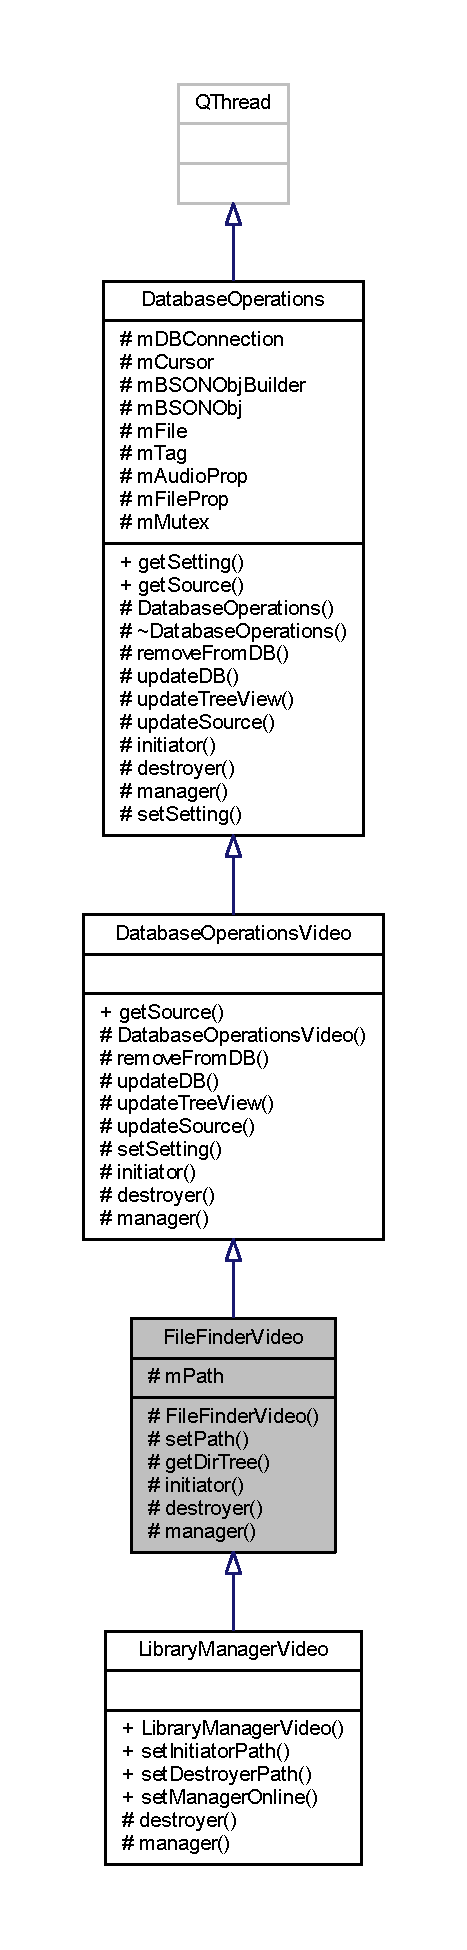
\includegraphics[height=550pt]{class_file_finder_video__inherit__graph}
\end{center}
\end{figure}


Collaboration diagram for File\-Finder\-Video\-:
\nopagebreak
\begin{figure}[H]
\begin{center}
\leavevmode
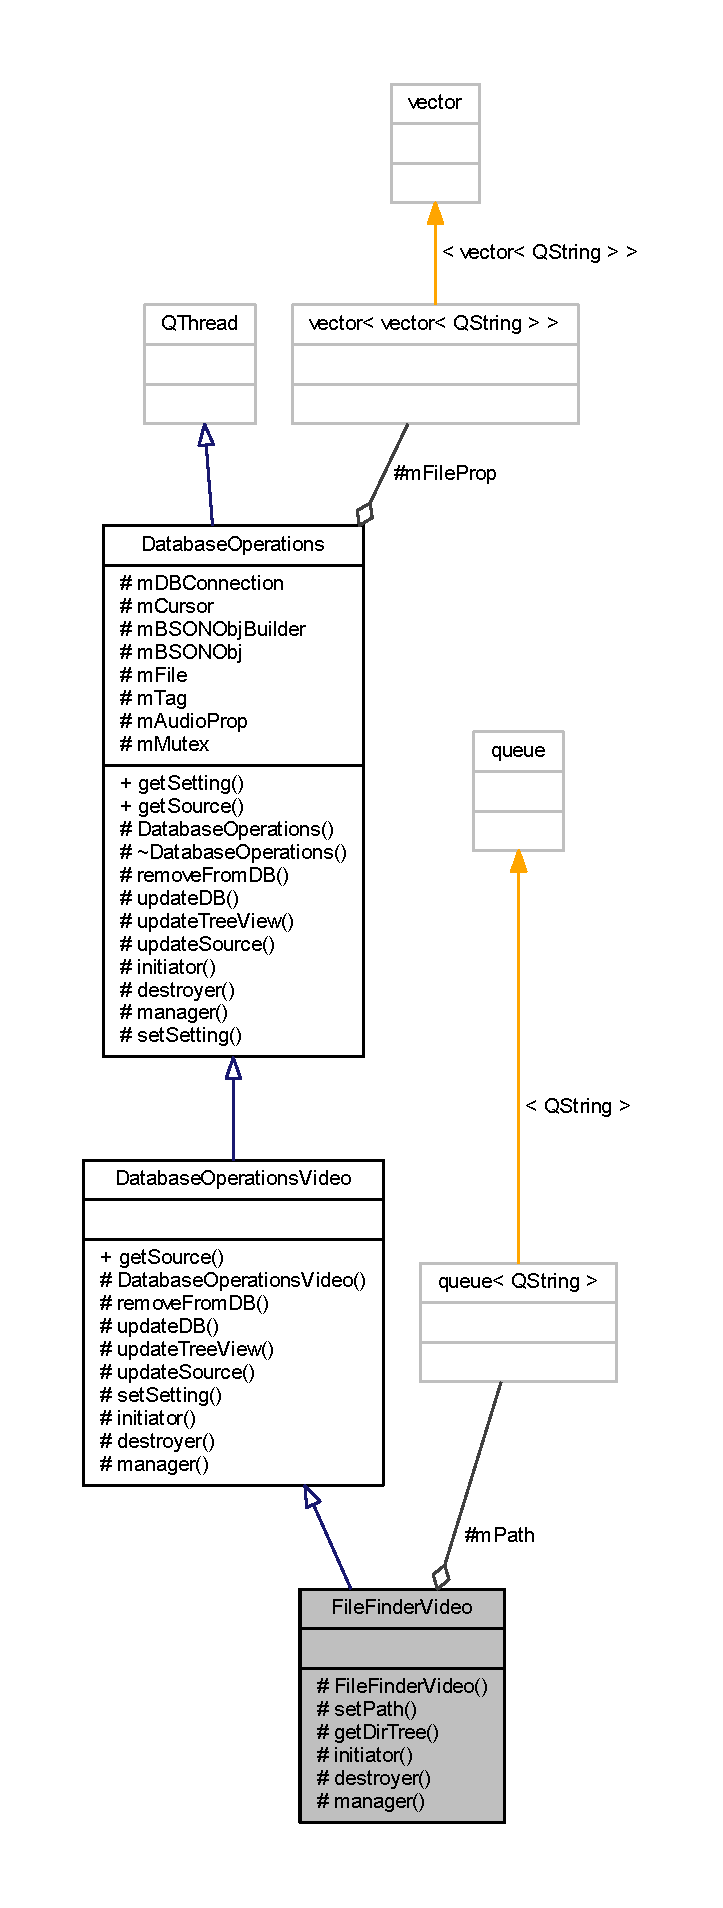
\includegraphics[height=550pt]{class_file_finder_video__coll__graph}
\end{center}
\end{figure}
\subsection*{Protected Member Functions}
\begin{DoxyCompactItemize}
\item 
\hyperlink{class_file_finder_video_a090fd7eb7d99d7f018523c87548d6b8e}{File\-Finder\-Video} (Q\-Object $\ast$parent=0)
\item 
void \hyperlink{class_file_finder_video_aa0711fca668fcc1e06b603d330f4bf8c}{set\-Path} (Q\-String)
\item 
void \hyperlink{class_file_finder_video_a9865b680e146d66acf9616f8f5f70db6}{get\-Dir\-Tree} ()
\item 
void \hyperlink{class_file_finder_video_ad792218f1dafd62852f7d25bc3b80a50}{initiator} ()
\item 
virtual void \hyperlink{class_file_finder_video_a37f0b885d2e98d3ac8b6f845c874c63d}{destroyer} ()=0
\item 
virtual void \hyperlink{class_file_finder_video_aafe5126b440c0c5564a32a54fee0781c}{manager} ()=0
\end{DoxyCompactItemize}
\subsection*{Protected Attributes}
\begin{DoxyCompactItemize}
\item 
queue$<$ Q\-String $>$ \hyperlink{class_file_finder_video_a1b7ea45f53c63b4ca04f545a04aafe99}{m\-Path}
\end{DoxyCompactItemize}
\subsection*{Additional Inherited Members}


\subsection{Detailed Description}


Definition at line 10 of file filefindervideo.\-h.



\subsection{Constructor \& Destructor Documentation}
\hypertarget{class_file_finder_video_a090fd7eb7d99d7f018523c87548d6b8e}{\index{File\-Finder\-Video@{File\-Finder\-Video}!File\-Finder\-Video@{File\-Finder\-Video}}
\index{File\-Finder\-Video@{File\-Finder\-Video}!FileFinderVideo@{File\-Finder\-Video}}
\subsubsection[{File\-Finder\-Video}]{\setlength{\rightskip}{0pt plus 5cm}File\-Finder\-Video\-::\-File\-Finder\-Video (
\begin{DoxyParamCaption}
\item[{Q\-Object $\ast$}]{parent = {\ttfamily 0}}
\end{DoxyParamCaption}
)\hspace{0.3cm}{\ttfamily [explicit]}, {\ttfamily [protected]}}}\label{class_file_finder_video_a090fd7eb7d99d7f018523c87548d6b8e}


Definition at line 3 of file filefindervideo.\-cpp.



\subsection{Member Function Documentation}
\hypertarget{class_file_finder_video_a37f0b885d2e98d3ac8b6f845c874c63d}{\index{File\-Finder\-Video@{File\-Finder\-Video}!destroyer@{destroyer}}
\index{destroyer@{destroyer}!FileFinderVideo@{File\-Finder\-Video}}
\subsubsection[{destroyer}]{\setlength{\rightskip}{0pt plus 5cm}virtual void File\-Finder\-Video\-::destroyer (
\begin{DoxyParamCaption}
{}
\end{DoxyParamCaption}
)\hspace{0.3cm}{\ttfamily [protected]}, {\ttfamily [pure virtual]}}}\label{class_file_finder_video_a37f0b885d2e98d3ac8b6f845c874c63d}


Implements \hyperlink{class_database_operations_video_ab2b75036caeaa73cedc14e591d628580}{Database\-Operations\-Video}.



Implemented in \hyperlink{class_library_manager_video_abdecc35f2d907679a08f32ef8749b9bc}{Library\-Manager\-Video}.

\hypertarget{class_file_finder_video_a9865b680e146d66acf9616f8f5f70db6}{\index{File\-Finder\-Video@{File\-Finder\-Video}!get\-Dir\-Tree@{get\-Dir\-Tree}}
\index{get\-Dir\-Tree@{get\-Dir\-Tree}!FileFinderVideo@{File\-Finder\-Video}}
\subsubsection[{get\-Dir\-Tree}]{\setlength{\rightskip}{0pt plus 5cm}void File\-Finder\-Video\-::get\-Dir\-Tree (
\begin{DoxyParamCaption}
{}
\end{DoxyParamCaption}
)\hspace{0.3cm}{\ttfamily [protected]}}}\label{class_file_finder_video_a9865b680e146d66acf9616f8f5f70db6}


Definition at line 9 of file filefindervideo.\-cpp.



Here is the call graph for this function\-:
\nopagebreak
\begin{figure}[H]
\begin{center}
\leavevmode
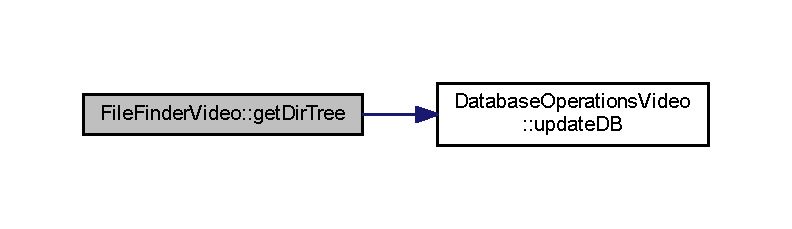
\includegraphics[width=350pt]{class_file_finder_video_a9865b680e146d66acf9616f8f5f70db6_cgraph}
\end{center}
\end{figure}




Here is the caller graph for this function\-:
\nopagebreak
\begin{figure}[H]
\begin{center}
\leavevmode
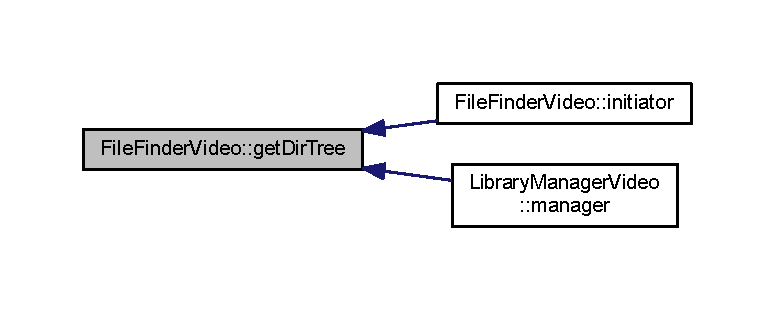
\includegraphics[width=350pt]{class_file_finder_video_a9865b680e146d66acf9616f8f5f70db6_icgraph}
\end{center}
\end{figure}


\hypertarget{class_file_finder_video_ad792218f1dafd62852f7d25bc3b80a50}{\index{File\-Finder\-Video@{File\-Finder\-Video}!initiator@{initiator}}
\index{initiator@{initiator}!FileFinderVideo@{File\-Finder\-Video}}
\subsubsection[{initiator}]{\setlength{\rightskip}{0pt plus 5cm}void File\-Finder\-Video\-::initiator (
\begin{DoxyParamCaption}
{}
\end{DoxyParamCaption}
)\hspace{0.3cm}{\ttfamily [protected]}, {\ttfamily [virtual]}}}\label{class_file_finder_video_ad792218f1dafd62852f7d25bc3b80a50}


Implements \hyperlink{class_database_operations_video_ab541cb7de9ff375af08e5e32ca1b217f}{Database\-Operations\-Video}.



Definition at line 80 of file filefindervideo.\-cpp.



Here is the call graph for this function\-:
\nopagebreak
\begin{figure}[H]
\begin{center}
\leavevmode
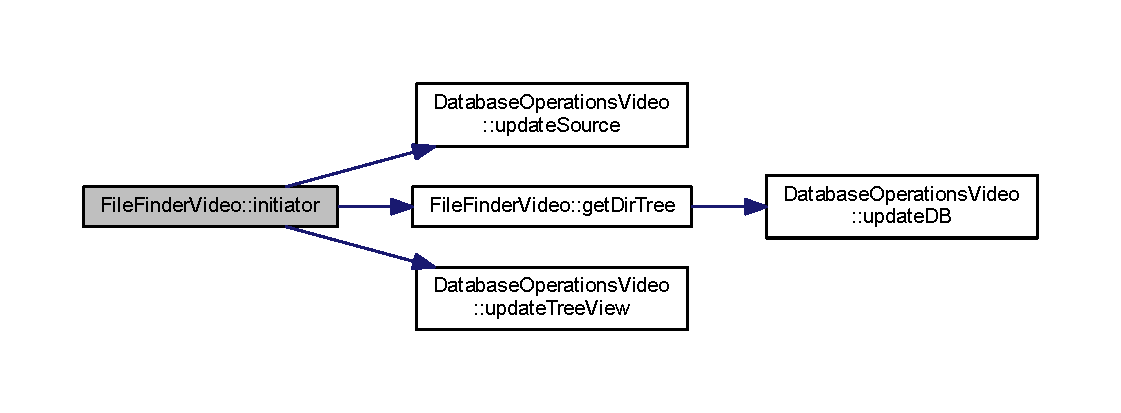
\includegraphics[width=350pt]{class_file_finder_video_ad792218f1dafd62852f7d25bc3b80a50_cgraph}
\end{center}
\end{figure}


\hypertarget{class_file_finder_video_aafe5126b440c0c5564a32a54fee0781c}{\index{File\-Finder\-Video@{File\-Finder\-Video}!manager@{manager}}
\index{manager@{manager}!FileFinderVideo@{File\-Finder\-Video}}
\subsubsection[{manager}]{\setlength{\rightskip}{0pt plus 5cm}virtual void File\-Finder\-Video\-::manager (
\begin{DoxyParamCaption}
{}
\end{DoxyParamCaption}
)\hspace{0.3cm}{\ttfamily [protected]}, {\ttfamily [pure virtual]}}}\label{class_file_finder_video_aafe5126b440c0c5564a32a54fee0781c}


Implements \hyperlink{class_database_operations_video_a54a804b782a0653e58a53c25040d3f85}{Database\-Operations\-Video}.



Implemented in \hyperlink{class_library_manager_video_a414263df76f62ab14a3372ba983cd348}{Library\-Manager\-Video}.

\hypertarget{class_file_finder_video_aa0711fca668fcc1e06b603d330f4bf8c}{\index{File\-Finder\-Video@{File\-Finder\-Video}!set\-Path@{set\-Path}}
\index{set\-Path@{set\-Path}!FileFinderVideo@{File\-Finder\-Video}}
\subsubsection[{set\-Path}]{\setlength{\rightskip}{0pt plus 5cm}void File\-Finder\-Video\-::set\-Path (
\begin{DoxyParamCaption}
\item[{Q\-String}]{v\-Path}
\end{DoxyParamCaption}
)\hspace{0.3cm}{\ttfamily [protected]}}}\label{class_file_finder_video_aa0711fca668fcc1e06b603d330f4bf8c}


Definition at line 75 of file filefindervideo.\-cpp.



Here is the caller graph for this function\-:
\nopagebreak
\begin{figure}[H]
\begin{center}
\leavevmode
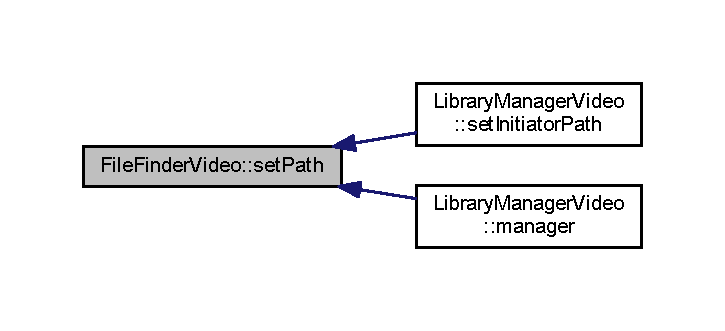
\includegraphics[width=348pt]{class_file_finder_video_aa0711fca668fcc1e06b603d330f4bf8c_icgraph}
\end{center}
\end{figure}




\subsection{Member Data Documentation}
\hypertarget{class_file_finder_video_a1b7ea45f53c63b4ca04f545a04aafe99}{\index{File\-Finder\-Video@{File\-Finder\-Video}!m\-Path@{m\-Path}}
\index{m\-Path@{m\-Path}!FileFinderVideo@{File\-Finder\-Video}}
\subsubsection[{m\-Path}]{\setlength{\rightskip}{0pt plus 5cm}queue$<$Q\-String$>$ File\-Finder\-Video\-::m\-Path\hspace{0.3cm}{\ttfamily [protected]}}}\label{class_file_finder_video_a1b7ea45f53c63b4ca04f545a04aafe99}


Definition at line 21 of file filefindervideo.\-h.



The documentation for this class was generated from the following files\-:\begin{DoxyCompactItemize}
\item 
C\-:/\-Users/\-X/\-Documents/\-Qt/\-Media\-Take/\hyperlink{filefindervideo_8h}{filefindervideo.\-h}\item 
C\-:/\-Users/\-X/\-Documents/\-Qt/\-Media\-Take/\hyperlink{filefindervideo_8cpp}{filefindervideo.\-cpp}\end{DoxyCompactItemize}

\hypertarget{class_library_manager_audio}{\section{Library\-Manager\-Audio Class Reference}
\label{class_library_manager_audio}\index{Library\-Manager\-Audio@{Library\-Manager\-Audio}}
}


{\ttfamily \#include $<$librarymanageraudio.\-h$>$}



Inheritance diagram for Library\-Manager\-Audio\-:
\nopagebreak
\begin{figure}[H]
\begin{center}
\leavevmode
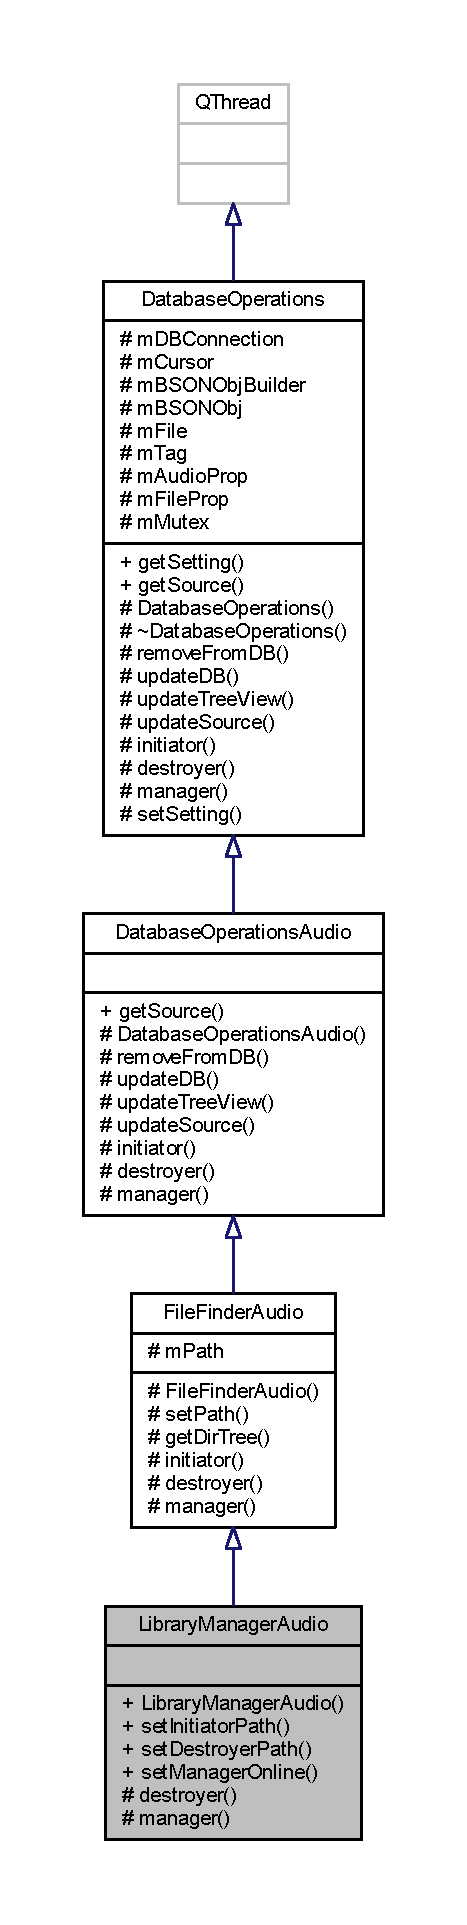
\includegraphics[height=550pt]{class_library_manager_audio__inherit__graph}
\end{center}
\end{figure}


Collaboration diagram for Library\-Manager\-Audio\-:
\nopagebreak
\begin{figure}[H]
\begin{center}
\leavevmode
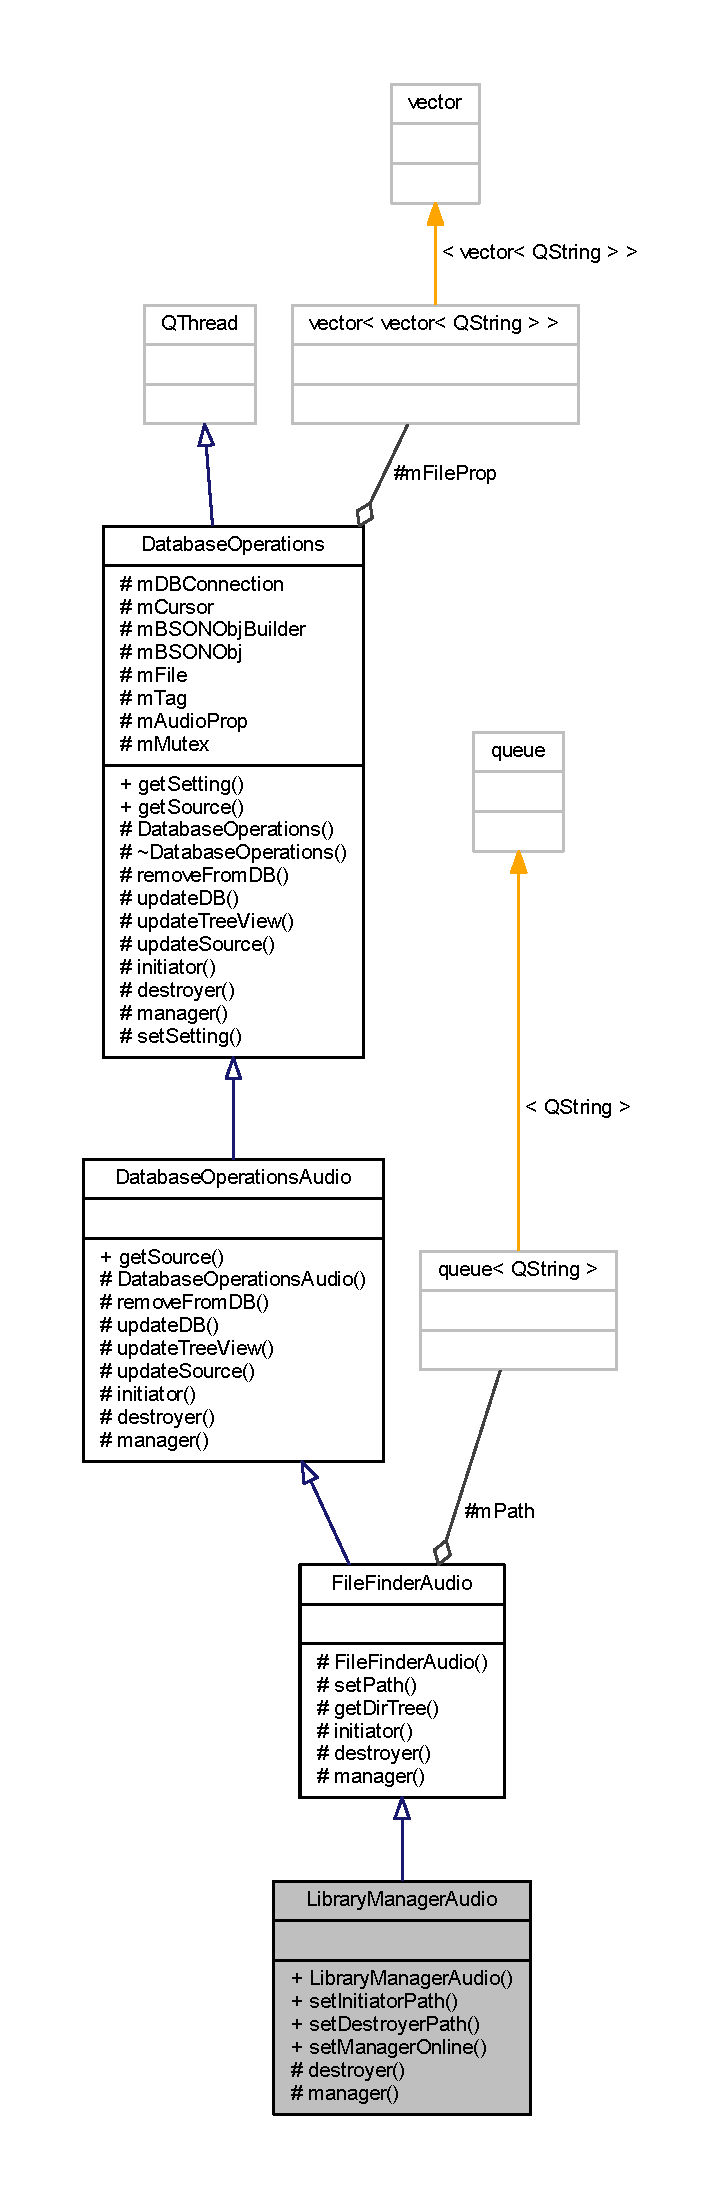
\includegraphics[height=550pt]{class_library_manager_audio__coll__graph}
\end{center}
\end{figure}
\subsection*{Public Member Functions}
\begin{DoxyCompactItemize}
\item 
\hyperlink{class_library_manager_audio_a8d54634f0bbf37a513a74ca37f753777}{Library\-Manager\-Audio} (Q\-Object $\ast$parent=0)
\item 
void \hyperlink{class_library_manager_audio_a3f71d69d66a6b666e02171349950ee8a}{set\-Initiator\-Path} (Q\-String)
\item 
void \hyperlink{class_library_manager_audio_a5c1d68b8e484b208dbf43aaf97807e69}{set\-Destroyer\-Path} (Q\-String)
\item 
void \hyperlink{class_library_manager_audio_aeeb16a8820789dcd1680331707c7c72e}{set\-Manager\-Online} ()
\end{DoxyCompactItemize}
\subsection*{Protected Member Functions}
\begin{DoxyCompactItemize}
\item 
void \hyperlink{class_library_manager_audio_af69df97c95e9e0fae6b08d071b9ab93d}{destroyer} ()
\item 
void \hyperlink{class_library_manager_audio_ad2176013457295b02726edb2e6a547c4}{manager} ()
\end{DoxyCompactItemize}
\subsection*{Additional Inherited Members}


\subsection{Detailed Description}


Definition at line 11 of file librarymanageraudio.\-h.



\subsection{Constructor \& Destructor Documentation}
\hypertarget{class_library_manager_audio_a8d54634f0bbf37a513a74ca37f753777}{\index{Library\-Manager\-Audio@{Library\-Manager\-Audio}!Library\-Manager\-Audio@{Library\-Manager\-Audio}}
\index{Library\-Manager\-Audio@{Library\-Manager\-Audio}!LibraryManagerAudio@{Library\-Manager\-Audio}}
\subsubsection[{Library\-Manager\-Audio}]{\setlength{\rightskip}{0pt plus 5cm}Library\-Manager\-Audio\-::\-Library\-Manager\-Audio (
\begin{DoxyParamCaption}
\item[{Q\-Object $\ast$}]{parent = {\ttfamily 0}}
\end{DoxyParamCaption}
)\hspace{0.3cm}{\ttfamily [explicit]}}}\label{class_library_manager_audio_a8d54634f0bbf37a513a74ca37f753777}


Definition at line 3 of file librarymanageraudio.\-cpp.



\subsection{Member Function Documentation}
\hypertarget{class_library_manager_audio_af69df97c95e9e0fae6b08d071b9ab93d}{\index{Library\-Manager\-Audio@{Library\-Manager\-Audio}!destroyer@{destroyer}}
\index{destroyer@{destroyer}!LibraryManagerAudio@{Library\-Manager\-Audio}}
\subsubsection[{destroyer}]{\setlength{\rightskip}{0pt plus 5cm}void Library\-Manager\-Audio\-::destroyer (
\begin{DoxyParamCaption}
{}
\end{DoxyParamCaption}
)\hspace{0.3cm}{\ttfamily [protected]}, {\ttfamily [virtual]}}}\label{class_library_manager_audio_af69df97c95e9e0fae6b08d071b9ab93d}


Implements \hyperlink{class_file_finder_audio_aeab95a78219b1fb187da1cae16a6b9c8}{File\-Finder\-Audio}.



Definition at line 39 of file librarymanageraudio.\-cpp.



Here is the call graph for this function\-:
\nopagebreak
\begin{figure}[H]
\begin{center}
\leavevmode
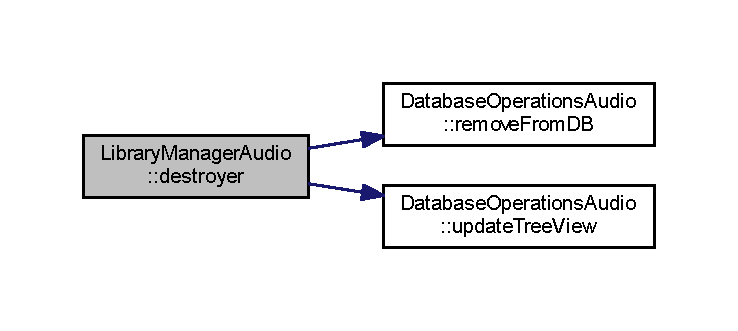
\includegraphics[width=350pt]{class_library_manager_audio_af69df97c95e9e0fae6b08d071b9ab93d_cgraph}
\end{center}
\end{figure}


\hypertarget{class_library_manager_audio_ad2176013457295b02726edb2e6a547c4}{\index{Library\-Manager\-Audio@{Library\-Manager\-Audio}!manager@{manager}}
\index{manager@{manager}!LibraryManagerAudio@{Library\-Manager\-Audio}}
\subsubsection[{manager}]{\setlength{\rightskip}{0pt plus 5cm}void Library\-Manager\-Audio\-::manager (
\begin{DoxyParamCaption}
{}
\end{DoxyParamCaption}
)\hspace{0.3cm}{\ttfamily [protected]}, {\ttfamily [virtual]}}}\label{class_library_manager_audio_ad2176013457295b02726edb2e6a547c4}


Implements \hyperlink{class_file_finder_audio_ab11c9010b5031e4e251e2fe592ea6321}{File\-Finder\-Audio}.



Definition at line 51 of file librarymanageraudio.\-cpp.



Here is the call graph for this function\-:
\nopagebreak
\begin{figure}[H]
\begin{center}
\leavevmode
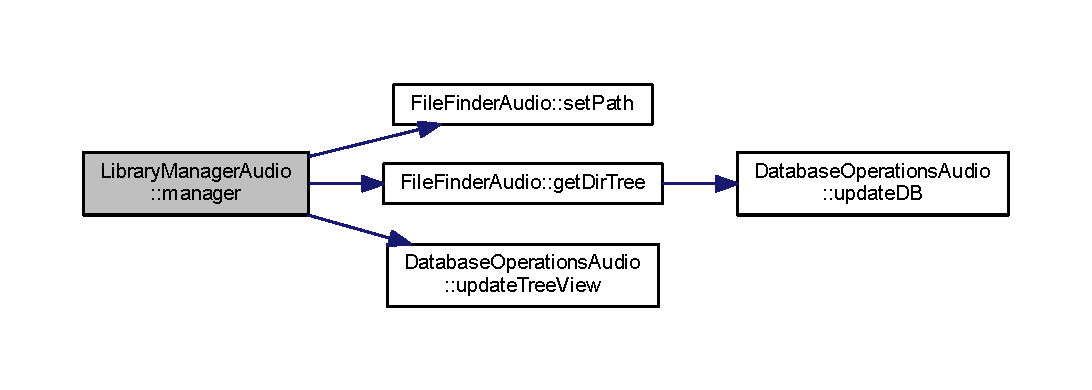
\includegraphics[width=350pt]{class_library_manager_audio_ad2176013457295b02726edb2e6a547c4_cgraph}
\end{center}
\end{figure}


\hypertarget{class_library_manager_audio_a5c1d68b8e484b208dbf43aaf97807e69}{\index{Library\-Manager\-Audio@{Library\-Manager\-Audio}!set\-Destroyer\-Path@{set\-Destroyer\-Path}}
\index{set\-Destroyer\-Path@{set\-Destroyer\-Path}!LibraryManagerAudio@{Library\-Manager\-Audio}}
\subsubsection[{set\-Destroyer\-Path}]{\setlength{\rightskip}{0pt plus 5cm}void Library\-Manager\-Audio\-::set\-Destroyer\-Path (
\begin{DoxyParamCaption}
\item[{Q\-String}]{v\-Path}
\end{DoxyParamCaption}
)}}\label{class_library_manager_audio_a5c1d68b8e484b208dbf43aaf97807e69}


Definition at line 14 of file librarymanageraudio.\-cpp.

\hypertarget{class_library_manager_audio_a3f71d69d66a6b666e02171349950ee8a}{\index{Library\-Manager\-Audio@{Library\-Manager\-Audio}!set\-Initiator\-Path@{set\-Initiator\-Path}}
\index{set\-Initiator\-Path@{set\-Initiator\-Path}!LibraryManagerAudio@{Library\-Manager\-Audio}}
\subsubsection[{set\-Initiator\-Path}]{\setlength{\rightskip}{0pt plus 5cm}void Library\-Manager\-Audio\-::set\-Initiator\-Path (
\begin{DoxyParamCaption}
\item[{Q\-String}]{v\-Path}
\end{DoxyParamCaption}
)}}\label{class_library_manager_audio_a3f71d69d66a6b666e02171349950ee8a}


Definition at line 8 of file librarymanageraudio.\-cpp.



Here is the call graph for this function\-:
\nopagebreak
\begin{figure}[H]
\begin{center}
\leavevmode
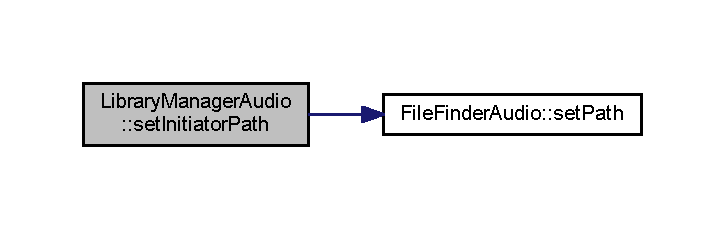
\includegraphics[width=348pt]{class_library_manager_audio_a3f71d69d66a6b666e02171349950ee8a_cgraph}
\end{center}
\end{figure}


\hypertarget{class_library_manager_audio_aeeb16a8820789dcd1680331707c7c72e}{\index{Library\-Manager\-Audio@{Library\-Manager\-Audio}!set\-Manager\-Online@{set\-Manager\-Online}}
\index{set\-Manager\-Online@{set\-Manager\-Online}!LibraryManagerAudio@{Library\-Manager\-Audio}}
\subsubsection[{set\-Manager\-Online}]{\setlength{\rightskip}{0pt plus 5cm}void Library\-Manager\-Audio\-::set\-Manager\-Online (
\begin{DoxyParamCaption}
{}
\end{DoxyParamCaption}
)}}\label{class_library_manager_audio_aeeb16a8820789dcd1680331707c7c72e}


Definition at line 46 of file librarymanageraudio.\-cpp.



The documentation for this class was generated from the following files\-:\begin{DoxyCompactItemize}
\item 
C\-:/\-Users/\-X/\-Documents/\-Qt/\-Media\-Take/\hyperlink{librarymanageraudio_8h}{librarymanageraudio.\-h}\item 
C\-:/\-Users/\-X/\-Documents/\-Qt/\-Media\-Take/\hyperlink{librarymanageraudio_8cpp}{librarymanageraudio.\-cpp}\end{DoxyCompactItemize}

\hypertarget{class_library_manager_video}{\section{Library\-Manager\-Video Class Reference}
\label{class_library_manager_video}\index{Library\-Manager\-Video@{Library\-Manager\-Video}}
}


{\ttfamily \#include $<$librarymanagervideo.\-h$>$}



Inheritance diagram for Library\-Manager\-Video\-:
\nopagebreak
\begin{figure}[H]
\begin{center}
\leavevmode
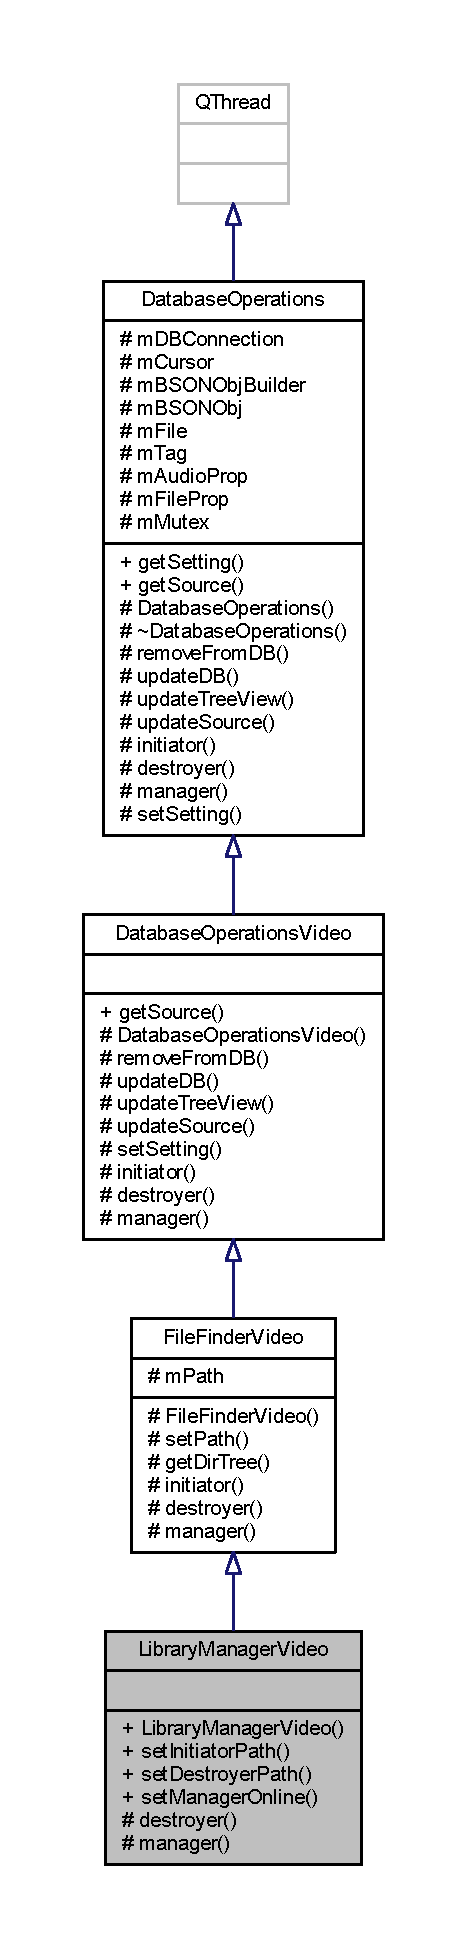
\includegraphics[height=550pt]{class_library_manager_video__inherit__graph}
\end{center}
\end{figure}


Collaboration diagram for Library\-Manager\-Video\-:
\nopagebreak
\begin{figure}[H]
\begin{center}
\leavevmode
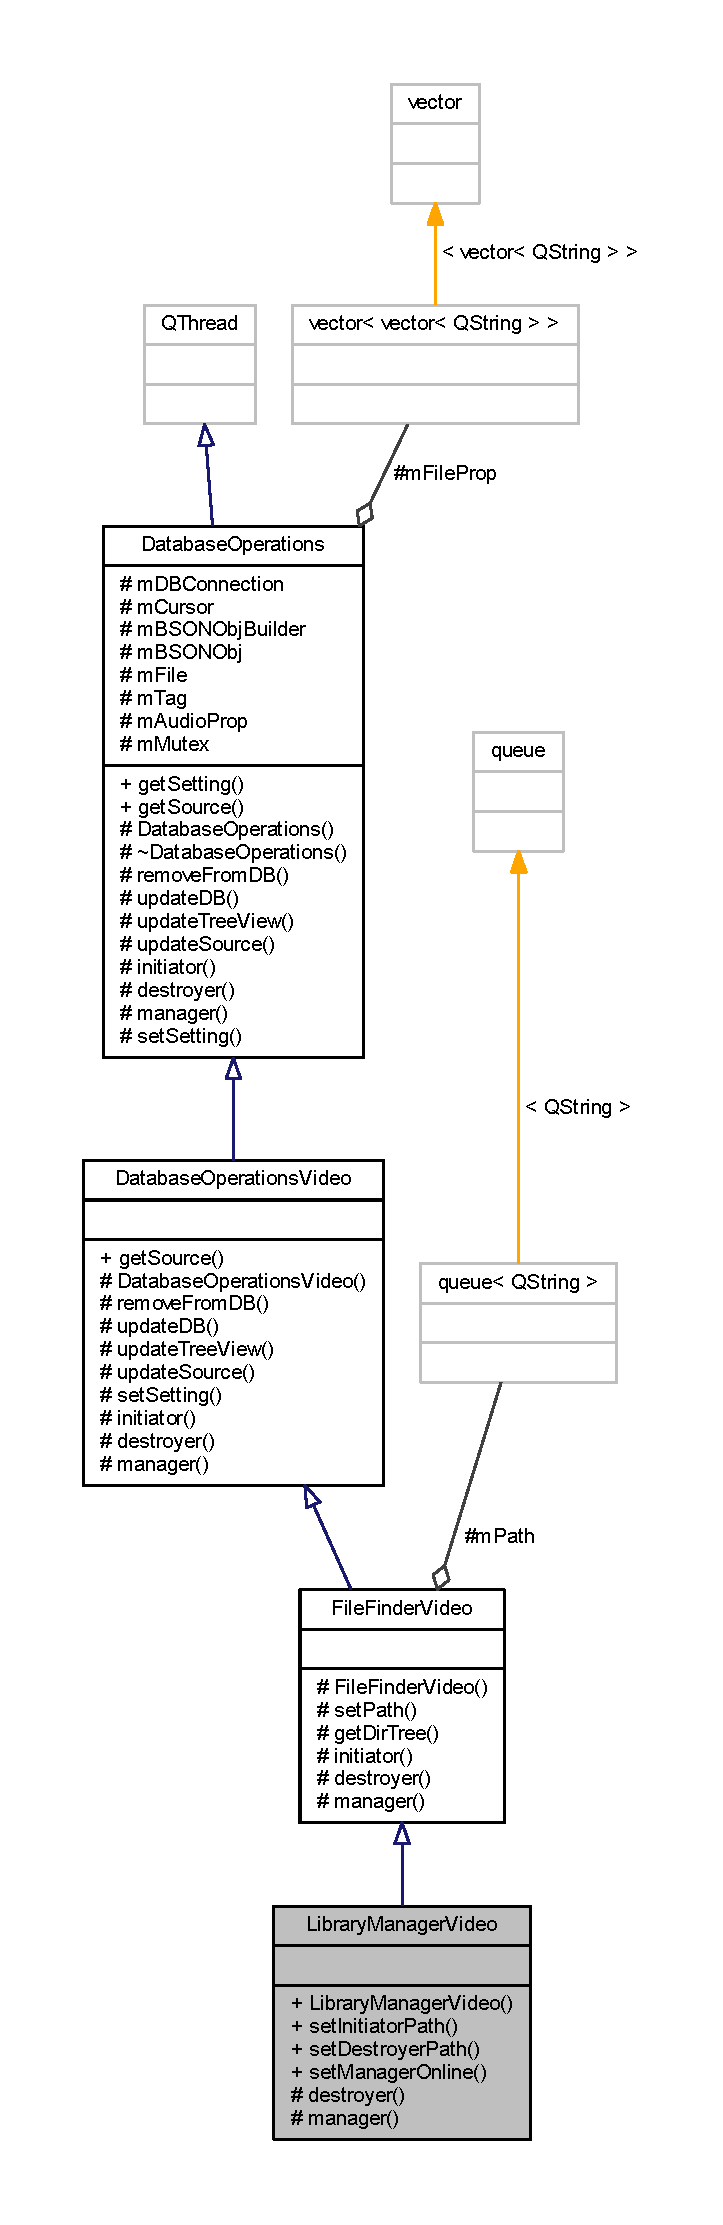
\includegraphics[height=550pt]{class_library_manager_video__coll__graph}
\end{center}
\end{figure}
\subsection*{Public Member Functions}
\begin{DoxyCompactItemize}
\item 
\hyperlink{class_library_manager_video_aaa8e91329f88803b80f2a723954b1188}{Library\-Manager\-Video} (Q\-Object $\ast$parent=0)
\item 
void \hyperlink{class_library_manager_video_a8c448f4da0f3e7b1a821086c45597849}{set\-Initiator\-Path} (Q\-String)
\item 
void \hyperlink{class_library_manager_video_a0a3a3f2221264821f29c4a028dac3334}{set\-Destroyer\-Path} (Q\-String)
\item 
void \hyperlink{class_library_manager_video_ae1883a1f0fa0d98781678e6da2c38f63}{set\-Manager\-Online} ()
\end{DoxyCompactItemize}
\subsection*{Protected Member Functions}
\begin{DoxyCompactItemize}
\item 
void \hyperlink{class_library_manager_video_abdecc35f2d907679a08f32ef8749b9bc}{destroyer} ()
\item 
void \hyperlink{class_library_manager_video_a414263df76f62ab14a3372ba983cd348}{manager} ()
\end{DoxyCompactItemize}
\subsection*{Additional Inherited Members}


\subsection{Detailed Description}


Definition at line 10 of file librarymanagervideo.\-h.



\subsection{Constructor \& Destructor Documentation}
\hypertarget{class_library_manager_video_aaa8e91329f88803b80f2a723954b1188}{\index{Library\-Manager\-Video@{Library\-Manager\-Video}!Library\-Manager\-Video@{Library\-Manager\-Video}}
\index{Library\-Manager\-Video@{Library\-Manager\-Video}!LibraryManagerVideo@{Library\-Manager\-Video}}
\subsubsection[{Library\-Manager\-Video}]{\setlength{\rightskip}{0pt plus 5cm}Library\-Manager\-Video\-::\-Library\-Manager\-Video (
\begin{DoxyParamCaption}
\item[{Q\-Object $\ast$}]{parent = {\ttfamily 0}}
\end{DoxyParamCaption}
)\hspace{0.3cm}{\ttfamily [explicit]}}}\label{class_library_manager_video_aaa8e91329f88803b80f2a723954b1188}


Definition at line 3 of file librarymanagervideo.\-cpp.



\subsection{Member Function Documentation}
\hypertarget{class_library_manager_video_abdecc35f2d907679a08f32ef8749b9bc}{\index{Library\-Manager\-Video@{Library\-Manager\-Video}!destroyer@{destroyer}}
\index{destroyer@{destroyer}!LibraryManagerVideo@{Library\-Manager\-Video}}
\subsubsection[{destroyer}]{\setlength{\rightskip}{0pt plus 5cm}void Library\-Manager\-Video\-::destroyer (
\begin{DoxyParamCaption}
{}
\end{DoxyParamCaption}
)\hspace{0.3cm}{\ttfamily [protected]}, {\ttfamily [virtual]}}}\label{class_library_manager_video_abdecc35f2d907679a08f32ef8749b9bc}


Implements \hyperlink{class_file_finder_video_a37f0b885d2e98d3ac8b6f845c874c63d}{File\-Finder\-Video}.



Definition at line 39 of file librarymanagervideo.\-cpp.



Here is the call graph for this function\-:
\nopagebreak
\begin{figure}[H]
\begin{center}
\leavevmode
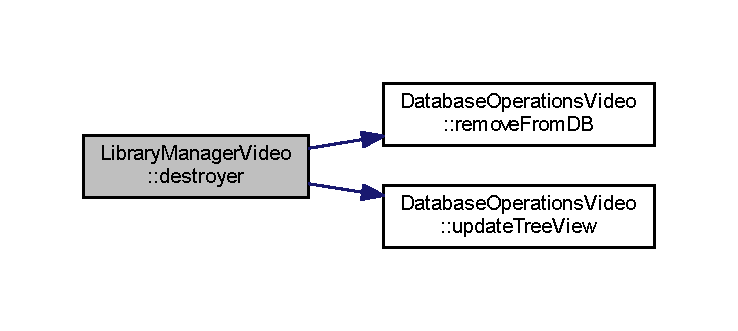
\includegraphics[width=350pt]{class_library_manager_video_abdecc35f2d907679a08f32ef8749b9bc_cgraph}
\end{center}
\end{figure}


\hypertarget{class_library_manager_video_a414263df76f62ab14a3372ba983cd348}{\index{Library\-Manager\-Video@{Library\-Manager\-Video}!manager@{manager}}
\index{manager@{manager}!LibraryManagerVideo@{Library\-Manager\-Video}}
\subsubsection[{manager}]{\setlength{\rightskip}{0pt plus 5cm}void Library\-Manager\-Video\-::manager (
\begin{DoxyParamCaption}
{}
\end{DoxyParamCaption}
)\hspace{0.3cm}{\ttfamily [protected]}, {\ttfamily [virtual]}}}\label{class_library_manager_video_a414263df76f62ab14a3372ba983cd348}


Implements \hyperlink{class_file_finder_video_aafe5126b440c0c5564a32a54fee0781c}{File\-Finder\-Video}.



Definition at line 51 of file librarymanagervideo.\-cpp.



Here is the call graph for this function\-:
\nopagebreak
\begin{figure}[H]
\begin{center}
\leavevmode
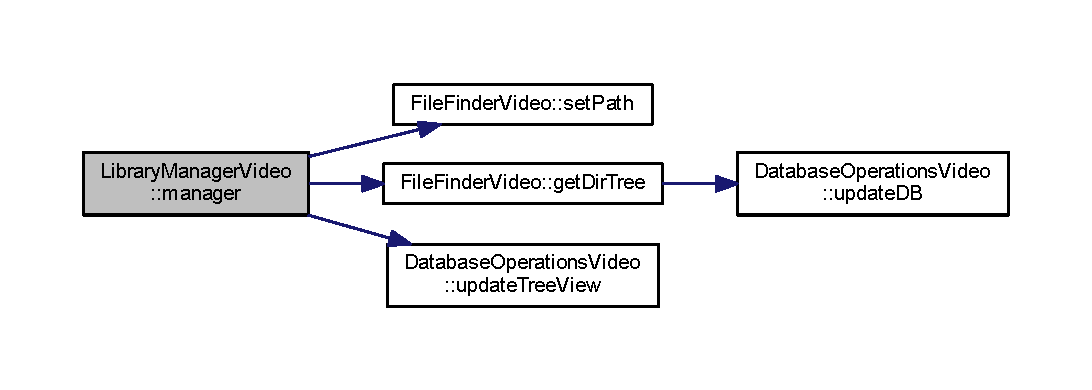
\includegraphics[width=350pt]{class_library_manager_video_a414263df76f62ab14a3372ba983cd348_cgraph}
\end{center}
\end{figure}


\hypertarget{class_library_manager_video_a0a3a3f2221264821f29c4a028dac3334}{\index{Library\-Manager\-Video@{Library\-Manager\-Video}!set\-Destroyer\-Path@{set\-Destroyer\-Path}}
\index{set\-Destroyer\-Path@{set\-Destroyer\-Path}!LibraryManagerVideo@{Library\-Manager\-Video}}
\subsubsection[{set\-Destroyer\-Path}]{\setlength{\rightskip}{0pt plus 5cm}void Library\-Manager\-Video\-::set\-Destroyer\-Path (
\begin{DoxyParamCaption}
\item[{Q\-String}]{v\-Path}
\end{DoxyParamCaption}
)}}\label{class_library_manager_video_a0a3a3f2221264821f29c4a028dac3334}


Definition at line 14 of file librarymanagervideo.\-cpp.

\hypertarget{class_library_manager_video_a8c448f4da0f3e7b1a821086c45597849}{\index{Library\-Manager\-Video@{Library\-Manager\-Video}!set\-Initiator\-Path@{set\-Initiator\-Path}}
\index{set\-Initiator\-Path@{set\-Initiator\-Path}!LibraryManagerVideo@{Library\-Manager\-Video}}
\subsubsection[{set\-Initiator\-Path}]{\setlength{\rightskip}{0pt plus 5cm}void Library\-Manager\-Video\-::set\-Initiator\-Path (
\begin{DoxyParamCaption}
\item[{Q\-String}]{v\-Path}
\end{DoxyParamCaption}
)}}\label{class_library_manager_video_a8c448f4da0f3e7b1a821086c45597849}


Definition at line 8 of file librarymanagervideo.\-cpp.



Here is the call graph for this function\-:
\nopagebreak
\begin{figure}[H]
\begin{center}
\leavevmode
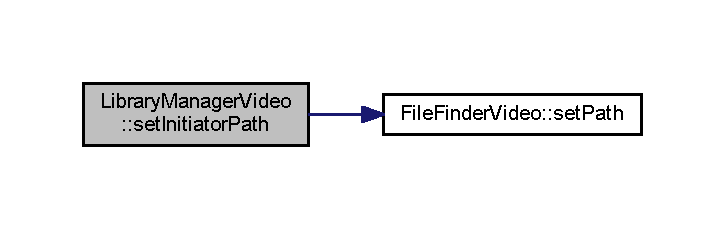
\includegraphics[width=348pt]{class_library_manager_video_a8c448f4da0f3e7b1a821086c45597849_cgraph}
\end{center}
\end{figure}


\hypertarget{class_library_manager_video_ae1883a1f0fa0d98781678e6da2c38f63}{\index{Library\-Manager\-Video@{Library\-Manager\-Video}!set\-Manager\-Online@{set\-Manager\-Online}}
\index{set\-Manager\-Online@{set\-Manager\-Online}!LibraryManagerVideo@{Library\-Manager\-Video}}
\subsubsection[{set\-Manager\-Online}]{\setlength{\rightskip}{0pt plus 5cm}void Library\-Manager\-Video\-::set\-Manager\-Online (
\begin{DoxyParamCaption}
{}
\end{DoxyParamCaption}
)}}\label{class_library_manager_video_ae1883a1f0fa0d98781678e6da2c38f63}


Definition at line 46 of file librarymanagervideo.\-cpp.



The documentation for this class was generated from the following files\-:\begin{DoxyCompactItemize}
\item 
C\-:/\-Users/\-X/\-Documents/\-Qt/\-Media\-Take/\hyperlink{librarymanagervideo_8h}{librarymanagervideo.\-h}\item 
C\-:/\-Users/\-X/\-Documents/\-Qt/\-Media\-Take/\hyperlink{librarymanagervideo_8cpp}{librarymanagervideo.\-cpp}\end{DoxyCompactItemize}

\hypertarget{class_main_window}{\section{Main\-Window Class Reference}
\label{class_main_window}\index{Main\-Window@{Main\-Window}}
}


{\ttfamily \#include $<$mainwindow.\-h$>$}



Inheritance diagram for Main\-Window\-:
\nopagebreak
\begin{figure}[H]
\begin{center}
\leavevmode
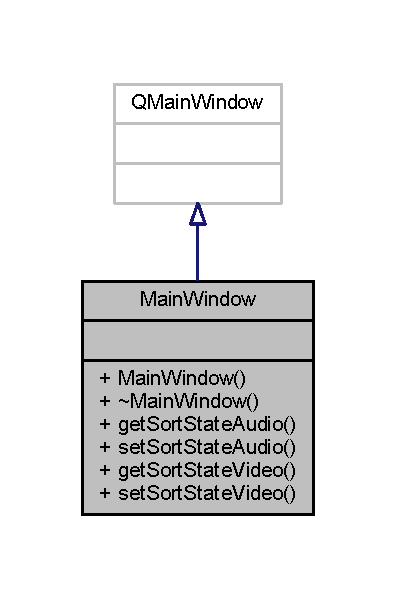
\includegraphics[width=190pt]{class_main_window__inherit__graph}
\end{center}
\end{figure}


Collaboration diagram for Main\-Window\-:
\nopagebreak
\begin{figure}[H]
\begin{center}
\leavevmode
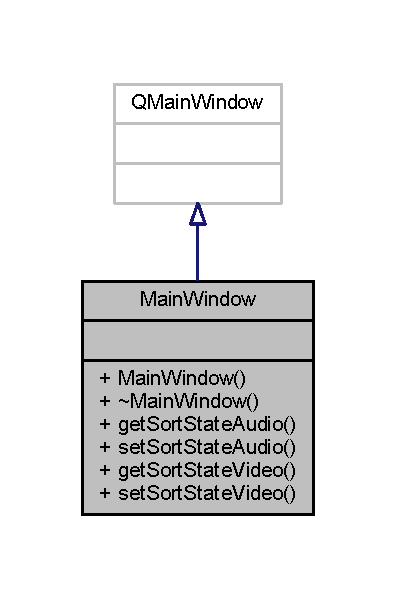
\includegraphics[width=190pt]{class_main_window__coll__graph}
\end{center}
\end{figure}
\subsection*{Signals}
\begin{DoxyCompactItemize}
\item 
void \hyperlink{class_main_window_a9306b3de57fd2e4f6135e2ccb54bb7e8}{set\-Play\-State} ()
\item 
void \hyperlink{class_main_window_adca025abe664d30b94956428bf7018ed}{set\-Pause\-State} ()
\item 
void \hyperlink{class_main_window_ab9186092f55d31ceea72b3033179b3b5}{set\-Stop\-State} ()
\item 
void \hyperlink{class_main_window_a159654f7756ae9e44dfb0d9b9108f5a4}{set\-Video\-Widget\-To\-Audio} (bool)
\item 
void \hyperlink{class_main_window_a52c015261a65b80b1c4bf91a4636eabe}{go\-Full\-Screen} ()
\item 
void \hyperlink{class_main_window_aefcd44e040267b357d7940d01d4b6f82}{set\-Volume\-At\-Video} (int)
\item 
void \hyperlink{class_main_window_a95d2e2f769be6afbe13ca026d22b1936}{set\-Now\-Playing\-Video} (Q\-String)
\end{DoxyCompactItemize}
\subsection*{Public Member Functions}
\begin{DoxyCompactItemize}
\item 
\hyperlink{class_main_window_a8b244be8b7b7db1b08de2a2acb9409db}{Main\-Window} (Q\-Widget $\ast$parent=0)
\item 
\hyperlink{class_main_window_ae98d00a93bc118200eeef9f9bba1dba7}{$\sim$\-Main\-Window} ()
\item 
int \hyperlink{class_main_window_aa5c41c7fa4a061a6f12868c7a45540f2}{get\-Sort\-State\-Audio} ()
\item 
void \hyperlink{class_main_window_af28d26cf9634987d5ed5811c9046227e}{set\-Sort\-State\-Audio} (tree\-Widget\-Sort\-States\-Audio v\-State)
\item 
int \hyperlink{class_main_window_aaba702cedaf6cc6c924cda87607f9504}{get\-Sort\-State\-Video} ()
\item 
void \hyperlink{class_main_window_a85cb80e484e5fb77e1373d005de34c8b}{set\-Sort\-State\-Video} (tree\-Widget\-Sort\-States\-Video v\-State)
\end{DoxyCompactItemize}


\subsection{Detailed Description}


Definition at line 22 of file mainwindow.\-h.



\subsection{Constructor \& Destructor Documentation}
\hypertarget{class_main_window_a8b244be8b7b7db1b08de2a2acb9409db}{\index{Main\-Window@{Main\-Window}!Main\-Window@{Main\-Window}}
\index{Main\-Window@{Main\-Window}!MainWindow@{Main\-Window}}
\subsubsection[{Main\-Window}]{\setlength{\rightskip}{0pt plus 5cm}Main\-Window\-::\-Main\-Window (
\begin{DoxyParamCaption}
\item[{Q\-Widget $\ast$}]{parent = {\ttfamily 0}}
\end{DoxyParamCaption}
)\hspace{0.3cm}{\ttfamily [explicit]}}}\label{class_main_window_a8b244be8b7b7db1b08de2a2acb9409db}


Definition at line 5 of file mainwindow.\-cpp.



Here is the call graph for this function\-:
\nopagebreak
\begin{figure}[H]
\begin{center}
\leavevmode
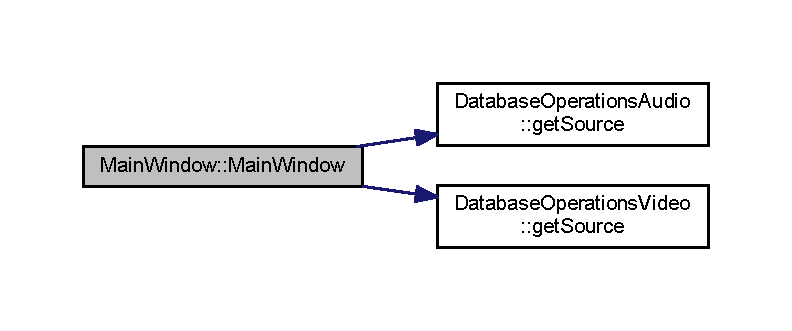
\includegraphics[width=350pt]{class_main_window_a8b244be8b7b7db1b08de2a2acb9409db_cgraph}
\end{center}
\end{figure}


\hypertarget{class_main_window_ae98d00a93bc118200eeef9f9bba1dba7}{\index{Main\-Window@{Main\-Window}!$\sim$\-Main\-Window@{$\sim$\-Main\-Window}}
\index{$\sim$\-Main\-Window@{$\sim$\-Main\-Window}!MainWindow@{Main\-Window}}
\subsubsection[{$\sim$\-Main\-Window}]{\setlength{\rightskip}{0pt plus 5cm}Main\-Window\-::$\sim$\-Main\-Window (
\begin{DoxyParamCaption}
{}
\end{DoxyParamCaption}
)}}\label{class_main_window_ae98d00a93bc118200eeef9f9bba1dba7}


Definition at line 121 of file mainwindow.\-cpp.



\subsection{Member Function Documentation}
\hypertarget{class_main_window_aa5c41c7fa4a061a6f12868c7a45540f2}{\index{Main\-Window@{Main\-Window}!get\-Sort\-State\-Audio@{get\-Sort\-State\-Audio}}
\index{get\-Sort\-State\-Audio@{get\-Sort\-State\-Audio}!MainWindow@{Main\-Window}}
\subsubsection[{get\-Sort\-State\-Audio}]{\setlength{\rightskip}{0pt plus 5cm}int Main\-Window\-::get\-Sort\-State\-Audio (
\begin{DoxyParamCaption}
{}
\end{DoxyParamCaption}
)}}\label{class_main_window_aa5c41c7fa4a061a6f12868c7a45540f2}


Definition at line 433 of file mainwindow.\-cpp.

\hypertarget{class_main_window_aaba702cedaf6cc6c924cda87607f9504}{\index{Main\-Window@{Main\-Window}!get\-Sort\-State\-Video@{get\-Sort\-State\-Video}}
\index{get\-Sort\-State\-Video@{get\-Sort\-State\-Video}!MainWindow@{Main\-Window}}
\subsubsection[{get\-Sort\-State\-Video}]{\setlength{\rightskip}{0pt plus 5cm}int Main\-Window\-::get\-Sort\-State\-Video (
\begin{DoxyParamCaption}
{}
\end{DoxyParamCaption}
)}}\label{class_main_window_aaba702cedaf6cc6c924cda87607f9504}
\hypertarget{class_main_window_a52c015261a65b80b1c4bf91a4636eabe}{\index{Main\-Window@{Main\-Window}!go\-Full\-Screen@{go\-Full\-Screen}}
\index{go\-Full\-Screen@{go\-Full\-Screen}!MainWindow@{Main\-Window}}
\subsubsection[{go\-Full\-Screen}]{\setlength{\rightskip}{0pt plus 5cm}void Main\-Window\-::go\-Full\-Screen (
\begin{DoxyParamCaption}
{}
\end{DoxyParamCaption}
)\hspace{0.3cm}{\ttfamily [signal]}}}\label{class_main_window_a52c015261a65b80b1c4bf91a4636eabe}


Here is the caller graph for this function\-:
\nopagebreak
\begin{figure}[H]
\begin{center}
\leavevmode
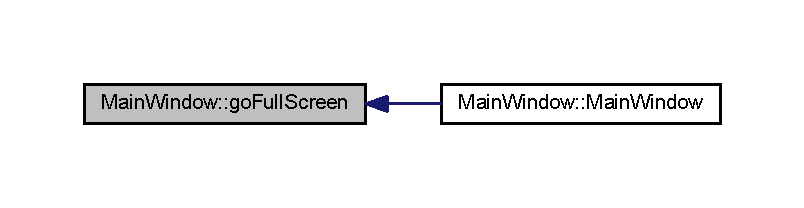
\includegraphics[width=350pt]{class_main_window_a52c015261a65b80b1c4bf91a4636eabe_icgraph}
\end{center}
\end{figure}


\hypertarget{class_main_window_a95d2e2f769be6afbe13ca026d22b1936}{\index{Main\-Window@{Main\-Window}!set\-Now\-Playing\-Video@{set\-Now\-Playing\-Video}}
\index{set\-Now\-Playing\-Video@{set\-Now\-Playing\-Video}!MainWindow@{Main\-Window}}
\subsubsection[{set\-Now\-Playing\-Video}]{\setlength{\rightskip}{0pt plus 5cm}void Main\-Window\-::set\-Now\-Playing\-Video (
\begin{DoxyParamCaption}
\item[{Q\-String}]{}
\end{DoxyParamCaption}
)\hspace{0.3cm}{\ttfamily [signal]}}}\label{class_main_window_a95d2e2f769be6afbe13ca026d22b1936}


Here is the caller graph for this function\-:
\nopagebreak
\begin{figure}[H]
\begin{center}
\leavevmode
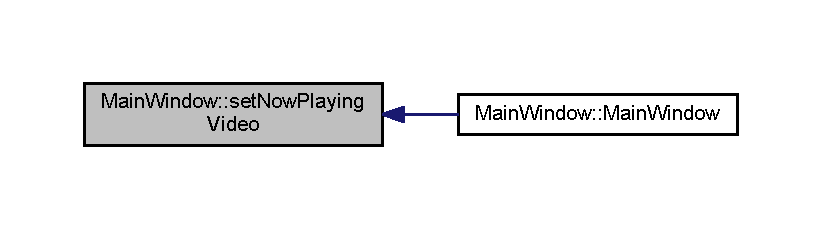
\includegraphics[width=350pt]{class_main_window_a95d2e2f769be6afbe13ca026d22b1936_icgraph}
\end{center}
\end{figure}


\hypertarget{class_main_window_adca025abe664d30b94956428bf7018ed}{\index{Main\-Window@{Main\-Window}!set\-Pause\-State@{set\-Pause\-State}}
\index{set\-Pause\-State@{set\-Pause\-State}!MainWindow@{Main\-Window}}
\subsubsection[{set\-Pause\-State}]{\setlength{\rightskip}{0pt plus 5cm}void Main\-Window\-::set\-Pause\-State (
\begin{DoxyParamCaption}
{}
\end{DoxyParamCaption}
)\hspace{0.3cm}{\ttfamily [signal]}}}\label{class_main_window_adca025abe664d30b94956428bf7018ed}


Here is the caller graph for this function\-:
\nopagebreak
\begin{figure}[H]
\begin{center}
\leavevmode
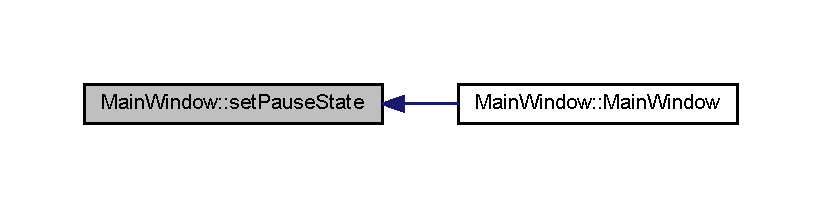
\includegraphics[width=350pt]{class_main_window_adca025abe664d30b94956428bf7018ed_icgraph}
\end{center}
\end{figure}


\hypertarget{class_main_window_a9306b3de57fd2e4f6135e2ccb54bb7e8}{\index{Main\-Window@{Main\-Window}!set\-Play\-State@{set\-Play\-State}}
\index{set\-Play\-State@{set\-Play\-State}!MainWindow@{Main\-Window}}
\subsubsection[{set\-Play\-State}]{\setlength{\rightskip}{0pt plus 5cm}void Main\-Window\-::set\-Play\-State (
\begin{DoxyParamCaption}
{}
\end{DoxyParamCaption}
)\hspace{0.3cm}{\ttfamily [signal]}}}\label{class_main_window_a9306b3de57fd2e4f6135e2ccb54bb7e8}


Here is the caller graph for this function\-:
\nopagebreak
\begin{figure}[H]
\begin{center}
\leavevmode
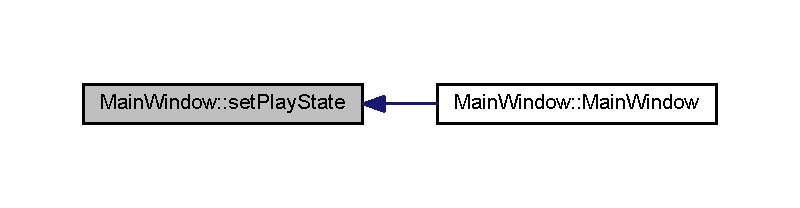
\includegraphics[width=350pt]{class_main_window_a9306b3de57fd2e4f6135e2ccb54bb7e8_icgraph}
\end{center}
\end{figure}


\hypertarget{class_main_window_af28d26cf9634987d5ed5811c9046227e}{\index{Main\-Window@{Main\-Window}!set\-Sort\-State\-Audio@{set\-Sort\-State\-Audio}}
\index{set\-Sort\-State\-Audio@{set\-Sort\-State\-Audio}!MainWindow@{Main\-Window}}
\subsubsection[{set\-Sort\-State\-Audio}]{\setlength{\rightskip}{0pt plus 5cm}void Main\-Window\-::set\-Sort\-State\-Audio (
\begin{DoxyParamCaption}
\item[{tree\-Widget\-Sort\-States\-Audio}]{v\-State}
\end{DoxyParamCaption}
)}}\label{class_main_window_af28d26cf9634987d5ed5811c9046227e}


Definition at line 440 of file mainwindow.\-cpp.

\hypertarget{class_main_window_a85cb80e484e5fb77e1373d005de34c8b}{\index{Main\-Window@{Main\-Window}!set\-Sort\-State\-Video@{set\-Sort\-State\-Video}}
\index{set\-Sort\-State\-Video@{set\-Sort\-State\-Video}!MainWindow@{Main\-Window}}
\subsubsection[{set\-Sort\-State\-Video}]{\setlength{\rightskip}{0pt plus 5cm}void Main\-Window\-::set\-Sort\-State\-Video (
\begin{DoxyParamCaption}
\item[{tree\-Widget\-Sort\-States\-Video}]{v\-State}
\end{DoxyParamCaption}
)}}\label{class_main_window_a85cb80e484e5fb77e1373d005de34c8b}
\hypertarget{class_main_window_ab9186092f55d31ceea72b3033179b3b5}{\index{Main\-Window@{Main\-Window}!set\-Stop\-State@{set\-Stop\-State}}
\index{set\-Stop\-State@{set\-Stop\-State}!MainWindow@{Main\-Window}}
\subsubsection[{set\-Stop\-State}]{\setlength{\rightskip}{0pt plus 5cm}void Main\-Window\-::set\-Stop\-State (
\begin{DoxyParamCaption}
{}
\end{DoxyParamCaption}
)\hspace{0.3cm}{\ttfamily [signal]}}}\label{class_main_window_ab9186092f55d31ceea72b3033179b3b5}


Here is the caller graph for this function\-:
\nopagebreak
\begin{figure}[H]
\begin{center}
\leavevmode
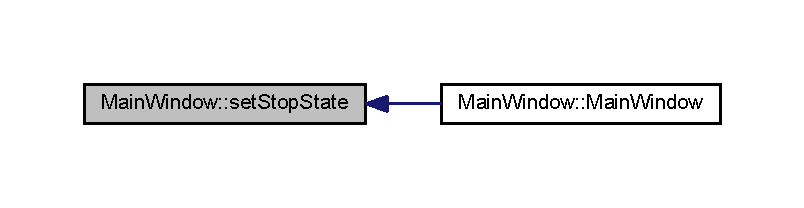
\includegraphics[width=350pt]{class_main_window_ab9186092f55d31ceea72b3033179b3b5_icgraph}
\end{center}
\end{figure}


\hypertarget{class_main_window_a159654f7756ae9e44dfb0d9b9108f5a4}{\index{Main\-Window@{Main\-Window}!set\-Video\-Widget\-To\-Audio@{set\-Video\-Widget\-To\-Audio}}
\index{set\-Video\-Widget\-To\-Audio@{set\-Video\-Widget\-To\-Audio}!MainWindow@{Main\-Window}}
\subsubsection[{set\-Video\-Widget\-To\-Audio}]{\setlength{\rightskip}{0pt plus 5cm}void Main\-Window\-::set\-Video\-Widget\-To\-Audio (
\begin{DoxyParamCaption}
\item[{bool}]{}
\end{DoxyParamCaption}
)\hspace{0.3cm}{\ttfamily [signal]}}}\label{class_main_window_a159654f7756ae9e44dfb0d9b9108f5a4}
\hypertarget{class_main_window_aefcd44e040267b357d7940d01d4b6f82}{\index{Main\-Window@{Main\-Window}!set\-Volume\-At\-Video@{set\-Volume\-At\-Video}}
\index{set\-Volume\-At\-Video@{set\-Volume\-At\-Video}!MainWindow@{Main\-Window}}
\subsubsection[{set\-Volume\-At\-Video}]{\setlength{\rightskip}{0pt plus 5cm}void Main\-Window\-::set\-Volume\-At\-Video (
\begin{DoxyParamCaption}
\item[{int}]{}
\end{DoxyParamCaption}
)\hspace{0.3cm}{\ttfamily [signal]}}}\label{class_main_window_aefcd44e040267b357d7940d01d4b6f82}


Here is the caller graph for this function\-:
\nopagebreak
\begin{figure}[H]
\begin{center}
\leavevmode
\includegraphics[width=350pt]{class_main_window_aefcd44e040267b357d7940d01d4b6f82_icgraph}
\end{center}
\end{figure}




The documentation for this class was generated from the following files\-:\begin{DoxyCompactItemize}
\item 
C\-:/\-Users/\-X/\-Documents/\-Qt/\-Media\-Take/\hyperlink{mainwindow_8h}{mainwindow.\-h}\item 
C\-:/\-Users/\-X/\-Documents/\-Qt/\-Media\-Take/\hyperlink{mainwindow_8cpp}{mainwindow.\-cpp}\end{DoxyCompactItemize}

\hypertarget{class_qt_g_streamer_driver}{\section{Qt\-G\-Streamer\-Driver Class Reference}
\label{class_qt_g_streamer_driver}\index{Qt\-G\-Streamer\-Driver@{Qt\-G\-Streamer\-Driver}}
}


{\ttfamily \#include $<$qtgstreamerdriver.\-h$>$}



Inheritance diagram for Qt\-G\-Streamer\-Driver\-:
\nopagebreak
\begin{figure}[H]
\begin{center}
\leavevmode
\includegraphics[width=198pt]{class_qt_g_streamer_driver__inherit__graph}
\end{center}
\end{figure}


Collaboration diagram for Qt\-G\-Streamer\-Driver\-:
\nopagebreak
\begin{figure}[H]
\begin{center}
\leavevmode
\includegraphics[width=198pt]{class_qt_g_streamer_driver__coll__graph}
\end{center}
\end{figure}
\subsection*{Public Slots}
\begin{DoxyCompactItemize}
\item 
void \hyperlink{class_qt_g_streamer_driver_a1da349939a8952bef19caa3dc1398793}{play} ()
\item 
void \hyperlink{class_qt_g_streamer_driver_a989eef1d9bf2d0686d1c46240b159197}{pause} ()
\item 
void \hyperlink{class_qt_g_streamer_driver_afdc955e0b961bc7731bc0018ac147107}{stop} ()
\item 
void \hyperlink{class_qt_g_streamer_driver_a9a12e01f670bb3df69e5fc7547365be7}{set\-Volume} (int volume)
\end{DoxyCompactItemize}
\subsection*{Signals}
\begin{DoxyCompactItemize}
\item 
void \hyperlink{class_qt_g_streamer_driver_a923a5a22f33296d53115ad54b9ed80e6}{position\-Changed} ()
\item 
void \hyperlink{class_qt_g_streamer_driver_ae6739c0a756de50aa2e2b5a6984fb378}{state\-Changed} ()
\end{DoxyCompactItemize}
\subsection*{Public Member Functions}
\begin{DoxyCompactItemize}
\item 
\hyperlink{class_qt_g_streamer_driver_a80a93e166dac396a210e3cc37b08409a}{Qt\-G\-Streamer\-Driver} (Q\-Widget $\ast$parent=0)
\item 
\hyperlink{class_qt_g_streamer_driver_a02a513ffb6bdeda4329826b3f39d0ebf}{$\sim$\-Qt\-G\-Streamer\-Driver} ()
\item 
int \hyperlink{class_qt_g_streamer_driver_af0a07904dc3a585850357b0630b3c3cf}{get\-Volume} ()
\item 
Q\-Time \hyperlink{class_qt_g_streamer_driver_affb50dcbbfc2033af59b5e6b16a8bada}{get\-Position} ()
\item 
Q\-Time \hyperlink{class_qt_g_streamer_driver_ade7d6d9cf283749bb39e779a6c5b1a4d}{get\-Duration} ()
\item 
Q\-Gst\-::\-State \hyperlink{class_qt_g_streamer_driver_a4badd176ac10373972d10b45f94a3df3}{get\-State} ()
\item 
void \hyperlink{class_qt_g_streamer_driver_adec3a39ff61493bc0191c27a4e7bf8b7}{set\-Path} (Q\-String)
\item 
void \hyperlink{class_qt_g_streamer_driver_a3bec92239fa7147c03bfcb37eeac305b}{set\-Position} (Q\-Time)
\end{DoxyCompactItemize}


\subsection{Detailed Description}


Definition at line 18 of file qtgstreamerdriver.\-h.



\subsection{Constructor \& Destructor Documentation}
\hypertarget{class_qt_g_streamer_driver_a80a93e166dac396a210e3cc37b08409a}{\index{Qt\-G\-Streamer\-Driver@{Qt\-G\-Streamer\-Driver}!Qt\-G\-Streamer\-Driver@{Qt\-G\-Streamer\-Driver}}
\index{Qt\-G\-Streamer\-Driver@{Qt\-G\-Streamer\-Driver}!QtGStreamerDriver@{Qt\-G\-Streamer\-Driver}}
\subsubsection[{Qt\-G\-Streamer\-Driver}]{\setlength{\rightskip}{0pt plus 5cm}Qt\-G\-Streamer\-Driver\-::\-Qt\-G\-Streamer\-Driver (
\begin{DoxyParamCaption}
\item[{Q\-Widget $\ast$}]{parent = {\ttfamily 0}}
\end{DoxyParamCaption}
)}}\label{class_qt_g_streamer_driver_a80a93e166dac396a210e3cc37b08409a}


Definition at line 3 of file qtgstreamerdriver.\-cpp.



Here is the call graph for this function\-:
\nopagebreak
\begin{figure}[H]
\begin{center}
\leavevmode
\includegraphics[width=324pt]{class_qt_g_streamer_driver_a80a93e166dac396a210e3cc37b08409a_cgraph}
\end{center}
\end{figure}


\hypertarget{class_qt_g_streamer_driver_a02a513ffb6bdeda4329826b3f39d0ebf}{\index{Qt\-G\-Streamer\-Driver@{Qt\-G\-Streamer\-Driver}!$\sim$\-Qt\-G\-Streamer\-Driver@{$\sim$\-Qt\-G\-Streamer\-Driver}}
\index{$\sim$\-Qt\-G\-Streamer\-Driver@{$\sim$\-Qt\-G\-Streamer\-Driver}!QtGStreamerDriver@{Qt\-G\-Streamer\-Driver}}
\subsubsection[{$\sim$\-Qt\-G\-Streamer\-Driver}]{\setlength{\rightskip}{0pt plus 5cm}Qt\-G\-Streamer\-Driver\-::$\sim$\-Qt\-G\-Streamer\-Driver (
\begin{DoxyParamCaption}
{}
\end{DoxyParamCaption}
)}}\label{class_qt_g_streamer_driver_a02a513ffb6bdeda4329826b3f39d0ebf}


Definition at line 9 of file qtgstreamerdriver.\-cpp.



\subsection{Member Function Documentation}
\hypertarget{class_qt_g_streamer_driver_ade7d6d9cf283749bb39e779a6c5b1a4d}{\index{Qt\-G\-Streamer\-Driver@{Qt\-G\-Streamer\-Driver}!get\-Duration@{get\-Duration}}
\index{get\-Duration@{get\-Duration}!QtGStreamerDriver@{Qt\-G\-Streamer\-Driver}}
\subsubsection[{get\-Duration}]{\setlength{\rightskip}{0pt plus 5cm}Q\-Time Qt\-G\-Streamer\-Driver\-::get\-Duration (
\begin{DoxyParamCaption}
{}
\end{DoxyParamCaption}
)}}\label{class_qt_g_streamer_driver_ade7d6d9cf283749bb39e779a6c5b1a4d}


Definition at line 156 of file qtgstreamerdriver.\-cpp.

\hypertarget{class_qt_g_streamer_driver_affb50dcbbfc2033af59b5e6b16a8bada}{\index{Qt\-G\-Streamer\-Driver@{Qt\-G\-Streamer\-Driver}!get\-Position@{get\-Position}}
\index{get\-Position@{get\-Position}!QtGStreamerDriver@{Qt\-G\-Streamer\-Driver}}
\subsubsection[{get\-Position}]{\setlength{\rightskip}{0pt plus 5cm}Q\-Time Qt\-G\-Streamer\-Driver\-::get\-Position (
\begin{DoxyParamCaption}
{}
\end{DoxyParamCaption}
)}}\label{class_qt_g_streamer_driver_affb50dcbbfc2033af59b5e6b16a8bada}


Definition at line 128 of file qtgstreamerdriver.\-cpp.

\hypertarget{class_qt_g_streamer_driver_a4badd176ac10373972d10b45f94a3df3}{\index{Qt\-G\-Streamer\-Driver@{Qt\-G\-Streamer\-Driver}!get\-State@{get\-State}}
\index{get\-State@{get\-State}!QtGStreamerDriver@{Qt\-G\-Streamer\-Driver}}
\subsubsection[{get\-State}]{\setlength{\rightskip}{0pt plus 5cm}Q\-Gst\-::\-State Qt\-G\-Streamer\-Driver\-::get\-State (
\begin{DoxyParamCaption}
{}
\end{DoxyParamCaption}
)}}\label{class_qt_g_streamer_driver_a4badd176ac10373972d10b45f94a3df3}


Definition at line 170 of file qtgstreamerdriver.\-cpp.

\hypertarget{class_qt_g_streamer_driver_af0a07904dc3a585850357b0630b3c3cf}{\index{Qt\-G\-Streamer\-Driver@{Qt\-G\-Streamer\-Driver}!get\-Volume@{get\-Volume}}
\index{get\-Volume@{get\-Volume}!QtGStreamerDriver@{Qt\-G\-Streamer\-Driver}}
\subsubsection[{get\-Volume}]{\setlength{\rightskip}{0pt plus 5cm}int Qt\-G\-Streamer\-Driver\-::get\-Volume (
\begin{DoxyParamCaption}
{}
\end{DoxyParamCaption}
)}}\label{class_qt_g_streamer_driver_af0a07904dc3a585850357b0630b3c3cf}


Definition at line 141 of file qtgstreamerdriver.\-cpp.

\hypertarget{class_qt_g_streamer_driver_a989eef1d9bf2d0686d1c46240b159197}{\index{Qt\-G\-Streamer\-Driver@{Qt\-G\-Streamer\-Driver}!pause@{pause}}
\index{pause@{pause}!QtGStreamerDriver@{Qt\-G\-Streamer\-Driver}}
\subsubsection[{pause}]{\setlength{\rightskip}{0pt plus 5cm}void Qt\-G\-Streamer\-Driver\-::pause (
\begin{DoxyParamCaption}
{}
\end{DoxyParamCaption}
)\hspace{0.3cm}{\ttfamily [slot]}}}\label{class_qt_g_streamer_driver_a989eef1d9bf2d0686d1c46240b159197}


Definition at line 192 of file qtgstreamerdriver.\-cpp.

\hypertarget{class_qt_g_streamer_driver_a1da349939a8952bef19caa3dc1398793}{\index{Qt\-G\-Streamer\-Driver@{Qt\-G\-Streamer\-Driver}!play@{play}}
\index{play@{play}!QtGStreamerDriver@{Qt\-G\-Streamer\-Driver}}
\subsubsection[{play}]{\setlength{\rightskip}{0pt plus 5cm}void Qt\-G\-Streamer\-Driver\-::play (
\begin{DoxyParamCaption}
{}
\end{DoxyParamCaption}
)\hspace{0.3cm}{\ttfamily [slot]}}}\label{class_qt_g_streamer_driver_a1da349939a8952bef19caa3dc1398793}


Definition at line 184 of file qtgstreamerdriver.\-cpp.

\hypertarget{class_qt_g_streamer_driver_a923a5a22f33296d53115ad54b9ed80e6}{\index{Qt\-G\-Streamer\-Driver@{Qt\-G\-Streamer\-Driver}!position\-Changed@{position\-Changed}}
\index{position\-Changed@{position\-Changed}!QtGStreamerDriver@{Qt\-G\-Streamer\-Driver}}
\subsubsection[{position\-Changed}]{\setlength{\rightskip}{0pt plus 5cm}void Qt\-G\-Streamer\-Driver\-::position\-Changed (
\begin{DoxyParamCaption}
{}
\end{DoxyParamCaption}
)\hspace{0.3cm}{\ttfamily [signal]}}}\label{class_qt_g_streamer_driver_a923a5a22f33296d53115ad54b9ed80e6}


Here is the caller graph for this function\-:
\nopagebreak
\begin{figure}[H]
\begin{center}
\leavevmode
\includegraphics[width=324pt]{class_qt_g_streamer_driver_a923a5a22f33296d53115ad54b9ed80e6_icgraph}
\end{center}
\end{figure}


\hypertarget{class_qt_g_streamer_driver_adec3a39ff61493bc0191c27a4e7bf8b7}{\index{Qt\-G\-Streamer\-Driver@{Qt\-G\-Streamer\-Driver}!set\-Path@{set\-Path}}
\index{set\-Path@{set\-Path}!QtGStreamerDriver@{Qt\-G\-Streamer\-Driver}}
\subsubsection[{set\-Path}]{\setlength{\rightskip}{0pt plus 5cm}void Qt\-G\-Streamer\-Driver\-::set\-Path (
\begin{DoxyParamCaption}
\item[{Q\-String}]{v\-Path}
\end{DoxyParamCaption}
)}}\label{class_qt_g_streamer_driver_adec3a39ff61493bc0191c27a4e7bf8b7}


Definition at line 82 of file qtgstreamerdriver.\-cpp.

\hypertarget{class_qt_g_streamer_driver_a3bec92239fa7147c03bfcb37eeac305b}{\index{Qt\-G\-Streamer\-Driver@{Qt\-G\-Streamer\-Driver}!set\-Position@{set\-Position}}
\index{set\-Position@{set\-Position}!QtGStreamerDriver@{Qt\-G\-Streamer\-Driver}}
\subsubsection[{set\-Position}]{\setlength{\rightskip}{0pt plus 5cm}void Qt\-G\-Streamer\-Driver\-::set\-Position (
\begin{DoxyParamCaption}
\item[{Q\-Time}]{v\-Position}
\end{DoxyParamCaption}
)}}\label{class_qt_g_streamer_driver_a3bec92239fa7147c03bfcb37eeac305b}


Definition at line 117 of file qtgstreamerdriver.\-cpp.

\hypertarget{class_qt_g_streamer_driver_a9a12e01f670bb3df69e5fc7547365be7}{\index{Qt\-G\-Streamer\-Driver@{Qt\-G\-Streamer\-Driver}!set\-Volume@{set\-Volume}}
\index{set\-Volume@{set\-Volume}!QtGStreamerDriver@{Qt\-G\-Streamer\-Driver}}
\subsubsection[{set\-Volume}]{\setlength{\rightskip}{0pt plus 5cm}void Qt\-G\-Streamer\-Driver\-::set\-Volume (
\begin{DoxyParamCaption}
\item[{int}]{volume}
\end{DoxyParamCaption}
)\hspace{0.3cm}{\ttfamily [slot]}}}\label{class_qt_g_streamer_driver_a9a12e01f670bb3df69e5fc7547365be7}


Definition at line 213 of file qtgstreamerdriver.\-cpp.



Here is the caller graph for this function\-:
\nopagebreak
\begin{figure}[H]
\begin{center}
\leavevmode
\includegraphics[width=324pt]{class_qt_g_streamer_driver_a9a12e01f670bb3df69e5fc7547365be7_icgraph}
\end{center}
\end{figure}


\hypertarget{class_qt_g_streamer_driver_ae6739c0a756de50aa2e2b5a6984fb378}{\index{Qt\-G\-Streamer\-Driver@{Qt\-G\-Streamer\-Driver}!state\-Changed@{state\-Changed}}
\index{state\-Changed@{state\-Changed}!QtGStreamerDriver@{Qt\-G\-Streamer\-Driver}}
\subsubsection[{state\-Changed}]{\setlength{\rightskip}{0pt plus 5cm}void Qt\-G\-Streamer\-Driver\-::state\-Changed (
\begin{DoxyParamCaption}
{}
\end{DoxyParamCaption}
)\hspace{0.3cm}{\ttfamily [signal]}}}\label{class_qt_g_streamer_driver_ae6739c0a756de50aa2e2b5a6984fb378}


Here is the caller graph for this function\-:
\nopagebreak
\begin{figure}[H]
\begin{center}
\leavevmode
\includegraphics[width=344pt]{class_qt_g_streamer_driver_ae6739c0a756de50aa2e2b5a6984fb378_icgraph}
\end{center}
\end{figure}


\hypertarget{class_qt_g_streamer_driver_afdc955e0b961bc7731bc0018ac147107}{\index{Qt\-G\-Streamer\-Driver@{Qt\-G\-Streamer\-Driver}!stop@{stop}}
\index{stop@{stop}!QtGStreamerDriver@{Qt\-G\-Streamer\-Driver}}
\subsubsection[{stop}]{\setlength{\rightskip}{0pt plus 5cm}void Qt\-G\-Streamer\-Driver\-::stop (
\begin{DoxyParamCaption}
{}
\end{DoxyParamCaption}
)\hspace{0.3cm}{\ttfamily [slot]}}}\label{class_qt_g_streamer_driver_afdc955e0b961bc7731bc0018ac147107}


Definition at line 200 of file qtgstreamerdriver.\-cpp.



The documentation for this class was generated from the following files\-:\begin{DoxyCompactItemize}
\item 
C\-:/\-Users/\-X/\-Documents/\-Qt/\-Media\-Take/\hyperlink{qtgstreamerdriver_8h}{qtgstreamerdriver.\-h}\item 
C\-:/\-Users/\-X/\-Documents/\-Qt/\-Media\-Take/\hyperlink{qtgstreamerdriver_8cpp}{qtgstreamerdriver.\-cpp}\end{DoxyCompactItemize}

\hypertarget{class_select_file_dialog}{\section{Select\-File\-Dialog Class Reference}
\label{class_select_file_dialog}\index{Select\-File\-Dialog@{Select\-File\-Dialog}}
}


{\ttfamily \#include $<$selectfiledialog.\-h$>$}



Inheritance diagram for Select\-File\-Dialog\-:
\nopagebreak
\begin{figure}[H]
\begin{center}
\leavevmode
\includegraphics[width=188pt]{class_select_file_dialog__inherit__graph}
\end{center}
\end{figure}


Collaboration diagram for Select\-File\-Dialog\-:
\nopagebreak
\begin{figure}[H]
\begin{center}
\leavevmode
\includegraphics[width=188pt]{class_select_file_dialog__coll__graph}
\end{center}
\end{figure}
\subsection*{Signals}
\begin{DoxyCompactItemize}
\item 
void \hyperlink{class_select_file_dialog_ab1c1d6c23dd822f6228a98a8981c49bd}{selected\-Path} (Q\-String)
\end{DoxyCompactItemize}
\subsection*{Public Member Functions}
\begin{DoxyCompactItemize}
\item 
\hyperlink{class_select_file_dialog_a5ea045c74c9fd9402dcd4089319eb19d}{Select\-File\-Dialog} (Q\-Widget $\ast$parent=0)
\item 
\hyperlink{class_select_file_dialog_a7cdede4614b15a79d24346ede9db7c00}{$\sim$\-Select\-File\-Dialog} ()
\end{DoxyCompactItemize}


\subsection{Detailed Description}


Definition at line 13 of file selectfiledialog.\-h.



\subsection{Constructor \& Destructor Documentation}
\hypertarget{class_select_file_dialog_a5ea045c74c9fd9402dcd4089319eb19d}{\index{Select\-File\-Dialog@{Select\-File\-Dialog}!Select\-File\-Dialog@{Select\-File\-Dialog}}
\index{Select\-File\-Dialog@{Select\-File\-Dialog}!SelectFileDialog@{Select\-File\-Dialog}}
\subsubsection[{Select\-File\-Dialog}]{\setlength{\rightskip}{0pt plus 5cm}Select\-File\-Dialog\-::\-Select\-File\-Dialog (
\begin{DoxyParamCaption}
\item[{Q\-Widget $\ast$}]{parent = {\ttfamily 0}}
\end{DoxyParamCaption}
)\hspace{0.3cm}{\ttfamily [explicit]}}}\label{class_select_file_dialog_a5ea045c74c9fd9402dcd4089319eb19d}


Definition at line 4 of file selectfiledialog.\-cpp.

\hypertarget{class_select_file_dialog_a7cdede4614b15a79d24346ede9db7c00}{\index{Select\-File\-Dialog@{Select\-File\-Dialog}!$\sim$\-Select\-File\-Dialog@{$\sim$\-Select\-File\-Dialog}}
\index{$\sim$\-Select\-File\-Dialog@{$\sim$\-Select\-File\-Dialog}!SelectFileDialog@{Select\-File\-Dialog}}
\subsubsection[{$\sim$\-Select\-File\-Dialog}]{\setlength{\rightskip}{0pt plus 5cm}Select\-File\-Dialog\-::$\sim$\-Select\-File\-Dialog (
\begin{DoxyParamCaption}
{}
\end{DoxyParamCaption}
)}}\label{class_select_file_dialog_a7cdede4614b15a79d24346ede9db7c00}


Definition at line 26 of file selectfiledialog.\-cpp.



\subsection{Member Function Documentation}
\hypertarget{class_select_file_dialog_ab1c1d6c23dd822f6228a98a8981c49bd}{\index{Select\-File\-Dialog@{Select\-File\-Dialog}!selected\-Path@{selected\-Path}}
\index{selected\-Path@{selected\-Path}!SelectFileDialog@{Select\-File\-Dialog}}
\subsubsection[{selected\-Path}]{\setlength{\rightskip}{0pt plus 5cm}void Select\-File\-Dialog\-::selected\-Path (
\begin{DoxyParamCaption}
\item[{Q\-String}]{}
\end{DoxyParamCaption}
)\hspace{0.3cm}{\ttfamily [signal]}}}\label{class_select_file_dialog_ab1c1d6c23dd822f6228a98a8981c49bd}


The documentation for this class was generated from the following files\-:\begin{DoxyCompactItemize}
\item 
C\-:/\-Users/\-X/\-Documents/\-Qt/\-Media\-Take/\hyperlink{selectfiledialog_8h}{selectfiledialog.\-h}\item 
C\-:/\-Users/\-X/\-Documents/\-Qt/\-Media\-Take/\hyperlink{selectfiledialog_8cpp}{selectfiledialog.\-cpp}\end{DoxyCompactItemize}

\hypertarget{class_video_sink}{\section{Video\-Sink Class Reference}
\label{class_video_sink}\index{Video\-Sink@{Video\-Sink}}
}


{\ttfamily \#include $<$videosink.\-h$>$}



Inheritance diagram for Video\-Sink\-:
\nopagebreak
\begin{figure}[H]
\begin{center}
\leavevmode
\includegraphics[width=162pt]{class_video_sink__inherit__graph}
\end{center}
\end{figure}


Collaboration diagram for Video\-Sink\-:
\nopagebreak
\begin{figure}[H]
\begin{center}
\leavevmode
\includegraphics[width=162pt]{class_video_sink__coll__graph}
\end{center}
\end{figure}
\subsection*{Signals}
\begin{DoxyCompactItemize}
\item 
void \hyperlink{class_video_sink_a11a4d7487a57ee038cc981c68330ff1f}{close\-Main} ()
\item 
void \hyperlink{class_video_sink_af5d1a52c838dc1c73a23c42e08edcdf7}{next\-Clicked} ()
\item 
void \hyperlink{class_video_sink_ab4bccb7758df596104e7f8a7860b5480}{prev\-Clicked} ()
\item 
void \hyperlink{class_video_sink_acf83d2282f84a361b11a34c55e5498c5}{set\-Pause\-State} ()
\item 
void \hyperlink{class_video_sink_ae11b1fd8e421c6aadee7874bbbd4ff3d}{set\-Play\-State} ()
\item 
void \hyperlink{class_video_sink_ae896101fb43f3fe1f288676de720385d}{set\-Volume\-At\-Main} (int)
\item 
void \hyperlink{class_video_sink_a39bfe6d82df58cab67a2c71ca8fdf536}{set\-Video\-Mode} (bool)
\end{DoxyCompactItemize}
\subsection*{Public Member Functions}
\begin{DoxyCompactItemize}
\item 
\hyperlink{class_video_sink_ae676a83c64d23bfb07e70f357e9358d2}{Video\-Sink} (Q\-Widget $\ast$parent=0)
\item 
\hyperlink{class_video_sink_af83905b1a9d69084878c97d6162a720d}{Video\-Sink} (Q\-Widget $\ast$, \hyperlink{class_qt_g_streamer_driver}{Qt\-G\-Streamer\-Driver} $\ast$)
\item 
bool \hyperlink{class_video_sink_af21e1e41708cecbacd05246c56506752}{event\-Filter} (Q\-Object $\ast$obj, Q\-Event $\ast$event)
\item 
\hyperlink{class_video_sink_a46dc2b553bb0c1430c53db9265970134}{$\sim$\-Video\-Sink} ()
\end{DoxyCompactItemize}


\subsection{Detailed Description}


Definition at line 14 of file videosink.\-h.



\subsection{Constructor \& Destructor Documentation}
\hypertarget{class_video_sink_ae676a83c64d23bfb07e70f357e9358d2}{\index{Video\-Sink@{Video\-Sink}!Video\-Sink@{Video\-Sink}}
\index{Video\-Sink@{Video\-Sink}!VideoSink@{Video\-Sink}}
\subsubsection[{Video\-Sink}]{\setlength{\rightskip}{0pt plus 5cm}Video\-Sink\-::\-Video\-Sink (
\begin{DoxyParamCaption}
\item[{Q\-Widget $\ast$}]{parent = {\ttfamily 0}}
\end{DoxyParamCaption}
)\hspace{0.3cm}{\ttfamily [explicit]}}}\label{class_video_sink_ae676a83c64d23bfb07e70f357e9358d2}


Definition at line 5 of file videosink.\-cpp.

\hypertarget{class_video_sink_af83905b1a9d69084878c97d6162a720d}{\index{Video\-Sink@{Video\-Sink}!Video\-Sink@{Video\-Sink}}
\index{Video\-Sink@{Video\-Sink}!VideoSink@{Video\-Sink}}
\subsubsection[{Video\-Sink}]{\setlength{\rightskip}{0pt plus 5cm}Video\-Sink\-::\-Video\-Sink (
\begin{DoxyParamCaption}
\item[{Q\-Widget $\ast$}]{parent, }
\item[{{\bf Qt\-G\-Streamer\-Driver} $\ast$}]{v\-Gst\-Driver}
\end{DoxyParamCaption}
)\hspace{0.3cm}{\ttfamily [explicit]}}}\label{class_video_sink_af83905b1a9d69084878c97d6162a720d}


Definition at line 12 of file videosink.\-cpp.

\hypertarget{class_video_sink_a46dc2b553bb0c1430c53db9265970134}{\index{Video\-Sink@{Video\-Sink}!$\sim$\-Video\-Sink@{$\sim$\-Video\-Sink}}
\index{$\sim$\-Video\-Sink@{$\sim$\-Video\-Sink}!VideoSink@{Video\-Sink}}
\subsubsection[{$\sim$\-Video\-Sink}]{\setlength{\rightskip}{0pt plus 5cm}Video\-Sink\-::$\sim$\-Video\-Sink (
\begin{DoxyParamCaption}
{}
\end{DoxyParamCaption}
)}}\label{class_video_sink_a46dc2b553bb0c1430c53db9265970134}


Definition at line 73 of file videosink.\-cpp.



\subsection{Member Function Documentation}
\hypertarget{class_video_sink_a11a4d7487a57ee038cc981c68330ff1f}{\index{Video\-Sink@{Video\-Sink}!close\-Main@{close\-Main}}
\index{close\-Main@{close\-Main}!VideoSink@{Video\-Sink}}
\subsubsection[{close\-Main}]{\setlength{\rightskip}{0pt plus 5cm}void Video\-Sink\-::close\-Main (
\begin{DoxyParamCaption}
{}
\end{DoxyParamCaption}
)\hspace{0.3cm}{\ttfamily [signal]}}}\label{class_video_sink_a11a4d7487a57ee038cc981c68330ff1f}
\hypertarget{class_video_sink_af21e1e41708cecbacd05246c56506752}{\index{Video\-Sink@{Video\-Sink}!event\-Filter@{event\-Filter}}
\index{event\-Filter@{event\-Filter}!VideoSink@{Video\-Sink}}
\subsubsection[{event\-Filter}]{\setlength{\rightskip}{0pt plus 5cm}bool Video\-Sink\-::event\-Filter (
\begin{DoxyParamCaption}
\item[{Q\-Object $\ast$}]{obj, }
\item[{Q\-Event $\ast$}]{event}
\end{DoxyParamCaption}
)}}\label{class_video_sink_af21e1e41708cecbacd05246c56506752}


Definition at line 322 of file videosink.\-cpp.

\hypertarget{class_video_sink_af5d1a52c838dc1c73a23c42e08edcdf7}{\index{Video\-Sink@{Video\-Sink}!next\-Clicked@{next\-Clicked}}
\index{next\-Clicked@{next\-Clicked}!VideoSink@{Video\-Sink}}
\subsubsection[{next\-Clicked}]{\setlength{\rightskip}{0pt plus 5cm}void Video\-Sink\-::next\-Clicked (
\begin{DoxyParamCaption}
{}
\end{DoxyParamCaption}
)\hspace{0.3cm}{\ttfamily [signal]}}}\label{class_video_sink_af5d1a52c838dc1c73a23c42e08edcdf7}
\hypertarget{class_video_sink_ab4bccb7758df596104e7f8a7860b5480}{\index{Video\-Sink@{Video\-Sink}!prev\-Clicked@{prev\-Clicked}}
\index{prev\-Clicked@{prev\-Clicked}!VideoSink@{Video\-Sink}}
\subsubsection[{prev\-Clicked}]{\setlength{\rightskip}{0pt plus 5cm}void Video\-Sink\-::prev\-Clicked (
\begin{DoxyParamCaption}
{}
\end{DoxyParamCaption}
)\hspace{0.3cm}{\ttfamily [signal]}}}\label{class_video_sink_ab4bccb7758df596104e7f8a7860b5480}
\hypertarget{class_video_sink_acf83d2282f84a361b11a34c55e5498c5}{\index{Video\-Sink@{Video\-Sink}!set\-Pause\-State@{set\-Pause\-State}}
\index{set\-Pause\-State@{set\-Pause\-State}!VideoSink@{Video\-Sink}}
\subsubsection[{set\-Pause\-State}]{\setlength{\rightskip}{0pt plus 5cm}void Video\-Sink\-::set\-Pause\-State (
\begin{DoxyParamCaption}
{}
\end{DoxyParamCaption}
)\hspace{0.3cm}{\ttfamily [signal]}}}\label{class_video_sink_acf83d2282f84a361b11a34c55e5498c5}


Here is the caller graph for this function\-:
\nopagebreak
\begin{figure}[H]
\begin{center}
\leavevmode
\includegraphics[width=350pt]{class_video_sink_acf83d2282f84a361b11a34c55e5498c5_icgraph}
\end{center}
\end{figure}


\hypertarget{class_video_sink_ae11b1fd8e421c6aadee7874bbbd4ff3d}{\index{Video\-Sink@{Video\-Sink}!set\-Play\-State@{set\-Play\-State}}
\index{set\-Play\-State@{set\-Play\-State}!VideoSink@{Video\-Sink}}
\subsubsection[{set\-Play\-State}]{\setlength{\rightskip}{0pt plus 5cm}void Video\-Sink\-::set\-Play\-State (
\begin{DoxyParamCaption}
{}
\end{DoxyParamCaption}
)\hspace{0.3cm}{\ttfamily [signal]}}}\label{class_video_sink_ae11b1fd8e421c6aadee7874bbbd4ff3d}


Here is the caller graph for this function\-:
\nopagebreak
\begin{figure}[H]
\begin{center}
\leavevmode
\includegraphics[width=350pt]{class_video_sink_ae11b1fd8e421c6aadee7874bbbd4ff3d_icgraph}
\end{center}
\end{figure}


\hypertarget{class_video_sink_a39bfe6d82df58cab67a2c71ca8fdf536}{\index{Video\-Sink@{Video\-Sink}!set\-Video\-Mode@{set\-Video\-Mode}}
\index{set\-Video\-Mode@{set\-Video\-Mode}!VideoSink@{Video\-Sink}}
\subsubsection[{set\-Video\-Mode}]{\setlength{\rightskip}{0pt plus 5cm}void Video\-Sink\-::set\-Video\-Mode (
\begin{DoxyParamCaption}
\item[{bool}]{}
\end{DoxyParamCaption}
)\hspace{0.3cm}{\ttfamily [signal]}}}\label{class_video_sink_a39bfe6d82df58cab67a2c71ca8fdf536}
\hypertarget{class_video_sink_ae896101fb43f3fe1f288676de720385d}{\index{Video\-Sink@{Video\-Sink}!set\-Volume\-At\-Main@{set\-Volume\-At\-Main}}
\index{set\-Volume\-At\-Main@{set\-Volume\-At\-Main}!VideoSink@{Video\-Sink}}
\subsubsection[{set\-Volume\-At\-Main}]{\setlength{\rightskip}{0pt plus 5cm}void Video\-Sink\-::set\-Volume\-At\-Main (
\begin{DoxyParamCaption}
\item[{int}]{}
\end{DoxyParamCaption}
)\hspace{0.3cm}{\ttfamily [signal]}}}\label{class_video_sink_ae896101fb43f3fe1f288676de720385d}


The documentation for this class was generated from the following files\-:\begin{DoxyCompactItemize}
\item 
C\-:/\-Users/\-X/\-Documents/\-Qt/\-Media\-Take/\hyperlink{videosink_8h}{videosink.\-h}\item 
C\-:/\-Users/\-X/\-Documents/\-Qt/\-Media\-Take/\hyperlink{videosink_8cpp}{videosink.\-cpp}\end{DoxyCompactItemize}

\chapter{File Documentation}
\hypertarget{databaseoperations_8cpp}{\section{C\-:/\-Users/\-X/\-Documents/\-Qt/\-Media\-Take/databaseoperations.cpp File Reference}
\label{databaseoperations_8cpp}\index{C\-:/\-Users/\-X/\-Documents/\-Qt/\-Media\-Take/databaseoperations.\-cpp@{C\-:/\-Users/\-X/\-Documents/\-Qt/\-Media\-Take/databaseoperations.\-cpp}}
}
{\ttfamily \#include \char`\"{}databaseoperations.\-h\char`\"{}}\\*
Include dependency graph for databaseoperations.\-cpp\-:
\nopagebreak
\begin{figure}[H]
\begin{center}
\leavevmode
\includegraphics[width=350pt]{databaseoperations_8cpp__incl}
\end{center}
\end{figure}

\hypertarget{databaseoperations_8h}{\section{C\-:/\-Users/\-X/\-Documents/\-Qt/\-Media\-Take/databaseoperations.h File Reference}
\label{databaseoperations_8h}\index{C\-:/\-Users/\-X/\-Documents/\-Qt/\-Media\-Take/databaseoperations.\-h@{C\-:/\-Users/\-X/\-Documents/\-Qt/\-Media\-Take/databaseoperations.\-h}}
}
{\ttfamily \#include $<$cstdio$>$}\\*
{\ttfamily \#include $<$cstdlib$>$}\\*
{\ttfamily \#include $<$vector$>$}\\*
{\ttfamily \#include $<$Qt\-Core$>$}\\*
{\ttfamily \#include $<$Q\-Message\-Box$>$}\\*
{\ttfamily \#include $<$taglib/tag.\-h$>$}\\*
{\ttfamily \#include $<$taglib/fileref.\-h$>$}\\*
{\ttfamily \#include $<$taglib/tpropertymap.\-h$>$}\\*
{\ttfamily \#include $<$mongo/client/dbclient.\-h$>$}\\*
Include dependency graph for databaseoperations.\-h\-:
\nopagebreak
\begin{figure}[H]
\begin{center}
\leavevmode
\includegraphics[width=350pt]{databaseoperations_8h__incl}
\end{center}
\end{figure}
This graph shows which files directly or indirectly include this file\-:
\nopagebreak
\begin{figure}[H]
\begin{center}
\leavevmode
\includegraphics[width=350pt]{databaseoperations_8h__dep__incl}
\end{center}
\end{figure}
\subsection*{Classes}
\begin{DoxyCompactItemize}
\item 
class \hyperlink{class_database_operations}{Database\-Operations}
\end{DoxyCompactItemize}

\hypertarget{databaseoperationsaudio_8cpp}{\section{C\-:/\-Users/\-X/\-Documents/\-Qt/\-Media\-Take/databaseoperationsaudio.cpp File Reference}
\label{databaseoperationsaudio_8cpp}\index{C\-:/\-Users/\-X/\-Documents/\-Qt/\-Media\-Take/databaseoperationsaudio.\-cpp@{C\-:/\-Users/\-X/\-Documents/\-Qt/\-Media\-Take/databaseoperationsaudio.\-cpp}}
}
{\ttfamily \#include \char`\"{}databaseoperationsaudio.\-h\char`\"{}}\\*
Include dependency graph for databaseoperationsaudio.\-cpp\-:
\nopagebreak
\begin{figure}[H]
\begin{center}
\leavevmode
\includegraphics[width=350pt]{databaseoperationsaudio_8cpp__incl}
\end{center}
\end{figure}

\hypertarget{databaseoperationsaudio_8h}{\section{C\-:/\-Users/\-X/\-Documents/\-Qt/\-Media\-Take/databaseoperationsaudio.h File Reference}
\label{databaseoperationsaudio_8h}\index{C\-:/\-Users/\-X/\-Documents/\-Qt/\-Media\-Take/databaseoperationsaudio.\-h@{C\-:/\-Users/\-X/\-Documents/\-Qt/\-Media\-Take/databaseoperationsaudio.\-h}}
}
{\ttfamily \#include \char`\"{}databaseoperations.\-h\char`\"{}}\\*
Include dependency graph for databaseoperationsaudio.\-h\-:
\nopagebreak
\begin{figure}[H]
\begin{center}
\leavevmode
\includegraphics[width=350pt]{databaseoperationsaudio_8h__incl}
\end{center}
\end{figure}
This graph shows which files directly or indirectly include this file\-:
\nopagebreak
\begin{figure}[H]
\begin{center}
\leavevmode
\includegraphics[width=350pt]{databaseoperationsaudio_8h__dep__incl}
\end{center}
\end{figure}
\subsection*{Classes}
\begin{DoxyCompactItemize}
\item 
class \hyperlink{class_database_operations_audio}{Database\-Operations\-Audio}
\end{DoxyCompactItemize}

\hypertarget{databaseoperationsvideo_8cpp}{\section{C\-:/\-Users/\-X/\-Documents/\-Qt/\-Media\-Take/databaseoperationsvideo.cpp File Reference}
\label{databaseoperationsvideo_8cpp}\index{C\-:/\-Users/\-X/\-Documents/\-Qt/\-Media\-Take/databaseoperationsvideo.\-cpp@{C\-:/\-Users/\-X/\-Documents/\-Qt/\-Media\-Take/databaseoperationsvideo.\-cpp}}
}
{\ttfamily \#include \char`\"{}databaseoperationsvideo.\-h\char`\"{}}\\*
Include dependency graph for databaseoperationsvideo.\-cpp\-:
\nopagebreak
\begin{figure}[H]
\begin{center}
\leavevmode
\includegraphics[width=350pt]{databaseoperationsvideo_8cpp__incl}
\end{center}
\end{figure}

\hypertarget{databaseoperationsvideo_8h}{\section{C\-:/\-Users/\-X/\-Documents/\-Qt/\-Media\-Take/databaseoperationsvideo.h File Reference}
\label{databaseoperationsvideo_8h}\index{C\-:/\-Users/\-X/\-Documents/\-Qt/\-Media\-Take/databaseoperationsvideo.\-h@{C\-:/\-Users/\-X/\-Documents/\-Qt/\-Media\-Take/databaseoperationsvideo.\-h}}
}
{\ttfamily \#include \char`\"{}databaseoperations.\-h\char`\"{}}\\*
Include dependency graph for databaseoperationsvideo.\-h\-:
\nopagebreak
\begin{figure}[H]
\begin{center}
\leavevmode
\includegraphics[width=350pt]{databaseoperationsvideo_8h__incl}
\end{center}
\end{figure}
This graph shows which files directly or indirectly include this file\-:
\nopagebreak
\begin{figure}[H]
\begin{center}
\leavevmode
\includegraphics[width=350pt]{databaseoperationsvideo_8h__dep__incl}
\end{center}
\end{figure}
\subsection*{Classes}
\begin{DoxyCompactItemize}
\item 
class \hyperlink{class_database_operations_video}{Database\-Operations\-Video}
\end{DoxyCompactItemize}

\hypertarget{filefinderaudio_8cpp}{\section{C\-:/\-Users/\-X/\-Documents/\-Qt/\-Media\-Take/filefinderaudio.cpp File Reference}
\label{filefinderaudio_8cpp}\index{C\-:/\-Users/\-X/\-Documents/\-Qt/\-Media\-Take/filefinderaudio.\-cpp@{C\-:/\-Users/\-X/\-Documents/\-Qt/\-Media\-Take/filefinderaudio.\-cpp}}
}
{\ttfamily \#include \char`\"{}filefinderaudio.\-h\char`\"{}}\\*
Include dependency graph for filefinderaudio.\-cpp\-:
\nopagebreak
\begin{figure}[H]
\begin{center}
\leavevmode
\includegraphics[width=350pt]{filefinderaudio_8cpp__incl}
\end{center}
\end{figure}

\hypertarget{filefinderaudio_8h}{\section{C\-:/\-Users/\-X/\-Documents/\-Qt/\-Media\-Take/filefinderaudio.h File Reference}
\label{filefinderaudio_8h}\index{C\-:/\-Users/\-X/\-Documents/\-Qt/\-Media\-Take/filefinderaudio.\-h@{C\-:/\-Users/\-X/\-Documents/\-Qt/\-Media\-Take/filefinderaudio.\-h}}
}
{\ttfamily \#include $<$Qt\-Core$>$}\\*
{\ttfamily \#include $<$Qt\-Gui$>$}\\*
{\ttfamily \#include $<$queue$>$}\\*
{\ttfamily \#include \char`\"{}databaseoperationsaudio.\-h\char`\"{}}\\*
Include dependency graph for filefinderaudio.\-h\-:
\nopagebreak
\begin{figure}[H]
\begin{center}
\leavevmode
\includegraphics[width=350pt]{filefinderaudio_8h__incl}
\end{center}
\end{figure}
This graph shows which files directly or indirectly include this file\-:
\nopagebreak
\begin{figure}[H]
\begin{center}
\leavevmode
\includegraphics[width=350pt]{filefinderaudio_8h__dep__incl}
\end{center}
\end{figure}
\subsection*{Classes}
\begin{DoxyCompactItemize}
\item 
class \hyperlink{class_file_finder_audio}{File\-Finder\-Audio}
\end{DoxyCompactItemize}

\hypertarget{filefindervideo_8cpp}{\section{C\-:/\-Users/\-X/\-Documents/\-Qt/\-Media\-Take/filefindervideo.cpp File Reference}
\label{filefindervideo_8cpp}\index{C\-:/\-Users/\-X/\-Documents/\-Qt/\-Media\-Take/filefindervideo.\-cpp@{C\-:/\-Users/\-X/\-Documents/\-Qt/\-Media\-Take/filefindervideo.\-cpp}}
}
{\ttfamily \#include \char`\"{}filefindervideo.\-h\char`\"{}}\\*
Include dependency graph for filefindervideo.\-cpp\-:
\nopagebreak
\begin{figure}[H]
\begin{center}
\leavevmode
\includegraphics[width=350pt]{filefindervideo_8cpp__incl}
\end{center}
\end{figure}

\hypertarget{filefindervideo_8h}{\section{C\-:/\-Users/\-X/\-Documents/\-Qt/\-Media\-Take/filefindervideo.h File Reference}
\label{filefindervideo_8h}\index{C\-:/\-Users/\-X/\-Documents/\-Qt/\-Media\-Take/filefindervideo.\-h@{C\-:/\-Users/\-X/\-Documents/\-Qt/\-Media\-Take/filefindervideo.\-h}}
}
{\ttfamily \#include $<$Qt\-Core$>$}\\*
{\ttfamily \#include $<$Qt\-Gui$>$}\\*
{\ttfamily \#include $<$queue$>$}\\*
{\ttfamily \#include \char`\"{}databaseoperationsvideo.\-h\char`\"{}}\\*
Include dependency graph for filefindervideo.\-h\-:
\nopagebreak
\begin{figure}[H]
\begin{center}
\leavevmode
\includegraphics[width=350pt]{filefindervideo_8h__incl}
\end{center}
\end{figure}
This graph shows which files directly or indirectly include this file\-:
\nopagebreak
\begin{figure}[H]
\begin{center}
\leavevmode
\includegraphics[width=350pt]{filefindervideo_8h__dep__incl}
\end{center}
\end{figure}
\subsection*{Classes}
\begin{DoxyCompactItemize}
\item 
class \hyperlink{class_file_finder_video}{File\-Finder\-Video}
\end{DoxyCompactItemize}

\hypertarget{librarymanageraudio_8cpp}{\section{C\-:/\-Users/\-X/\-Documents/\-Qt/\-Media\-Take/librarymanageraudio.cpp File Reference}
\label{librarymanageraudio_8cpp}\index{C\-:/\-Users/\-X/\-Documents/\-Qt/\-Media\-Take/librarymanageraudio.\-cpp@{C\-:/\-Users/\-X/\-Documents/\-Qt/\-Media\-Take/librarymanageraudio.\-cpp}}
}
{\ttfamily \#include \char`\"{}librarymanageraudio.\-h\char`\"{}}\\*
Include dependency graph for librarymanageraudio.\-cpp\-:
\nopagebreak
\begin{figure}[H]
\begin{center}
\leavevmode
\includegraphics[width=350pt]{librarymanageraudio_8cpp__incl}
\end{center}
\end{figure}

\hypertarget{librarymanageraudio_8h}{\section{C\-:/\-Users/\-X/\-Documents/\-Qt/\-Media\-Take/librarymanageraudio.h File Reference}
\label{librarymanageraudio_8h}\index{C\-:/\-Users/\-X/\-Documents/\-Qt/\-Media\-Take/librarymanageraudio.\-h@{C\-:/\-Users/\-X/\-Documents/\-Qt/\-Media\-Take/librarymanageraudio.\-h}}
}
{\ttfamily \#include $<$Qt\-Core$>$}\\*
{\ttfamily \#include $<$queue$>$}\\*
{\ttfamily \#include \char`\"{}filefinderaudio.\-h\char`\"{}}\\*
Include dependency graph for librarymanageraudio.\-h\-:
\nopagebreak
\begin{figure}[H]
\begin{center}
\leavevmode
\includegraphics[width=350pt]{librarymanageraudio_8h__incl}
\end{center}
\end{figure}
This graph shows which files directly or indirectly include this file\-:
\nopagebreak
\begin{figure}[H]
\begin{center}
\leavevmode
\includegraphics[width=350pt]{librarymanageraudio_8h__dep__incl}
\end{center}
\end{figure}
\subsection*{Classes}
\begin{DoxyCompactItemize}
\item 
class \hyperlink{class_library_manager_audio}{Library\-Manager\-Audio}
\end{DoxyCompactItemize}

\hypertarget{librarymanagervideo_8cpp}{\section{C\-:/\-Users/\-X/\-Documents/\-Qt/\-Media\-Take/librarymanagervideo.cpp File Reference}
\label{librarymanagervideo_8cpp}\index{C\-:/\-Users/\-X/\-Documents/\-Qt/\-Media\-Take/librarymanagervideo.\-cpp@{C\-:/\-Users/\-X/\-Documents/\-Qt/\-Media\-Take/librarymanagervideo.\-cpp}}
}
{\ttfamily \#include \char`\"{}librarymanagervideo.\-h\char`\"{}}\\*
Include dependency graph for librarymanagervideo.\-cpp\-:
\nopagebreak
\begin{figure}[H]
\begin{center}
\leavevmode
\includegraphics[width=350pt]{librarymanagervideo_8cpp__incl}
\end{center}
\end{figure}

\hypertarget{librarymanagervideo_8h}{\section{C\-:/\-Users/\-X/\-Documents/\-Qt/\-Media\-Take/librarymanagervideo.h File Reference}
\label{librarymanagervideo_8h}\index{C\-:/\-Users/\-X/\-Documents/\-Qt/\-Media\-Take/librarymanagervideo.\-h@{C\-:/\-Users/\-X/\-Documents/\-Qt/\-Media\-Take/librarymanagervideo.\-h}}
}
{\ttfamily \#include $<$Qt\-Core$>$}\\*
{\ttfamily \#include $<$queue$>$}\\*
{\ttfamily \#include \char`\"{}filefindervideo.\-h\char`\"{}}\\*
Include dependency graph for librarymanagervideo.\-h\-:
\nopagebreak
\begin{figure}[H]
\begin{center}
\leavevmode
\includegraphics[width=350pt]{librarymanagervideo_8h__incl}
\end{center}
\end{figure}
This graph shows which files directly or indirectly include this file\-:
\nopagebreak
\begin{figure}[H]
\begin{center}
\leavevmode
\includegraphics[width=350pt]{librarymanagervideo_8h__dep__incl}
\end{center}
\end{figure}
\subsection*{Classes}
\begin{DoxyCompactItemize}
\item 
class \hyperlink{class_library_manager_video}{Library\-Manager\-Video}
\end{DoxyCompactItemize}

\hypertarget{main_8cpp}{\section{C\-:/\-Users/\-X/\-Documents/\-Qt/\-Media\-Take/main.cpp File Reference}
\label{main_8cpp}\index{C\-:/\-Users/\-X/\-Documents/\-Qt/\-Media\-Take/main.\-cpp@{C\-:/\-Users/\-X/\-Documents/\-Qt/\-Media\-Take/main.\-cpp}}
}
{\ttfamily \#include \char`\"{}mainwindow.\-h\char`\"{}}\\*
{\ttfamily \#include $<$Q\-Application$>$}\\*
{\ttfamily \#include $<$Qt5\-G\-Streamer/\-Q\-Gst/\-Init$>$}\\*
{\ttfamily \#include $<$cstdlib$>$}\\*
Include dependency graph for main.\-cpp\-:
\nopagebreak
\begin{figure}[H]
\begin{center}
\leavevmode
\includegraphics[width=350pt]{main_8cpp__incl}
\end{center}
\end{figure}
\subsection*{Functions}
\begin{DoxyCompactItemize}
\item 
int \hyperlink{main_8cpp_a0ddf1224851353fc92bfbff6f499fa97}{main} (int argc, char $\ast$argv\mbox{[}$\,$\mbox{]})
\end{DoxyCompactItemize}


\subsection{Function Documentation}
\hypertarget{main_8cpp_a0ddf1224851353fc92bfbff6f499fa97}{\index{main.\-cpp@{main.\-cpp}!main@{main}}
\index{main@{main}!main.cpp@{main.\-cpp}}
\subsubsection[{main}]{\setlength{\rightskip}{0pt plus 5cm}int main (
\begin{DoxyParamCaption}
\item[{int}]{argc, }
\item[{char $\ast$}]{argv\mbox{[}$\,$\mbox{]}}
\end{DoxyParamCaption}
)}}\label{main_8cpp_a0ddf1224851353fc92bfbff6f499fa97}


Definition at line 6 of file main.\-cpp.


\hypertarget{mainwindow_8cpp}{\section{C\-:/\-Users/\-X/\-Documents/\-Qt/\-Media\-Take/mainwindow.cpp File Reference}
\label{mainwindow_8cpp}\index{C\-:/\-Users/\-X/\-Documents/\-Qt/\-Media\-Take/mainwindow.\-cpp@{C\-:/\-Users/\-X/\-Documents/\-Qt/\-Media\-Take/mainwindow.\-cpp}}
}
{\ttfamily \#include \char`\"{}mainwindow.\-h\char`\"{}}\\*
{\ttfamily \#include \char`\"{}ui\-\_\-mainwindow.\-h\char`\"{}}\\*
{\ttfamily \#include $<$Q\-Debug$>$}\\*
Include dependency graph for mainwindow.\-cpp\-:
\nopagebreak
\begin{figure}[H]
\begin{center}
\leavevmode
\includegraphics[width=350pt]{mainwindow_8cpp__incl}
\end{center}
\end{figure}
\subsection*{Functions}
\begin{DoxyCompactItemize}
\item 
bool \hyperlink{mainwindow_8cpp_a9b20dee3392a3dd2ae3022796420d258}{case\-Insensitive\-Less\-Than} (Q\-Tree\-Widget\-Item $\ast$s1, Q\-Tree\-Widget\-Item $\ast$s2)
\end{DoxyCompactItemize}


\subsection{Function Documentation}
\hypertarget{mainwindow_8cpp_a9b20dee3392a3dd2ae3022796420d258}{\index{mainwindow.\-cpp@{mainwindow.\-cpp}!case\-Insensitive\-Less\-Than@{case\-Insensitive\-Less\-Than}}
\index{case\-Insensitive\-Less\-Than@{case\-Insensitive\-Less\-Than}!mainwindow.cpp@{mainwindow.\-cpp}}
\subsubsection[{case\-Insensitive\-Less\-Than}]{\setlength{\rightskip}{0pt plus 5cm}bool case\-Insensitive\-Less\-Than (
\begin{DoxyParamCaption}
\item[{Q\-Tree\-Widget\-Item $\ast$}]{s1, }
\item[{Q\-Tree\-Widget\-Item $\ast$}]{s2}
\end{DoxyParamCaption}
)}}\label{mainwindow_8cpp_a9b20dee3392a3dd2ae3022796420d258}


Definition at line 129 of file mainwindow.\-cpp.


\hypertarget{mainwindow_8h}{\section{C\-:/\-Users/\-X/\-Documents/\-Qt/\-Media\-Take/mainwindow.h File Reference}
\label{mainwindow_8h}\index{C\-:/\-Users/\-X/\-Documents/\-Qt/\-Media\-Take/mainwindow.\-h@{C\-:/\-Users/\-X/\-Documents/\-Qt/\-Media\-Take/mainwindow.\-h}}
}
{\ttfamily \#include $<$Q\-Main\-Window$>$}\\*
{\ttfamily \#include $<$Qt\-Core$>$}\\*
{\ttfamily \#include $<$vector$>$}\\*
{\ttfamily \#include $<$Q\-Slider$>$}\\*
{\ttfamily \#include $<$Q\-Tree\-Widget\-Item$>$}\\*
{\ttfamily \#include \char`\"{}selectfiledialog.\-h\char`\"{}}\\*
{\ttfamily \#include \char`\"{}qtgstreamerdriver.\-h\char`\"{}}\\*
{\ttfamily \#include \char`\"{}videosink.\-h\char`\"{}}\\*
{\ttfamily \#include \char`\"{}librarymanageraudio.\-h\char`\"{}}\\*
{\ttfamily \#include \char`\"{}librarymanagervideo.\-h\char`\"{}}\\*
Include dependency graph for mainwindow.\-h\-:
\nopagebreak
\begin{figure}[H]
\begin{center}
\leavevmode
\includegraphics[width=350pt]{mainwindow_8h__incl}
\end{center}
\end{figure}
This graph shows which files directly or indirectly include this file\-:
\nopagebreak
\begin{figure}[H]
\begin{center}
\leavevmode
\includegraphics[width=350pt]{mainwindow_8h__dep__incl}
\end{center}
\end{figure}
\subsection*{Classes}
\begin{DoxyCompactItemize}
\item 
class \hyperlink{class_main_window}{Main\-Window}
\end{DoxyCompactItemize}
\subsection*{Namespaces}
\begin{DoxyCompactItemize}
\item 
\hyperlink{namespace_ui}{Ui}
\end{DoxyCompactItemize}

\hypertarget{qtgstreamerdriver_8cpp}{\section{C\-:/\-Users/\-X/\-Documents/\-Qt/\-Media\-Take/qtgstreamerdriver.cpp File Reference}
\label{qtgstreamerdriver_8cpp}\index{C\-:/\-Users/\-X/\-Documents/\-Qt/\-Media\-Take/qtgstreamerdriver.\-cpp@{C\-:/\-Users/\-X/\-Documents/\-Qt/\-Media\-Take/qtgstreamerdriver.\-cpp}}
}
{\ttfamily \#include \char`\"{}qtgstreamerdriver.\-h\char`\"{}}\\*
Include dependency graph for qtgstreamerdriver.\-cpp\-:
\nopagebreak
\begin{figure}[H]
\begin{center}
\leavevmode
\includegraphics[width=350pt]{qtgstreamerdriver_8cpp__incl}
\end{center}
\end{figure}

\hypertarget{qtgstreamerdriver_8h}{\section{C\-:/\-Users/\-X/\-Documents/\-Qt/\-Media\-Take/qtgstreamerdriver.h File Reference}
\label{qtgstreamerdriver_8h}\index{C\-:/\-Users/\-X/\-Documents/\-Qt/\-Media\-Take/qtgstreamerdriver.\-h@{C\-:/\-Users/\-X/\-Documents/\-Qt/\-Media\-Take/qtgstreamerdriver.\-h}}
}
{\ttfamily \#include $<$Qt\-Core$>$}\\*
{\ttfamily \#include $<$Qt5\-G\-Streamer/\-Q\-Gst/\-Pipeline$>$}\\*
{\ttfamily \#include $<$Qt5\-G\-Streamer/\-Q\-Gst/\-Ui/\-Video\-Widget$>$}\\*
{\ttfamily \#include $<$Qt5\-G\-Streamer/\-Q\-Glib/\-Connect$>$}\\*
{\ttfamily \#include $<$Qt5\-G\-Streamer/\-Q\-Glib/\-Error$>$}\\*
{\ttfamily \#include $<$Qt5\-G\-Streamer/\-Q\-Gst/\-Element\-Factory$>$}\\*
{\ttfamily \#include $<$Qt5\-G\-Streamer/\-Q\-Gst/\-Bus$>$}\\*
{\ttfamily \#include $<$Qt5\-G\-Streamer/\-Q\-Gst/\-Message$>$}\\*
{\ttfamily \#include $<$Qt5\-G\-Streamer/\-Q\-Gst/\-Query$>$}\\*
{\ttfamily \#include $<$Qt5\-G\-Streamer/\-Q\-Gst/\-Clock\-Time$>$}\\*
{\ttfamily \#include $<$Qt5\-G\-Streamer/\-Q\-Gst/\-Event$>$}\\*
{\ttfamily \#include $<$Qt5\-G\-Streamer/\-Q\-Gst/\-Stream\-Volume$>$}\\*
Include dependency graph for qtgstreamerdriver.\-h\-:
\nopagebreak
\begin{figure}[H]
\begin{center}
\leavevmode
\includegraphics[width=350pt]{qtgstreamerdriver_8h__incl}
\end{center}
\end{figure}
This graph shows which files directly or indirectly include this file\-:
\nopagebreak
\begin{figure}[H]
\begin{center}
\leavevmode
\includegraphics[width=350pt]{qtgstreamerdriver_8h__dep__incl}
\end{center}
\end{figure}
\subsection*{Classes}
\begin{DoxyCompactItemize}
\item 
class \hyperlink{class_qt_g_streamer_driver}{Qt\-G\-Streamer\-Driver}
\end{DoxyCompactItemize}

\hypertarget{selectfiledialog_8cpp}{\section{C\-:/\-Users/\-X/\-Documents/\-Qt/\-Media\-Take/selectfiledialog.cpp File Reference}
\label{selectfiledialog_8cpp}\index{C\-:/\-Users/\-X/\-Documents/\-Qt/\-Media\-Take/selectfiledialog.\-cpp@{C\-:/\-Users/\-X/\-Documents/\-Qt/\-Media\-Take/selectfiledialog.\-cpp}}
}
{\ttfamily \#include \char`\"{}selectfiledialog.\-h\char`\"{}}\\*
{\ttfamily \#include \char`\"{}ui\-\_\-selectfiledialog.\-h\char`\"{}}\\*
Include dependency graph for selectfiledialog.\-cpp\-:
\nopagebreak
\begin{figure}[H]
\begin{center}
\leavevmode
\includegraphics[width=350pt]{selectfiledialog_8cpp__incl}
\end{center}
\end{figure}

\hypertarget{selectfiledialog_8h}{\section{C\-:/\-Users/\-X/\-Documents/\-Qt/\-Media\-Take/selectfiledialog.h File Reference}
\label{selectfiledialog_8h}\index{C\-:/\-Users/\-X/\-Documents/\-Qt/\-Media\-Take/selectfiledialog.\-h@{C\-:/\-Users/\-X/\-Documents/\-Qt/\-Media\-Take/selectfiledialog.\-h}}
}
{\ttfamily \#include $<$Q\-Dialog$>$}\\*
{\ttfamily \#include $<$Qt\-Core$>$}\\*
{\ttfamily \#include $<$Qt\-Gui$>$}\\*
{\ttfamily \#include $<$Q\-File\-System\-Model$>$}\\*
Include dependency graph for selectfiledialog.\-h\-:
\nopagebreak
\begin{figure}[H]
\begin{center}
\leavevmode
\includegraphics[width=350pt]{selectfiledialog_8h__incl}
\end{center}
\end{figure}
This graph shows which files directly or indirectly include this file\-:
\nopagebreak
\begin{figure}[H]
\begin{center}
\leavevmode
\includegraphics[width=350pt]{selectfiledialog_8h__dep__incl}
\end{center}
\end{figure}
\subsection*{Classes}
\begin{DoxyCompactItemize}
\item 
class \hyperlink{class_select_file_dialog}{Select\-File\-Dialog}
\end{DoxyCompactItemize}
\subsection*{Namespaces}
\begin{DoxyCompactItemize}
\item 
\hyperlink{namespace_ui}{Ui}
\end{DoxyCompactItemize}

\hypertarget{videosink_8cpp}{\section{C\-:/\-Users/\-X/\-Documents/\-Qt/\-Media\-Take/videosink.cpp File Reference}
\label{videosink_8cpp}\index{C\-:/\-Users/\-X/\-Documents/\-Qt/\-Media\-Take/videosink.\-cpp@{C\-:/\-Users/\-X/\-Documents/\-Qt/\-Media\-Take/videosink.\-cpp}}
}
{\ttfamily \#include \char`\"{}videosink.\-h\char`\"{}}\\*
{\ttfamily \#include \char`\"{}ui\-\_\-videosink.\-h\char`\"{}}\\*
Include dependency graph for videosink.\-cpp\-:
\nopagebreak
\begin{figure}[H]
\begin{center}
\leavevmode
\includegraphics[width=350pt]{videosink_8cpp__incl}
\end{center}
\end{figure}

\hypertarget{videosink_8h}{\section{C\-:/\-Users/\-X/\-Documents/\-Qt/\-Media\-Take/videosink.h File Reference}
\label{videosink_8h}\index{C\-:/\-Users/\-X/\-Documents/\-Qt/\-Media\-Take/videosink.\-h@{C\-:/\-Users/\-X/\-Documents/\-Qt/\-Media\-Take/videosink.\-h}}
}
{\ttfamily \#include $<$Q\-Main\-Window$>$}\\*
{\ttfamily \#include $<$Q\-Close\-Event$>$}\\*
{\ttfamily \#include $<$Q\-Slider$>$}\\*
{\ttfamily \#include $<$Q\-Mouse\-Event$>$}\\*
{\ttfamily \#include \char`\"{}qtgstreamerdriver.\-h\char`\"{}}\\*
Include dependency graph for videosink.\-h\-:
\nopagebreak
\begin{figure}[H]
\begin{center}
\leavevmode
\includegraphics[width=350pt]{videosink_8h__incl}
\end{center}
\end{figure}
This graph shows which files directly or indirectly include this file\-:
\nopagebreak
\begin{figure}[H]
\begin{center}
\leavevmode
\includegraphics[width=350pt]{videosink_8h__dep__incl}
\end{center}
\end{figure}
\subsection*{Classes}
\begin{DoxyCompactItemize}
\item 
class \hyperlink{class_video_sink}{Video\-Sink}
\end{DoxyCompactItemize}
\subsection*{Namespaces}
\begin{DoxyCompactItemize}
\item 
\hyperlink{namespace_ui}{Ui}
\end{DoxyCompactItemize}

%--- End generated contents ---

% Index
\newpage
\phantomsection
\addcontentsline{toc}{part}{Index}
\printindex

\end{document}
